% !TEX program = xelatex
% Converted from the current numbered Markdown draft sections, 17 October 2026.
% ESB Part IV template v2: layout and title-page commands retained.
\documentclass[12pt]{article}
\usepackage{ESB_preamble}
\usepackage{booktabs,array,calc,amssymb}
\usepackage{seqsplit,xurl}
\urlstyle{same}
\newcommand{\tightlist}{\setlength{\itemsep}{0pt}\setlength{\parskip}{0pt}}
\newcommand{\pandocbounded}[1]{#1}
\newcounter{none}
\setcounter{secnumdepth}{3}
\setcounter{tocdepth}{2}
\setlength{\emergencystretch}{3em}
\setlength{\headheight}{14pt}
\renewcommand{\topfraction}{0.95}
\renewcommand{\textfraction}{0.05}
\newcommand{\ESBassessment}{Part IV Research Project Report}
\newcommand{\ESBtitle}{Development of a geothermal separator CFD model: liquid transport, collection and wall-film behaviour}
\newcommand{\ESBauthor}{Shuhei Yokkaichi}
\newcommand{\ESBcoworker}{Andy Tran}
\newcommand{\ESBsupervisors}{Sadiq Zarrouk \\ Maedeh Amirpour}
\newcommand{\ESBdate}{18 October 2026}
\newcommand{\ESBstudentid}{302558861 / syok443}
\hypersetup{pdftitle={Development of a geothermal separator CFD model},pdfauthor={Shuhei Yokkaichi}}

% Compact report layout: body font, line spacing and page margins remain ESB values.
\setlength{\parskip}{4pt plus 1pt minus 0.5pt}
% Keep a positive gap between headings and the following text at every level.
\titlespacing*{\section}{0pt}{6pt plus 2pt minus 1pt}{6pt plus 1pt minus 1pt}
\titlespacing*{\subsection}{0pt}{4pt plus 1pt minus 1pt}{6pt plus 1pt minus 1pt}
\titlespacing*{\subsubsection}{0pt}{4pt plus 1pt minus 1pt}{5pt plus 1pt minus 1pt}
\setlength{\textfloatsep}{10pt plus 2pt minus 2pt}
\setlength{\intextsep}{9pt plus 2pt minus 2pt}
\setlength{\floatsep}{9pt plus 2pt minus 2pt}
\captionsetup{skip=5pt}
\renewcommand{\bottomfraction}{0.9}
\renewcommand{\floatpagefraction}{0.8}
\setcounter{topnumber}{5}
\setcounter{bottomnumber}{3}
\setcounter{totalnumber}{8}
\raggedbottom
\makeatletter
\setlength{\@fptop}{0pt}
\setlength{\@fpsep}{10pt plus 2pt minus 2pt}
\makeatother

\begin{document}
\pagenumbering{roman}
\hypersetup{pageanchor=false}
\begin{titlepage}
    \centering % Center everything in the title page

    % Assessment Name
    {\large \ESBassessment}

    \vspace{1cm} % Vertical Space

    \rule{\textwidth}{2pt} % Horizontal Line

    \vspace{0.5cm}

    % Title
    {\huge\textbf{\ESBtitle}}

    \vspace{1cm} % Vertical Space

    % Author
    {\Large \textbf{\ESBauthor}}

    \rule{\textwidth}{2pt} % Horizontal Line

    \vspace{1cm} % Vertical Space

    % Coworker(s)
    \ifdef\ESBcoworker{
        \begin{table}[!h]
            \centering
            \large
            \begin{tabular}{r@{}l}
                \textbf{Co-worker:} &
                \begin{tabular}[t]{l@{}} \ESBcoworker \end{tabular}
            \end{tabular}
        \end{table}
    }

    % Supervisor(s)
    \begin{table}[!h]
        \centering
        \large
        \begin{tabular}{r@{}l}
            \textbf{Supervisors:} &
            \begin{tabular}[t]{l@{}} \ESBsupervisors \end{tabular}
        \end{tabular}
    \end{table}

    \vfill % Vertical Space

    % Date
    {\large \ESBdate}

    \vspace{1cm} % Vertical Space

    % Department Name
    {\large Department of Engineering Science and Biomedical Engineering\\ The University of Auckland}
\end{titlepage}
\hypersetup{pageanchor=true}

\ESBfrontsection{Abstract}
Liquid reaching a separator wall is only one stage of separation: it must also leave through a collection route without returning to the steam. This study developed an inherited computational fluid dynamics model of a vertical geothermal steam--water separator by following liquid delivery, storage, release and removal. The simplified domain omitted brine discharge. Mesh and inlet comparisons, a numerical collector and staged startup enabled studies of roughness and Eulerian Wall Film.

Mesh development changed the predicted wall-liquid fields. In a matched comparison with mesh, feed and numerical controls held fixed, wall-side inlet placement increased retained mass by 37.4\%. Without a collector, liquid accumulated in the lower vessel or almost entirely left through the steam outlet. A liquid-selective collector represented transfer to the omitted pool, and revised startup reduced loading disturbances. Wall treatment strongly changed outlet liquid flow and inventory, but incomplete liquid accounts prevented an efficiency interpretation.

With bulk fields held fixed, film spread and thickened over the lower and middle wall. At 500 ms, input and drainage averaged 81.12 and 69.60 kg/s over the final 10 ms, while storage remained 11.53 kg/s. Later configurations added droplet release and impact mechanisms. A matched direct-drain test reduced lower-wall film by 70.32\%. However, its 0.5088 kg removal partly replaced native film outflow, giving only 0.1897 kg of additional external removal. A longer continuation showed that upper-wall film could still accumulate while lower drainage operated.

At a common film age of 195 ms, finer-mesh states showed less extensive appreciable film thickness and lower film drainage. The coarse-informed observation time did not establish equivalent film development or mesh independence.

The study establishes model sensitivity and checked collection and startup procedures. Its central finding is that outlet liquid flow and wall capture must be assessed with storage, release and external removal. Developing fields, incomplete mass balances and unresolved numerical sensitivity limit the findings to model development. Physical validation is still needed before predicting separation efficiency or pressure loss.

\clearpage
\ESBfrontsection{Declaration}
\emph{Unsigned draft using the supplied University template. The author must review and sign the declaration before submission.}

\textbf{Student}

I hereby declare that:

\begin{enumerate}
\def\labelenumi{\arabic{enumi}.}
\tightlist
\item
  This report is the result of the final year project work carried out by my project partner (see cover page) and I under the guidance of our supervisor (see cover page) in the 2026 academic year at the Department Engineering Science and Biomedical Engineering, Faculty of Engineering, University of Auckland.
\item
  This report is not the outcome of work done previously.
\item
  This report is not the outcome of work done in collaboration, except that with a potential project sponsor (if any) as stated in the text.
\item
  This report is not the same as any report, thesis, conference article or journal paper, or any other publication or unpublished work in any format.
\end{enumerate}

\textbf{Continuing-project statement.} The work builds on an inherited separator model and the published work of Purnanto et al.~(2013). The present investigation developed liquid-collection and startup procedures, examined mesh and inlet assumptions, and studied wall roughness, film transport, release and drainage. The starting geometry and bulk modelling approach are identified as inherited work.

\textbf{Use of generative AI.} OpenAI Codex assisted with literature retrieval, coding and checking Fluent/PyFluent workflows, execution and recovery support, analysis, figure preparation and report drafting. Fluent performed the numerical calculations. The researcher directed the scientific scope and supplied the physical interpretation. Appendix D describes the division of work and the report's evidence records.

\textbf{Report word count:} to be inserted from the final assembled report.

\textbf{Signature and date:} to be completed by the author.

\clearpage
\tableofcontents\clearpage\listoffigures\clearpage\listoftables\clearpage
\ESBfrontsection{Glossary of terms and abbreviations}
{\def\LTcaptype{none} % do not increment counter
\begin{longtable}[]{@{}
  >{\raggedright\arraybackslash}p{(\linewidth - 2\tabcolsep) * \real{0.5000}}
  >{\raggedright\arraybackslash}p{(\linewidth - 2\tabcolsep) * \real{0.5000}}@{}}
\toprule\noalign{}
\begin{minipage}[b]{\linewidth}\raggedright
Term
\end{minipage} & \begin{minipage}[b]{\linewidth}\raggedright
Meaning in this report
\end{minipage} \\
\midrule\noalign{}
\endhead
\bottomrule\noalign{}
\endlastfoot
BOC & Bottom-outlet cyclone \\
CFD & Computational fluid dynamics \\
Carrier & The Eulerian vapour and bulk-liquid flow fields through which discrete droplets are tracked \\
DPM & Discrete Phase Model; the Lagrangian representation of droplets \\
EWF & Eulerian Wall Film; the wall-based representation of liquid-film transport \\
IAPWS & International Association for the Properties of Water and Steam \\
IF97 & IAPWS industrial formulation for equilibrium water and steam properties \\
PyFluent & Python interface used to configure and command Ansys Fluent \\
Agent harness & Recorded workflow linking research questions, agent instructions, solver execution and analysis \\
RNG & Renormalisation group; used here in the RNG k--ε turbulence model \\
SIMPLE & Semi-Implicit Method for Pressure-Linked Equations \\
Bulk liquid & Liquid represented by the Eulerian secondary phase; excludes EWF inventory and discrete droplets \\
Vapour / bulk liquid & The primary vapour and secondary bulk-liquid phases in the selected Fluent carrier models \\
Accretion & Transfer of represented bulk liquid into the wall film \\
Stripping & Release of liquid from a film under gas forcing \\
Splashing & Production of secondary droplets during droplet impact on a film \\
Edge separation & Release of film liquid at a wall edge \\
Direct film drain & Local mass and momentum sink acting on lower-wall film storage \\
Incomplete trajectory & A tracked droplet with no completed terminal fate under the stated tracking controls \\
Absorber / virtual collector & A numerical liquid-removal treatment inside the truncated model; the two terms refer to the same model role \\
Native iteration & Fluent's recorded solver-update coordinate; it is not physical carrier-flow time \\
Film time & Time accumulated from the accepted EWF steps \\
Source term & A rate added to a transport equation; a negative mass source removes mass \\
Implicit source linearisation & Use of source derivatives within an equation solve to represent source dependence on the solved variable \\
Numerical stability & Observed finite and controlled behaviour over the stated calculation window \\
Iterative convergence & Active equations and relevant outputs meeting their declared settling conditions \\
Numerical accuracy & Accuracy of the computed solution of the stated model, assessed through numerical error and resolution evidence \\
Stiff source & A source with strong sensitivity to the solved variable, which can make an equation harder to solve \\
Numerical qualification & Assessment of a calculation against declared numerical, accounting and stationarity checks \\
Physical validation & Assessment against relevant physical observations for a stated use \\
\end{longtable}
}

\clearpage
\ESBfrontsection{Symbols}
{\def\LTcaptype{none} % do not increment counter
\begin{longtable}[]{@{}lll@{}}
\toprule\noalign{}
Symbol & Meaning & Unit \\
\midrule\noalign{}
\endhead
\bottomrule\noalign{}
\endlastfoot
\(\dot m\) & Mass-flow rate & kg/s \\
\(M_b, M_f\) & Bulk-liquid and film inventories & kg \\
\(M_c\) & Liquid mass in the collector & kg \\
\(k_s\) & Modelled roughness height & m \\
\(C_s\) & Roughness constant & --- \\
\(\alpha_L\) & Bulk-liquid volume fraction & --- \\
\(\rho_L\) & Liquid density & kg/m³ \\
\(\boldsymbol u_L\) & Liquid velocity vector & m/s \\
\(\boldsymbol u_m\) & Mixture velocity vector & m/s \\
\(k\) & Shared turbulent kinetic energy & m²/s² \\
\(\epsilon\) & Shared turbulence dissipation rate & m²/s³ \\
\(S_L\) & Volumetric liquid mass source & kg/(m³·s) \\
\(V_c\) & Collector region / its geometric volume & m³ \\
\(\tau\) & Prescribed depletion time in the contact law & s \\
\(h_f\) & Film thickness & m \\
\(\tau_f\) & Direct film-drain capture time & s \\
\(K_d\) & Direct film-drain removal coefficient & s⁻¹ \\
\end{longtable}
}

\clearpage
\pagenumbering{arabic}
% Source: draft/01-introduction-and-literature-review.md

\section{Introduction}\label{introduction}

\subsection{Engineering problem}\label{engineering-problem}

Geothermal steam--water separators supply dry steam to turbines. Liquid carryover can cause erosion and transport minerals that form deposits. Separator design must therefore consider separation efficiency, pressure drop and operating pressure (\href{https://doi.org/10.1016/j.geothermics.2014.05.009}{Zarrouk \& Purnanto, 2015}).

This study develops an inherited computational fluid dynamics (CFD) model of a vertical bottom-outlet cyclone with a spiral inlet. The study follows the liquid path from phase placement at the inlet through wall transport and collection.

\subsection{Problem in the inherited model}\label{problem-in-the-inherited-model}

The simplified geometry omits the lower brine-discharge path. A closed bottom leaves the liquid without an intended exit; opening the whole lower boundary can also allow steam to escape through it. The model needs a liquid-collection treatment that preserves the steam route.

Liquid reaching the wall is only one stage of separation. A lower liquid flow through the steam outlet can accompany greater collection, continued storage or transfer into a wall film. The model must therefore track liquid destinations alongside outlet flow to assess what each change achieves.

A virtual collector, called an absorber, and reduced-feed startup enabled roughness and Eulerian Wall Film (EWF) studies after unsuccessful full-geometry drainage trials.

\subsection{Research aim and questions}\label{research-aim-and-questions}

The aim is to develop and assess the separator model's liquid-transport and collection paths. The longer-term purpose is to predict separation efficiency and pressure drop. The present work addresses four questions:

\begin{enumerate}
\def\labelenumi{\arabic{enumi}.}
\tightlist
\item
  How do mesh representation and inlet phase placement affect liquid distribution and retention near the wall?
\item
  How can numerical collection and staged startup provide starting fields for wall studies?
\item
  How do wall roughness and wall-film modelling affect liquid transport, storage, release and collection?
\item
  What numerical and liquid-accounting evidence supports these predictions, and what remains necessary for field validation?
\end{enumerate}

\subsection{Scope and contribution}\label{scope-and-contribution}

The study focuses on the simplified primary separator model. Mesh and inlet comparisons lead into collector development and studies of startup and wall treatment. Later cases examine film development up to 500 ms, release mechanisms and direct drainage. Downstream equipment, mineral chemistry and optimum operating pressure are outside the simulated scope.

The contribution combines checked collection and startup procedures with evidence of how model choices affect liquid delivery, storage and removal. The comparisons assess model development rather than validated separator performance; refinement of the combined model remains incomplete. Appendix A.2 defines the controlled reconstructions.

Wall capture must be assessed by what happens next: liquid can remain stored, return to droplets or leave through collection (Figure 1). Only an external removal route establishes collection from the model; transfer between liquid representations does not. The map combines separate configurations rather than a measured balance. Released droplets still require destination tracking, and frozen-bulk film tests do not advance reciprocal bulk depletion.

\begin{figure}[!htbp]
\centering
\includegraphics[width=0.94\linewidth,height=0.43\textheight,keepaspectratio]{\detokenize{figures/report-liquid-destinations-overview.png}}
\caption[Liquid destinations in the model.]{Liquid destinations in the model.}
\end{figure}

Section 3 describes the model and comparisons. Section 4 asks how liquid reaches the wall, where it can go and what wall treatment changes. Sections 5--6 connect these findings to collection and the evidence needed for performance prediction.


\section{Literature review}\label{literature-review}

\subsection{How a geothermal steam--water separator works}\label{how-a-geothermal-steamwater-separator-works}

A vertical bottom-outlet cyclone (BOC) uses a tangential or spiral inlet to rotate the incoming steam and brine. Liquid moves towards the wall while steam occupies the central region. An internal pipe carries steam out through the bottom; brine leaves separately. \emph{Bottom outlet} refers to the steam-pipe arrangement (\href{https://doi.org/10.1016/j.geothermics.2014.05.009}{Zarrouk \& Purnanto, 2015}).

Wall capture does not guarantee dry steam because captured liquid can return to the steam before reaching brine discharge (Figure 2). Brine discharge and downstream collection are also distinct measurement locations; treating them as equivalent would obscure where carryover occurs.

\begin{figure}[!htbp]
\centering
\includegraphics[width=0.46\linewidth,height=0.43\textheight,keepaspectratio]{\detokenize{figures/literature/rizaldy-2016-figure-5-operation.png}}
\caption[Separator liquid paths.]{Separator liquid paths. Source: \href{https://www.researchgate.net/publication/310818568_LIQUID_CARRYOVER_IN_GEOTHERMAL_STEAM-WATER_SEPARATORS}{Rizaldy et al.~(2016)}, fig.~5.}
\end{figure}

\subsection{Internal flow physics and performance measures}\label{internal-flow-physics-and-performance-measures}

Rotation produces a low-pressure core, with inward acceleration scaling as \(u_\theta^2/r\), where \(u_\theta\) is the tangential velocity and \(r\) is the radius. The different responses of liquid and steam to pressure and drag, which depend on their densities, allow outward liquid transport. Fine droplets can follow the steam, whereas larger droplets reach collection surfaces more readily. Uncertain inlet droplet sizes and continued droplet generation complicate prediction (\href{https://publications.mygeoenergynow.org/grc/1028587.pdf}{Pointon et al., 2009}).

Higher velocity can strengthen outward transport while also increasing entrainment by steam shear. The different breakdown velocities in Figure 3 show why a universal benefit from greater swirl cannot be assumed. The useful operating range depends on the separator and loading conditions (\href{https://doi.org/10.1016/j.geothermics.2014.05.009}{Zarrouk \& Purnanto, 2015}).

\begin{figure}[!htbp]
\centering
\includegraphics[width=0.72\linewidth,height=0.43\textheight,keepaspectratio]{\detokenize{figures/literature/zarrouk-purnanto-2015-figure-12-breakdown.png}}
\caption[Inlet velocity and outlet wetness.]{Inlet velocity and outlet wetness. Source: \href{https://doi.org/10.1016/j.geothermics.2014.05.009}{Zarrouk and Purnanto (2015)}, fig.~12, using Bangma (1960) and Lazalde-Crabtree (1984) data.}
\end{figure}

Outlet steam quality is defined as

\[
x_{\mathrm{out}}=
\frac{\dot m_{v,\mathrm{out}}}
{\dot m_{v,\mathrm{out}}+\dot m_{l,\mathrm{out}}},
\]

where the terms are outward vapour and liquid mass-flow rates through the steam outlet. Purnanto et al.~(2013) used this measure (\href{https://www.researchgate.net/publication/269519626_CFD_MODELLING_OF_TWO-PHASE_FLOW_INSIDE_GEOTHERMAL_STEAM-WATER_SEPARATORS}{Purnanto et al., 2013}). Outlet steam quality differs from the liquid-capture fraction, which compares collected liquid with inlet liquid; the denominators of these two measures are not interchangeable.

Steam purity concerns chemical contamination in the steam. Estimates of chemical carryover are affected by condensation and drain-pot collection, so field comparisons require matching definitions and sampling locations (\href{https://www.researchgate.net/publication/310818568_LIQUID_CARRYOVER_IN_GEOTHERMAL_STEAM-WATER_SEPARATORS}{Rizaldy et al., 2016}).

Assessing internal pressure drop requires defined inlet and outlet locations and a stated static or total pressure measure. This assessment differs from selecting the optimum operating pressure, which also involves flashing and plant conditions (\href{https://publications.mygeoenergynow.org/grc/1028587.pdf}{Pointon et al., 2009}; \href{https://doi.org/10.1016/j.geothermics.2014.05.009}{Zarrouk \& Purnanto, 2015}). The present no-flashing model addresses internal flow at prescribed phase conditions.

\subsection{Established design methods and geothermal CFD}\label{established-design-methods-and-geothermal-cfd}

Empirical geothermal design methods provide reference points for CFD. However, CFD's additional flow detail must be assessed against the model's assumptions and the comparison evidence (\href{https://doi.org/10.1016/j.geothermics.2014.05.009}{Zarrouk \& Purnanto, 2015}).

Pointon et al.~(2009) used Fluent\textquotesingle s Discrete Phase Model (DPM) to compare inlet designs with assumed droplet feed and wall/baffle collection. Scrolled entry gave a higher calculated mean tangential velocity, 34.1 rather than 32.5 m/s, but predicted efficiencies differed by only 0.03 percentage points: 99.96\% and 99.93\% (Figure 4). The empirical estimate of 99.955\% provided a reference, but agreement did not independently test the feed or collection assumptions. This limits what the comparison establishes about the physical benefit of inlet shape (\href{https://publications.mygeoenergynow.org/grc/1028587.pdf}{Pointon et al., 2009}). Scrolled entry is labelled ``lemniscate entrance in the reproduced panels.

\begin{figure}[!htbp]
\centering
\includegraphics[width=0.94\linewidth,height=0.23\textheight,keepaspectratio]{\detokenize{figures/literature/pointon-2009-figure-5-inlets.png}}
\par\small (a) Inlet configurations.\par\medskip
\includegraphics[width=0.94\linewidth,height=0.23\textheight,keepaspectratio]{\detokenize{figures/literature/pointon-2009-figure-7-velocity.png}}
\par\small (b) Calculated tangential-velocity distributions.\par\medskip
\caption[Inlet design and tangential velocity.]{Inlet design and tangential velocity. Source: \href{https://publications.mygeoenergynow.org/grc/1028587.pdf}{Pointon et al.~(2009)}, figs. 5 and 7.}
\end{figure}

Purnanto et al.~(2013) compared three BOC configurations using a steady Mixture model and a DPM outlet-quality calculation. Differences in vessel proportions prevented the effect of inlet shape from being isolated. Counting droplets with incomplete tracks as separated improved empirical agreement, but the authors described this assumption as non-rigorous. The inherited modelling basis therefore requires explicit treatment of unresolved droplet fate (\href{https://www.researchgate.net/publication/269519626_CFD_MODELLING_OF_TWO-PHASE_FLOW_INSIDE_GEOTHERMAL_STEAM-WATER_SEPARATORS}{Purnanto et al., 2013}).

Both studies used renormalisation-group (RNG) k--ε turbulence modelling. Pointon preferred RNG with a swirl modification because it had lower computational requirements than Reynolds stress modelling. This rationale offers a starting point, not a detailed turbulence-model comparison. Turbulence-model accuracy in the present swirling and near-wall flow remains to be assessed (\href{https://publications.mygeoenergynow.org/grc/1028587.pdf}{Pointon et al., 2009}; \href{https://www.researchgate.net/publication/269519626_CFD_MODELLING_OF_TWO-PHASE_FLOW_INSIDE_GEOTHERMAL_STEAM-WATER_SEPARATORS}{Purnanto et al., 2013}).

Appendix B.2 compares the methods and assumptions carried into this study.

\subsection{Wall--liquid transport and carryover}\label{wallliquid-transport-and-carryover}

Film motion depends on gravity, pressure and shear. Deposition adds liquid to the film; drainage removes liquid from the film; entrainment returns droplets to the steam. More wall deposition can therefore increase liquid storage or later release without increasing external collection.

The entrainment mechanisms in Figure 5 make film thickness and loading relevant to carryover, even after liquid reaches the wall. Rizaldy et al.~(2016) associate undercut and roll-wave entrainment with lower and higher film Reynolds numbers, respectively; this number compares inertia with viscosity using liquid velocity and film thickness. Their predicted carryover remained unverified against the first Wairakei drain pot because the required brine-flow data were unavailable. The mechanisms therefore motivate tracking release, while quantitative agreement with field measurements remains unresolved (\href{https://www.researchgate.net/publication/310818568_LIQUID_CARRYOVER_IN_GEOTHERMAL_STEAM-WATER_SEPARATORS}{Rizaldy et al., 2016}).

\begin{figure}[!htbp]
\centering
\includegraphics[width=0.72\linewidth,height=0.43\textheight,keepaspectratio]{\detokenize{figures/literature/rizaldy-2016-figure-9-entrainment.png}}
\caption[Droplet entrainment from a wall film.]{Droplet entrainment from a wall film. Source: \href{https://www.researchgate.net/publication/310818568_LIQUID_CARRYOVER_IN_GEOTHERMAL_STEAM-WATER_SEPARATORS}{Rizaldy et al.~(2016)}, fig.~9, crediting Ishii and Grolmes (1975).}
\end{figure}

Fluent's roughness settings change near-wall momentum transfer; they do not add film storage or a drain (\href{https://ansyshelp.ansys.com/public/Views/Secured/corp/v252/en/flu_th/x1-5720008.164.html}{Ansys, Inc., 2025k}). EWF, by contrast, adds surface storage and transport. The effects of roughness and EWF on outlet flow must be interpreted alongside retained liquid mass and collection.

\subsection{Representing liquid and its collection}\label{representing-liquid-and-its-collection}

The Mixture model represents bulk liquid through the secondary-phase volume fraction. Algebraic slip estimates the relative velocity between phases under a local-equilibrium assumption. The liquid volume fraction does not directly resolve film thickness or the droplet-size distribution (\href{https://ansyshelp.ansys.com/public/Views/Secured/corp/v252/en/flu_th/flu_th_sec_drift_oview.html}{Ansys, Inc., 2025d}).

DPM follows size-dependent droplet trajectories. Interpreting its results requires defined injection and boundary treatments and a count of every tracked fate, including incomplete trajectories.

Skoog (2020) combined EWF surface transport, DPM deposition and entrainment in a reactor-channel approximation. Film and droplet flows were compared with one-dimensional calculations using Okawa correlations based on experiments. The inlet liquid allocation between film and droplets and the transverse droplet velocity affected the result. This separate accounting of film and droplet flows provides a precedent, but the applicability of the reactor conditions and correlations to a cyclone still requires justification (\href{https://www.diva-portal.org/smash/get/diva2:1452100/FULLTEXT02.pdf}{Skoog, 2020}; \href{https://ansyshelp.ansys.com/public/views/secured/corp/v252/en/flu_ug/flu_ug_models_wallfilm.html}{Ansys, Inc., 2025e}).

Bulk-to-film transfer moves liquid within the domain, whereas the absorber removes it from the domain. Droplet injection must not duplicate liquid already supplied by another feed. Fluent permits cell-zone mass sources and associated transport sources (\href{https://ansyshelp.ansys.com/public/Views/Secured/corp/v252/en/flu_ug/flu_ug_bcs_sec_cell_zones.html}{Ansys, Inc., 2025a}), but the governing source law and its effects require assessment. Section 3 describes the contact-based absorber.

\subsection{Numerical startup, convergence and validation}\label{numerical-startup-convergence-and-validation}

In a steady calculation, iterations and pseudo-time describe numerical development, not physical filling time. The National Aeronautics and Space Administration (NASA) recommends monitoring residuals and relevant outputs, with convergence criteria based on acceptable error in those outputs (\href{https://www.grc.nasa.gov/www/wind/valid/tutorial/iterconv.html}{National Aeronautics and Space Administration [NASA], 2021a}).

Fluent permits flow development before film initialisation (\href{https://ansyshelp.ansys.com/public/views/secured/corp/v252/en/flu_ug/flu_ug_ewf_sec_overview.html}{Ansys, Inc., 2025h}). Reduced-feed startup and ramps remain case-specific choices that require assessment.

Implementation checks, iterative convergence, mass accounting and numerical sensitivity answer separate questions. Mesh and time-step studies require a fixed model; changes to roughness or the absorber instead test model sensitivity (\href{https://www.grc.nasa.gov/www/wind/valid/tutorial/verassess.html}{NASA, 2021c}).

Physical validation requires comparison with relevant measurements and assessment of uncertainty (\href{https://www.grc.nasa.gov/www/wind/valid/tutorial/valassess.html}{NASA, 2021b}). For this model, those comparisons must assess the assumed collection route and outlet predictions within the tested operating range.

\subsection{Remaining model uncertainties and research direction}\label{remaining-model-uncertainties-and-research-direction}

The literature shows that the definition of collection is central to the research problem. In Pointon's model, a droplet's trajectory ends at a collecting boundary, whereas the film literature allows captured liquid to return to the steam. Purnanto's incomplete tracks highlight a further distinction between a calculated destination and an assumed one. Agreement in an outlet measure therefore does not, by itself, resolve the internal liquid path when feed, capture or final fate is imposed.

The inherited model adds a specific difficulty: its truncated domain omits brine discharge. Changes to the mesh and inlet can alter predicted liquid delivery to the wall, but cannot provide the missing exit. This study therefore connects comparisons of these changes to collector development and then to film storage, release and drainage. The separate bulk, film and droplet accounts make it possible to ask whether a lower bulk-liquid outlet rate accompanies external collection, internal transfer or continued storage. That distinction determines what each result contributes to performance prediction.

% Source: draft/02-model-and-methods.md

\section{Model and methods}\label{model-and-methods}

\subsection{Computational domain and modelling scope}\label{computational-domain-and-modelling-scope}

The model represented the upper separation region of a vertical cyclone: the spiral inlet, vessel walls and steam outlet. It omitted the brine pool and discharge. The bottom boundary remained a wall, so uncollected liquid could accumulate or leave through the steam outlet.

A numerical collector represented transfer into the omitted pool without opening a steam exit at the base (Figure 6). This allowed wall transport to be studied after full-geometry trials failed to establish stable drainage and pool control (Appendix A.13). It did not predict pool motion or discharge response. The displayed domain has 60,964 cells and a 6.754 mm wall-side liquid strip; absorber-free cases disable collection in the same domain.

\begin{figure}[!htbp]
\centering
\includegraphics[width=0.85\linewidth,height=0.43\textheight,keepaspectratio]{\detokenize{figures/model-domain-overview.png}}
\caption[Computational domain and inlet split.]{Computational domain and inlet split.}
\end{figure}

The mesh uses \(y\) as the vertical coordinate, with the bottom near \(y=0\) (exact bounds are given in Appendix A.1). The collector contains 715 cells selected by the centroid criterion \(y\leq0.10\) m; the nodes of these cells extend to about \(y=0.185\) m. The full-feed parent, combined contact endpoint and shortened-startup endpoint share mesh coordinates and connectivity. The steam-outlet label marks the computational boundary at the central pipe opening. Bulk flow used a steady formulation, while the film evolved on a separate clock. Bulk startup refers to numerical development through iterations, rather than physical startup time.

\subsection{Physical model and assumptions}\label{physical-model-and-assumptions}

\subsubsection{Bulk steam--liquid flow}\label{bulk-steamliquid-flow}

A pressure-based solver with the Mixture model in Ansys Fluent 2025 R2 was used for bulk continuity, momentum, liquid fraction and algebraic slip. Steam was the primary phase and water the secondary phase. The RNG \(k\)--\(\varepsilon\) model included swirl treatment and standard wall functions; gravity acted downwards. The energy equation was disabled; flashing, condensation and temperature-dependent properties were excluded. Table 1 gives the material values; Appendix A.1 records the controls (\href{https://ansyshelp.ansys.com/public/Views/Secured/corp/v252/en/flu_th/flu_th_sec_multiphase_mixture.html}{Ansys, Inc., 2025d}).

\begingroup\small\setlength{\tabcolsep}{3pt}
\begin{longtable}[]{@{}
  >{\raggedright\arraybackslash}p{(\linewidth - 4\tabcolsep) * \real{0.3333}}
  >{\raggedleft\arraybackslash}p{(\linewidth - 4\tabcolsep) * \real{0.3333}}
  >{\raggedleft\arraybackslash}p{(\linewidth - 4\tabcolsep) * \real{0.3333}}@{}}
\caption{Fixed material properties verified for the throughput-controlled absorber model.}\tabularnewline
\toprule\noalign{}
\begin{minipage}[b]{\linewidth}\raggedright
Phase
\end{minipage} & \begin{minipage}[b]{\linewidth}\raggedleft
Density (kg/m³)
\end{minipage} & \begin{minipage}[b]{\linewidth}\raggedleft
Dynamic viscosity (Pa·s)
\end{minipage} \\
\midrule\noalign{}
\endfirsthead
\toprule\noalign{}
\begin{minipage}[b]{\linewidth}\raggedright
Phase
\end{minipage} & \begin{minipage}[b]{\linewidth}\raggedleft
Density (kg/m³)
\end{minipage} & \begin{minipage}[b]{\linewidth}\raggedleft
Dynamic viscosity (Pa·s)
\end{minipage} \\
\midrule\noalign{}
\endhead
\bottomrule\noalign{}
\endlastfoot
Vapour & 5.79743 & \(1.52062\times10^{-5}\) \\
Liquid water & 881.211 & \(1.45544\times10^{-4}\) \\
\end{longtable}

\endgroup

The full-feed parent, combined contact endpoint and shortened-startup endpoint used Manninen slip, Schiller--Naumann drag and a liquid-phase diameter of 10 µm. This local-equilibrium slip model was held fixed during wall comparisons; its accuracy for concentrated wall liquid remained unverified. The liquid-phase diameter controls continuum slip, separately from DPM droplets and film (Appendix A.1).

\subsubsection{Wall roughness and wall-film representation}\label{wall-roughness-and-wall-film-representation}

Wall roughness was included in the wall-friction treatment through the equivalent sand-grain height \(k_s\) and roughness constant \(C_s\) (\href{https://ansyshelp.ansys.com/public/Views/Secured/corp/v252/en/flu_th/x1-5720008.164.html}{Ansys, Inc., 2025k}). The tested values were sensitivity inputs, not measured surface properties. The wall treatment and unresolved settings are documented in Appendix A.10.

The Eulerian Wall Film (EWF) model solved surface mass and momentum equations, with accretion transferring bulk liquid into the film. Throughout the 500 ms reference run, the film momentum equation included gravity, gas shear, wall viscosity and momentum advection; native film-edge outflow provided the drainage route. Additional film forces and droplet interactions were disabled (Appendix A.9) (\href{https://ansyshelp.ansys.com/public/Views/Secured/corp/v252/en/flu_ug/flu_ug_ewf_sec_options.html}{Ansys, Inc., 2025e}).

Later tests added pressure-gradient, spreading and surface-tension forces, droplet collection, splashing, stripping and edge separation. Particle impacts can cause splashing, while stripping and edge separation release film liquid as droplets. Changes in the bulk fields in these tests prevent the effects from being attributed to any single mechanism. Film-to-bulk momentum feedback was disabled in the selected continuations; this setting was distinct from numerical coupling of the film equations (Appendix A.12) (\href{https://ansyshelp.ansys.com/public/Views/Secured/corp/v252/en/flu_th/flu_th_ewf_sec_film_submodels.html}{Ansys, Inc., 2025b}).

\subsection{Boundary conditions and liquid collection}\label{boundary-conditions-and-liquid-collection}

\subsubsection{Enthalpy and the inlet phase mass flows}\label{enthalpy-and-the-inlet-phase-mass-flows}

The reference feed had a mass flow rate of 197.61 kg/s, an enthalpy of 1600 kJ/kg and a pressure of 11.2 bar absolute. A calculation using saturated enthalpies gave a vapour quality of 0.408323. The inlet commands retained Purnanto's rounded phase mass flow rates in Table 2; Appendix A.7 gives the thermodynamic calculation (\href{https://www.researchgate.net/publication/269519626_CFD_MODELLING_OF_TWO-PHASE_FLOW_INSIDE_GEOTHERMAL_STEAM-WATER_SEPARATORS}{Purnanto et al., 2013}).

\subsubsection{Volumetric flow, inlet split and velocity}\label{volumetric-flow-inlet-split-and-velocity}

About 0.933\% of the area of the 0.724 m square inlet was assigned to a 6.754 mm liquid strip. The strip was sized from the phase volumetric flow rates under an assumed common velocity. Appendix A.7 distinguishes the design properties from the solved densities and resulting phase velocities.

The strip replaced an exploratory inlet that mixed liquid and steam over half the opening. Liquid films in upstream pipes support testing liquid entry beside the wall (\href{https://publications.mygeoenergynow.org/grc/1028587.pdf}{Pointon et al., 2009}), but complete segregation remained an imposed condition. The matched mixed/split comparison tested the consequences of the inlet split.

\subsubsection{Fluent boundary implementation}\label{fluent-boundary-implementation}

In the wall-treatment calculations, pure liquid and vapour entered normal to their respective inlets (Table 2). The operating pressure was 0 Pa, so the outlet gauge pressure equalled the absolute pressure; the inlet pressure was calculated. Appendices A.6 and A.2 give the turbulence and backflow inputs and the reconstruction differences.

\begingroup\small\setlength{\tabcolsep}{3pt}
\begin{longtable}[]{@{}
  >{\raggedright\arraybackslash}p{(\linewidth - 6\tabcolsep) * \real{0.2500}}
  >{\raggedright\arraybackslash}p{(\linewidth - 6\tabcolsep) * \real{0.2500}}
  >{\raggedleft\arraybackslash}p{(\linewidth - 6\tabcolsep) * \real{0.2500}}
  >{\raggedleft\arraybackslash}p{(\linewidth - 6\tabcolsep) * \real{0.2500}}@{}}
\caption{Main boundary conditions. Reduced feed was 25\% of full feed, with the phase mass ratio retained.}\tabularnewline
\toprule\noalign{}
\begin{minipage}[b]{\linewidth}\raggedright
Boundary
\end{minipage} & \begin{minipage}[b]{\linewidth}\raggedright
Condition
\end{minipage} & \begin{minipage}[b]{\linewidth}\raggedleft
Full feed
\end{minipage} & \begin{minipage}[b]{\linewidth}\raggedleft
Reduced feed
\end{minipage} \\
\midrule\noalign{}
\endfirsthead
\toprule\noalign{}
\begin{minipage}[b]{\linewidth}\raggedright
Boundary
\end{minipage} & \begin{minipage}[b]{\linewidth}\raggedright
Condition
\end{minipage} & \begin{minipage}[b]{\linewidth}\raggedleft
Full feed
\end{minipage} & \begin{minipage}[b]{\linewidth}\raggedleft
Reduced feed
\end{minipage} \\
\midrule\noalign{}
\endhead
\bottomrule\noalign{}
\endlastfoot
Liquid inlet & Liquid mass-flow inlet & 116.9200 kg/s & 29.2300 kg/s \\
Vapour inlet & Vapour mass-flow inlet & 80.6900 kg/s & 20.1725 kg/s \\
Steam outlet & Gauge pressure & 1.120 MPa & Same \\
Vessel and bottom & Stationary, no-slip walls & Selected roughness/film treatment & As defined for startup \\
\end{longtable}

\endgroup

\subsubsection{Contact-based absorber}\label{contact-based-absorber}

The early absorber prescribed a total removal rate based on inlet throughput and distributed that removal according to the liquid present in the collector. The later contact absorber instead responded to local liquid inventory, without an inlet-throughput cap or a direct vapour mass sink:

\[
S_L=-\frac{\rho_L\alpha_L}{\tau},\qquad \tau=10^{-5}\ \mathrm{s}.
\]

Here, \(\rho_L\), \(\alpha_L\) and \(\tau\) denote liquid density, liquid volume fraction and depletion time, respectively; \(S_L\) has units of kg/(m³·s). The associated momentum and turbulence sources represented one-way capture. Appendices A.3--A.5 describe the implementation, source checks, depletion-time sensitivity and earlier throughput-controlled law (\href{https://ansyshelp.ansys.com/public/Views/Secured/corp/v252/en/flu_ug/flu_ug_bcs_sec_cell_zones.html}{Ansys, Inc., 2025a}).

Bulk removal, film drainage and diagnostic-particle escape were separate routes. Early film drained where the active EWF wall ended. A later test extended EWF onto the lower wall and added a direct film mass sink with matching momentum removal and an assumed capture time of 1.5 ms. An isolated source check and matched 15 ms OFF/ON runs tested this sink with all bulk equations frozen (Appendix A.12).

\subsection{Mesh and spatial discretisation}\label{mesh-and-spatial-discretisation}

Fluent Meshing produced polyhedral--hexahedral meshes with wall-following layers for the expected liquid path. Reduced numerical diffusion remained a hypothesis dependent on resolution, alignment and discretisation (\href{https://ansyshelp.ansys.com/public/Views/Secured/corp/v252/en/flu_ug/flu_ug_GridTypes.html}{Ansys, Inc., 2025c}).

The main mesh contained 60,964 cells. Appendix A.6 gives the spatial schemes, and Appendix A.10 gives the connectivity and wall fields. The mean main-wall \(y^+\) ranged from approximately \(2.0\times10^4\) to \(3.4\times10^4\) across three saved states, so the wall-following topology did not establish fine wall resolution. Layer dimensions and solver mesh-quality measures remain unverified. Section 3.6 defines the separate mesh comparisons.

\subsection{Numerical solution procedure}\label{numerical-solution-procedure}

The original startup used Hybrid Initialisation with smooth walls, EWF disabled and throughput-controlled collection. A failed command kept the feed at 25\% of full feed until iteration 1580. After the corrected 2000-update ramp, the solver was switched from SIMPLE to Coupled with Global Time Step. Warm-up and a 1000-update control produced the parent checkpoint at iteration 5586 (Appendix A.5).

The \textbf{developed parent} was a saved full-feed field selected following a review of residuals, inventories, flows and sources. It supplied common initial fields for wall comparisons, but retained a substantial liquid-balance error and did not establish convergence. For shortened startup, fields from iteration 1580 were reused without reinitialisation, and contact collection, 0.5 mm roughness, Coupled flow and EWF were enabled together, with the film initialised dry (Appendix A.16).

The Coupled algorithm solved pressure and momentum corrections together, while the Mixture volume fraction was solved separately. The coupling and pseudo-time settings changed together, so their individual effects were not isolated. In later film runs, bulk flow, turbulence, volume fraction and relative motion were frozen. Fluent's steady EWF procedure assumes a converged, frozen carrier flow; here, freezing the bulk allowed film development under fixed forcing without established bulk convergence (\href{https://ansyshelp.ansys.com/public/Views/Secured/corp/v252/en/flu_ug/flu_ug_sec_uns_solve_pvel_1.html}{Ansys, Inc., 2025i}; \href{https://ansyshelp.ansys.com/public/Views/Secured/corp/v252/en/flu_ug/flu_ug_sec_multiphase_solution.html}{2025j}; \href{https://ansyshelp.ansys.com/public/Views/Secured/corp/v252/en/flu_th/flu_th_ewf_sec_sol_alg.html}{2025g}).

The implicit beta algorithm did not provide inner residual reports. Equal-time fields and mass accounts provided local checks, but the absence of residual reports was not treated as evidence of convergence. Settings were also checked by saving and reopening (Appendix A.9).

\subsection{Comparison design}\label{comparison-design}

Exploratory inlet, droplet and film tests guided later controlled comparisons (Appendix A.13). Wall screens started from a common parent. Startup and combined continuations tested procedures while changing several settings together (Appendix A.16). Roughness ranged from 0 to 8 mm; Appendix A.5 gives the \(C_s\) variations and reporting windows.

The common parent provided the same inherited flow field at the start of each wall screen, reducing the influence of different preparation histories. Equal update horizons and reporting windows allowed the responses to the selected treatments to be compared. Because the parent was still developing, the comparison assessed those responses rather than equilibrium performance. The startup study asked a different question: whether the combined model could reach full feed with smaller loading disturbances. Matching ramp progress aligned inlet loading, while the activation hold provided a separate window to assess the disturbance from introducing the additional models.

The absorber-free mixed/split Coupled reconstructions held the mesh, feed and controls fixed, used fresh initialisation and ran for 10,000 updates. The historical tetrahedral comparison changed the mesh, inlet and preparation. The SIMPLE/Coupled reconstruction comparisons also changed pseudo-time and the \(k\) scheme, so neither these comparisons nor the historical tetrahedral comparison isolated a single cause.

Finer absorber-free SIMPLE diagnostics compared 342,609-, 679,970- and 997,604-cell fields at iteration 3000. These developing solutions did not constitute a converged mesh study (Appendix A.2).

The final mesh study examined whether film distribution, storage and drainage persisted across resolutions after the combined wall-film and collection model had been introduced. The model used 0.045 mm roughness with film-to-flow momentum feedback disabled. Approximately 200 ms was chosen as a practical observation time because drainage on the 60k mesh had begun to level out in the author's assessment, although film inventory was still increasing. This choice provided a common film age for inspecting developing states; it did not assume film equilibrium.

The selected comparison used 195 ms endpoints on the 60,964-, 342,609-, 679,970- and 997,604-cell meshes (Section 4.13). Bulk fields were held fixed during film development, so each film evolved under its mesh-specific retained bulk field. Starting ages ranged from 0.700 to 0.900 ms. The 342k reference preceded its bulk-active adjustment, whereas the other three references were at the bulk-freeze boundary. The 2,596,657-cell mesh supplied only an initial-bulk reference with provisional film settings. Differences in preparation and retained fields prevent the comparison from isolating spatial discretisation error. The blocker and ramp address separate geometry questions.

\subsection{Data reduction and numerical assessment}\label{data-reduction-and-numerical-assessment}

Each reported value remained associated with its case, active equations and reporting window. Endpoints, means and residual minima were treated as distinct quantities. Inventories, outlet flows, collection and film-transfer rates were assessed alongside residuals and source checks. A fixed iteration horizon did not establish convergence. Appendix A.9 defines the numerical criteria and integration methods.

Fluent fluxes used a positive sign for flow into the domain. With EWF disabled and no other liquid transfer, the signed remainder (kg/s) was

\[
R_L=\sum_b\dot m_{L,b}+\dot m_{L,\mathrm{source,applied}}.
\]

The liquid source retained its negative sign for removal. The evaluated and applied removal represented the same sink, so the balance included only one removal term. Bulk-to-film accretion cancelled only in compatible combined accounts. Native mixture and phase-summed reports were assessed separately.

The early film balance compared integrated accretion with the sum of drainage and inventory change over accepted film time; Appendix A.9 defines the integration and normalised error. Later release mechanisms required separate transfer terms (Appendix A.12). When the bulk was frozen, reciprocal bulk depletion did not advance, so agreement within the film account could not establish conservation across the bulk and film.

Wall-screen comparisons used arithmetic means over the final 500 bulk updates; the 500 ms film run used overlap-weighted rates over the final 10 ms. The bulk-liquid outlet ratio used liquid feed as its denominator, whereas outlet dryness used total outlet flow (Section 2.2). Neither pathlines nor diagnostic-droplet fates replaced bulk-liquid fluxes. Residual scaling was checked for startup comparisons; residuals were not percentage mass imbalances (\href{https://www.grc.nasa.gov/www/wind/valid/tutorial/iterconv.html}{NASA, 2021a}).

\subsection{Experiment workflow and use of automation}\label{experiment-workflow-and-use-of-automation}

The agent-assisted workflow made rapid, repeated experimentation a practical part of this project. OpenAI Codex, an AI coding assistant, helped translate proposed comparisons into case changes, Fluent runs and analysis. This depended on the research environment built around the agent: a connected knowledge base, durable experiment records, task-specific instructions called skills, and tools for controlling Fluent. Together, these formed the agent harness. They allowed each experiment to build on earlier work while I retained responsibility for scientific direction and interpretation.

\textbf{Scale and reuse.} The workflow enabled us to run 387 simulation cases across the project, covering outlet conditions, liquid removal, turbulence, wall roughness and wall-film behaviour.

The workflow made each result a basis for the next experiment by preserving its question, setup and evidence. Reusing checked code, saved parent cases and analysis procedures reduced the work needed to repeat comparisons. Remote control and one command owner per Fluent session supported separate calculations; checkpoints, transcripts, OneDrive sharing and background monitoring allowed long runs to continue beyond an active chat. The diagram represents the developed workflow, which was not used in the same form for every earlier experiment. Its older labels ``Auto Loop and ``Result.md correspond to the current 	exttt{phase-loop} workflow and 	exttt{results.md} records.

\begin{center}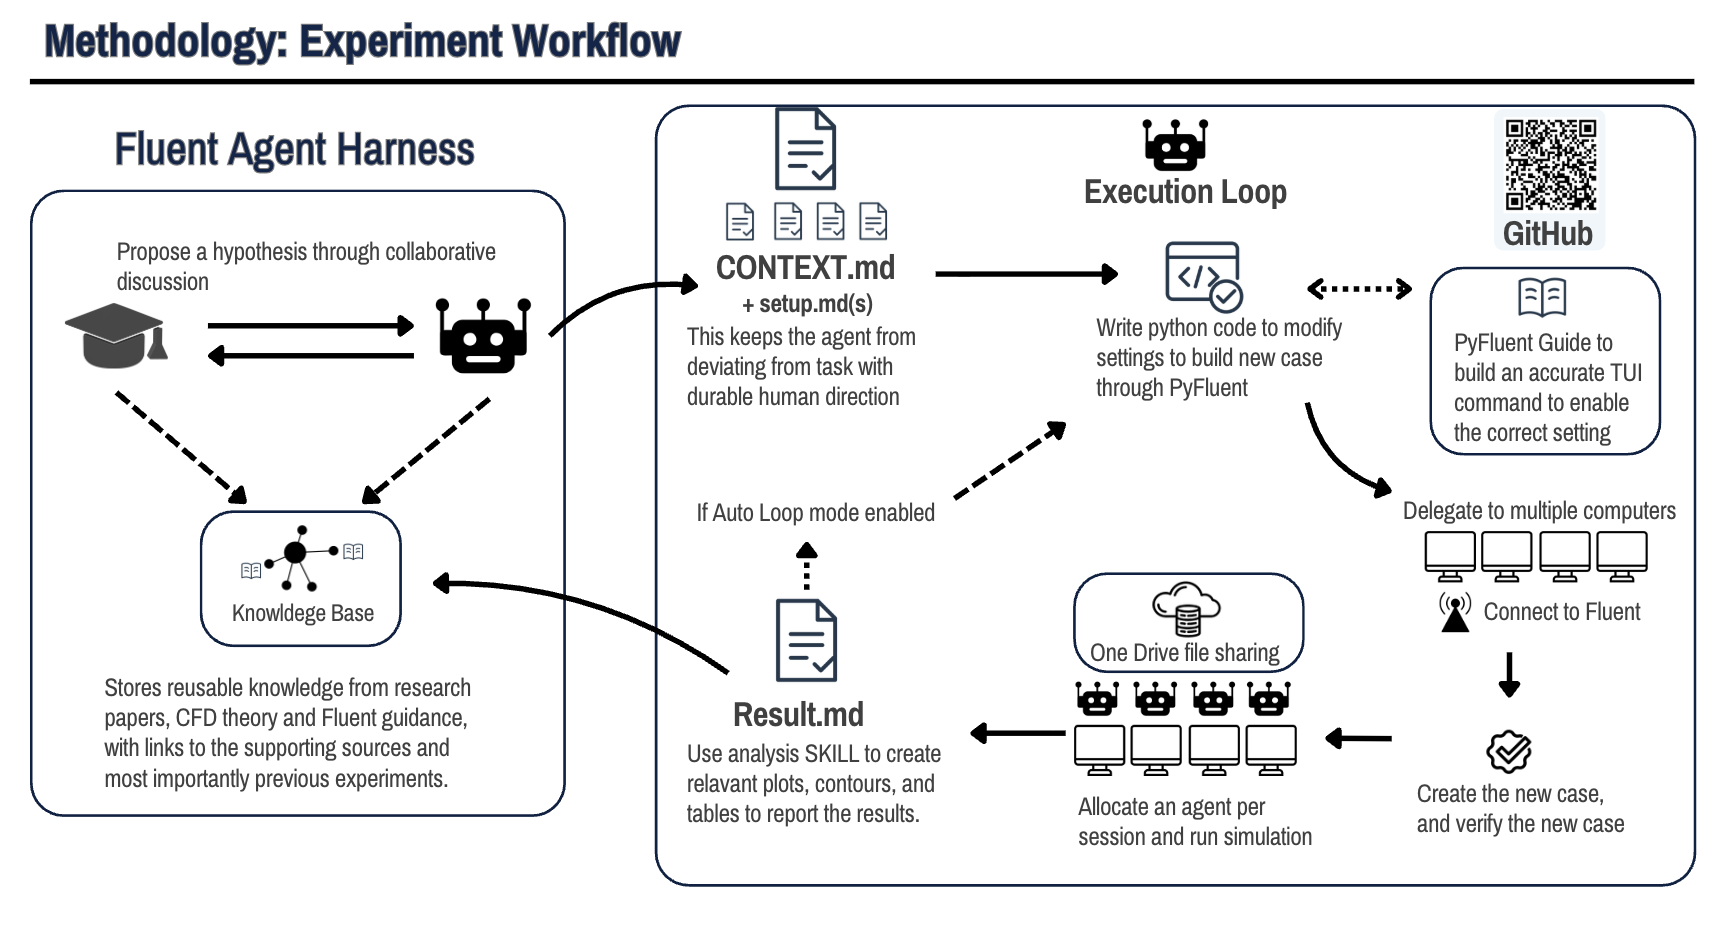
\includegraphics[width=\linewidth]{../../../assets/readme/experiment-workflow.png}

\par\small\textit{Experiment workflow. Source: repository README.}\end{center}

\textbf{Keeping the agent on task.} Durable records gave the agent a defined problem to return to after a long conversation or a failed calculation. \texttt{CONTEXT.md} held the scientific question and permitted scope; \texttt{setup.md} specified the starting case, controlled change, fixed settings and required evidence. Findings and limitations were stored in \texttt{results.md}, while \texttt{phase-state.yaml} recorded the state needed to resume work. These files preserved earlier decisions without relying on conversation memory or repeatedly asking me to reconstruct them.

The directory structure made this information easier to find. \texttt{Project/} held project facts, \texttt{CFD\_wiki/} held reusable literature and methods, \texttt{PyAnsys/} held executable code and machine evidence, and \texttt{.agents/skills/} held procedures. Each fact had one authoritative record, linked from other locations. Focused entry points directed the agent to relevant material. This reduced repeated searches for commands, methods and sources, and helped keep implementation tied to the current question. The structure was intended to limit unsupported assumptions, repeated debugging and irrelevant work, although these problems still occurred.

\textbf{Making progress verifiable.} Custom skills turned broad requests into concrete steps: identify the uncertainty, define a controlled test, inspect the starting case, apply settings in the required order, read back critical values, save and reopen the case, and check a short run before longer execution. Analysis then had to connect the observed fields and histories to the original question. These steps gave the agent observable completion criteria, so a plausible explanation or successful command alone was insufficient.

The custom Model Context Protocol (MCP) integration gave the agent tools to inspect and control Fluent through PyFluent. It extended Ansys's Fluent MCP with controls for attaching to existing sessions, checking generated code and preserving Fluent when the tool connection closed. Reviewed Python/PyFluent scripts handled longer calculations and specialised data extraction. Native solver state, transcripts and paired case/data files provided evidence of what had actually run.

This approach has a parallel in the work of Lauren Tan, a member of technical staff at Cursor, which develops AI coding tools. Her workshop describes the agent-skills framework used within Cursor and released as pstack (\href{https://maven.com/p/e23d9c/how-cursor-turned-ai-agents-into-better-engineers}{Tan, 2026}). Her published verification example gives agents explicit navigation steps and observable evidence checks (\href{https://github.com/poteto/verification-skill-example}{Tan, n.d.}). This provides a practical software-engineering example of making verification part of the agent's task. In CFD, however, verifying execution remains separate from establishing numerical convergence or physical validity.

\textbf{Human judgement and the research opportunity.} Faster execution did not ensure that the next experiment was useful. I was also learning Fluent and CFD, and my limited experience made it harder to recognise which uncertainties mattered. I spent time on investigations that later proved peripheral to the central liquid-routing question. Although the agent could propose and implement tests, I still needed to judge their relevance, interpret unexpected behaviour and decide when to change direction.

I expect that an experienced CFD researcher would use the same harness more effectively by asking sharper questions and recognising unproductive directions earlier. This is my reflection on the project, rather than a measured comparison between users. The experience suggests a promising direction for research: agents can take on more of the repeated implementation, execution and evidence-handling work, allowing researchers to explore more alternatives. Clear human direction and informed interpretation remain essential. The value of faster experimentation depends on the quality of the questions it serves.

% Source: draft/03-results.md

\section{Results}\label{results}

Mesh and inlet comparisons first assess liquid delivery and retention. Collector and startup studies then provide fields for wall comparisons. Finally, film histories test whether captured liquid drains, remains stored or returns to droplets. Earlier exploratory studies are retained in Appendix A.13.

Each comparison uses its stated mesh and settings. Outlet liquid flow is reported as positive outwards unless a signed value is given. Steady-solver iterations track numerical development; accepted film time tracks the transient film calculation.

\subsection{Mesh development and the wall-liquid field}\label{mesh-development-and-the-wall-liquid-field}

Control of spacing near the expected wall-liquid path was the reason for adopting the polyhedral--hexahedral workflow (Figure 7). Wall-following layers provided that control, but topology alone did not establish adequate resolution; Section 3.4 gives the saved near-wall evidence.

The changed wall enrichment at iteration 10,000 shows that the reconstruction produced a different liquid field (Figure 7), but it does not establish greater mesh accuracy. Inlet representation and preparation also changed, and the coarse SIMPLE state had a large mass-balance error. Reduced numerical diffusion remains a possible explanation rather than a measured improvement.

\begin{figure}[!htbp]
\centering
\includegraphics[width=0.98\linewidth,height=0.52\textheight,keepaspectratio]{\detokenize{figures/results-mesh-spatial-comparison.png}}
\caption[Mesh and wall-liquid comparison.]{Mesh and wall-liquid comparison.}
\end{figure}

\subsection{Two-phase inlet and wall-side liquid placement}\label{two-phase-inlet-and-wall-side-liquid-placement}

Inlet phase placement changed the amount of liquid retained under matched conditions (Figure 8). At a nominal speed of 26.81 m/s, the iteration-10,000 inventory increased from 1262.6 kg with mixed feed to 1734.5 kg with split feed: a 37.4\% increase. The same ordering held at all five tested speeds, 20.11--32.14 m/s. Prescribing liquid beside the wall therefore changed the liquid state presented to later wall treatments; it was not a neutral inlet simplification.

Both cases used the same 60,964-cell mesh, phase feed, Coupled settings, initialisation and 10,000-update horizon, with neither collection nor EWF enabled. Figure 8 uses matched inlet-height and centre sections on a shared 0--1 liquid-volume-fraction scale. Complete segregation in the split inlet was an imposed profile (Section 3.3). Over iterations 9500--10,000, steam-outlet liquid flow averaged 99.671\% of the 116.9387 kg/s liquid feed for mixed feed and 99.404\% for split feed. Greater retention therefore did not establish a separate collection route.

\begin{figure}[!htbp]
\centering
\includegraphics[width=0.98\linewidth,height=0.52\textheight,keepaspectratio]{\detokenize{figures/results-inlet-spatial-comparison.png}}
\caption[Liquid distribution with mixed and split feed.]{Liquid distribution with mixed and split feed.}
\end{figure}

\subsection{Liquid accumulation and the need for collection}\label{liquid-accumulation-and-the-need-for-collection}

Low steam-outlet liquid flow was insufficient evidence of collection in the finer absorber-free SIMPLE cases: liquid was being retained without a separate exit (Figure 9). At iteration 3000, the 342,609- and 679,970-cell inventories were about 454--455 kg, while the 997,604-cell case held 333.142 kg and discharged only 0.003623 kg/s. In that finest case, 69.16\% of retained liquid was below \(y=1\) m, identifying the lower vessel as a storage region that needed drainage. These are developing checkpoints, not physical filling histories or a mesh-convergence result; Appendix A.17 retains their exact values.

\begin{figure}[!htbp]
\centering
\includegraphics[width=0.94\linewidth,height=0.43\textheight,keepaspectratio]{\detokenize{../../experiments/phase-08-storyline-reconstruction/stage-02-fine-mesh-simple/direct-student-342k/n3000/figures/matched-mesh-checkpoints.png}}
\caption[Liquid retention without collection.]{Liquid retention without collection.}
\end{figure}

On the 679,970-cell mesh, liquid inventory reached 764.744 kg at iteration 4000, with 69.62\% below \(y=2\) m. Outlet liquid flow was 8.00 kg/s, or 6.84\% of the feed. The next continuation failed after printed iteration 4211; its cause was not isolated.

The inlet and mesh studies changed delivery and retention but provided no separate collection route. The subsequent studies introduced a liquid-selective source after unresolved full-geometry drainage trials (Appendix A.13), then tested startup before comparing wall treatments.

\subsection{Reduced-feed development and inlet ramp}\label{reduced-feed-development-and-inlet-ramp}

The startup and wall studies used the 60,964-cell split-inlet model, with a full feed of 116.92 kg/s liquid and 80.69 kg/s steam.

The late reduced-feed hold provided a comparatively stable inventory for the subsequent loading ramp (Figure 10): mass fell only 0.30\% over iterations 1080--1580, ending at 31.3571 kg. The minimum scaled continuity residual was \(3.2056\times10^{-4}\). These local observations supported using the saved fields as a starting point, without establishing full-feed convergence.

A failed command extended the 25\% hold to iteration 1580. The corrected 2000-update ramp then reached full feed at iteration 3580, with a peak scaled continuity residual of \(1.1166\times10^{-2}\) and peak inventory of 182.5178 kg. The loading disturbance motivated testing activation before the ramp. Figure 10 follows solver iterations, not physical time; its A--C markers distinguish ramp start, full feed with Coupled activation, and later EWF activation.

\begin{figure}[!htbp]
\centering
\includegraphics[width=0.94\linewidth,height=0.43\textheight,keepaspectratio]{\detokenize{figures/results-described-early-development.png}}
\caption[Reduced-feed startup and full-feed development.]{Reduced-feed startup and full-feed development.}
\end{figure}

\subsection{Full-feed control and mass balance}\label{full-feed-control-and-mass-balance}

The smooth-wall, EWF-off Coupled continuation became the iteration-5586 comparison parent. The continuity residual fell and inventory approached 296 kg, but residual oscillations, outlet reverse flow and turbulent-viscosity limiting persisted.

The applied throughput-controlled absorber removal matched its 116.92 kg/s command, but an additional 24.3344 kg/s left through the steam outlet. The signed liquid boundary-plus-source remainder was therefore −24.3344 kg/s, or −20.81\% of the feed. Source application was verified; conservation remained unresolved (Appendix A.15.2).

This developing field supplied a common parent for the following wall comparisons. Changes in outlet flow must be interpreted alongside inventory and removal because the parent did not establish a closed liquid account.

\subsection{Roughness response from the common parent}\label{roughness-response-from-the-common-parent}

Roughness did not provide a consistent means of reducing steam-outlet liquid flow (Figure 11). At \(C_s=0.5\), 0.05 mm roughness raised mean flow by 21.21\%, whereas 8 mm reduced it by 44.09\%, from 24.3715 to 13.6253 kg/s. Increasing \(C_s\) lowered flow at both fixed heights, confirming sensitivity to both inputs. These EWF-off means use iterations 8087--8586 and the smooth-wall reference; they do not identify an optimum surface finish.

\begin{figure}[!htbp]
\centering
\includegraphics[width=0.94\linewidth,height=0.43\textheight,keepaspectratio]{\detokenize{figures/results-described-roughness.png}}
\caption[Roughness sensitivity of outlet liquid flow.]{Roughness sensitivity of outlet liquid flow.}
\end{figure}

The 8 mm case lost 187.109 kg of bulk liquid. Oscillations and incomplete balances prevented an efficiency claim. The later 0.045 mm continuation also changed bulk advancement and film stepping, so it did not isolate the effect of roughness (Appendix A.12).

\subsection{Accretion-enabled wall-film response}\label{accretion-enabled-wall-film-response}

Adding the accretion-enabled EWF package strongly changed steam-outlet liquid flow under common smooth-wall starting fields and throughput collection (Figure 12). Mean flow fell by 92.88\%, from 24.369 to 1.735 kg/s over iterations 8087--8586. The package enabled accretion and coupled film equations at a 10 µs step, with momentum feedback disabled. This comparison establishes sensitivity to the package, rather than the effect of an isolated film term. Earlier trials are documented in Appendix A.11.

\begin{figure}[!htbp]
\centering
\includegraphics[width=0.72\linewidth,height=0.28\textheight,keepaspectratio]{\detokenize{figures/results-described-film-outlet.png}}
\caption[Outlet liquid flow with and without EWF.]{Outlet liquid flow with and without EWF.}
\end{figure}

The lower outlet flow cannot be interpreted as collected liquid. Bulk mass fell from 295.8536 to 63.0234 kg, while film mass reached only 3.1112 kg. The changed wall-adjacent bulk field in Figure 13 is consistent with the new liquid representation, but does not account for that inventory loss. Incomplete combined liquid accounting therefore prevents an efficiency claim. The centre sections at iteration 8586 use the same 0--1 liquid-volume-fraction scale.

\begin{figure}[!htbp]
\centering
\includegraphics[width=0.94\linewidth,height=0.43\textheight,keepaspectratio]{\detokenize{figures/bulk-comparison-described-film-treatment.png}}
\caption[Bulk-liquid distribution with and without EWF.]{Bulk-liquid distribution with and without EWF.}
\end{figure}

The following tests changed the collection and startup settings, then extended film development to examine drainage and storage.

\subsection{Contact collection and combined model development}\label{contact-collection-and-combined-model-development}

A shorter depletion time reduced collector inventory but increased removal variability (Appendix A.4). The combined continuation used contact collection with a 10 µs depletion time, 0.5 mm roughness and a 1 µs film step simultaneously; the effects of these settings were not isolated.

At iteration 45606, film mass was 6.3600 kg after 120.769 ms. Over the final 1000 updates, drainage remained 9.98\% below accretion, so liquid continued to accumulate in the film during this interval. Appendix A.15.3 and the linked case history retain the endpoints and detailed film account.

The shortened-startup comparison below tests whether introducing these treatments before loading reduces the ramp disturbance.

\subsection{Shortened startup with early wall-film activation}\label{shortened-startup-with-early-wall-film-activation}

Activating the combined wall and collection treatment before loading reduced the disturbance during the ramp (Figure 14). Peak continuity residual, bulk + film inventory and outward outlet liquid flow fell by 70.15\%, 70.43\% and 75.78\%, respectively, relative to historical startup. This supports the combined procedure for repeat calculations, but does not isolate which setting produced the reduction. Appendix A.17 lists the peaks. The figure aligns loading progress and excludes the preceding activation hold; negative outlet values indicate outward flow.

\begin{figure}[!htbp]
\centering
\includegraphics[width=0.94\linewidth,height=0.43\textheight,keepaspectratio]{\detokenize{figures/results-described-startup.png}}
\caption[Historical and shortened startup ramps.]{Historical and shortened startup ramps.}
\end{figure}

The excluded activation hold had a continuity residual peak of 0.10593, exceeding the historical ramp peak. At iteration 5080, bulk and film masses were 61.0549 and 0.1645 kg, respectively. Almost all film input was still stored (Appendix A.15.4). All ramp updates met the recorded inner-film tolerance, but 15 of the final 100 hold updates failed to meet it. The startup procedure reduced loading peaks without establishing complete startup convergence (Appendix A.9.4).

The film was still young at full feed. The following continuation held the bulk fields fixed to examine its development under unchanged forcing.

\subsection{Film development under frozen bulk fields}\label{film-development-under-frozen-bulk-fields}

Freezing the bulk fields separated film development from further changes in its forcing (Figures 15--16). After iteration 5080, bulk inventory remained 61.0549 kg and outward bulk-liquid flow remained 3.4300 kg/s by construction. Film mass nevertheless increased from 0.1645 kg at 3.5 ms to 9.5444 kg at 500 ms. This establishes continued surface storage under the retained fields; reciprocal bulk depletion was not calculated.

\begin{figure}[!htbp]
\centering
\includegraphics[width=0.94\linewidth,height=0.43\textheight,keepaspectratio]{\detokenize{figures/results-film-development-reference500ms.png}}
\caption[Film storage and drainage to 500 ms.]{Film storage and drainage to 500 ms.}
\end{figure}

The growing film occupied an increasing part of the wall rather than remaining confined to its early patches (Figure 16). Between 75.66 and 265.18 ms, the wall area at or above 0.10 mm thickness increased from 40.34\% to 61.98\%, while maximum thickness rose from 0.253 to 0.291 mm. Early patchiness was therefore not a stationary distribution under this forcing. The snapshots share a camera and 0--0.30 mm scale.

\begin{figure}[!htbp]
\centering
\includegraphics[width=0.94\linewidth,height=0.43\textheight,keepaspectratio]{\detokenize{figures/wall-film-described-development.png}}
\caption[Wall-film development under frozen bulk forcing.]{Wall-film development under frozen bulk forcing.}
\end{figure}

Developed drainage still did not keep pace with supply (Figure 15). Over the final 10 ms ending at 500 ms, mean accretion was 81.121 kg/s and drainage was 69.600 kg/s, leaving a 14.20\% deficit. The independently calculated mass-change rate was 11.528 kg/s, consistent with continued storage. Substantial drainage therefore did not establish stationary film inventory. Rates use interval-overlap weighting; Appendix A.17 retains the earlier 265.184 ms result and its different 1000-update window. Only the reference-speed arm reached 500 ms (Appendix A.9).

Continued storage motivated tests of two further destinations: release back to droplets and direct removal from the lower wall.

\subsection{Added film-release mechanisms and direct drainage}\label{added-film-release-mechanisms-and-direct-drainage}

A separate configuration enabled stripping, splashing, droplet collection and edge separation while keeping film-to-flow momentum feedback off. Its bulk fields and film forces differed from those of the 500 ms reference. After 4000 bulk updates, 50 ms of frozen-bulk development increased film mass from 0.2638 to 5.9070 kg. Over the final approximately 5 ms, the mean stripping and edge-separation rates were 64.56 and 51.87 kg/s, respectively, while the storage rate was 80.81 kg/s. A separate splash contribution remained unresolved.

The matched direct-drain test established local removal, but the sink throughput overstated the additional external collection (Figure 17). Native film outflow had been zero in the preceding configuration\textquotesingle s final averaging window. After extending EWF onto the lower wall, Drain OFF and ON started from identical fields, a total film mass of 9.7526 kg and the same expanded film domain, with all bulk equations frozen. Over 15 ms, the sink reduced final lower-wall mass by 70.32\%. Its 0.5088 kg removal partly replaced native outflow, so combined external removal increased by only 0.1897 kg. Both removal routes must therefore be counted when judging the benefit.

\begin{figure}[!htbp]
\centering
\includegraphics[width=0.94\linewidth,height=0.43\textheight,keepaspectratio]{\detokenize{figures/results-direct-film-drain.png}}
\caption[Direct drainage: local storage and external removal.]{Direct drainage: local storage and external removal.}
\end{figure}

In the longer continuation, the lower film mass stayed near 0.056 kg while the upper film mass grew. The complete 405 ms record, including the rejected tail, contains 15.16 kg of direct removal and a 27.58 kg increase in film inventory. Film inventory was already increasing before the Courant-guard crossing. Local drainage therefore did not stop accumulation elsewhere. Particle release was internal transfer, while the sink removed liquid from the model (Appendix A.12).

The following numerical checks assess source application and film-step selection. The final mesh comparison addresses resolution separately.

\subsection{Numerical assessment of the selected development path}\label{numerical-assessment-of-the-selected-development-path}

The shortened-startup contact source matched independently evaluated removal at all 3500 solved updates. A separate film-step test starting from identical fields showed that a 20 µs film step passed local field and ledger checks over 2.5 ms, whereas a 25 µs film step exceeded the 0.1\% ledger-error limit.

These checks supported implementation and local step selection. Inner-film failures and unavailable residuals prevented a numerical convergence claim, while continued storage prevented a stationary-film claim (Appendix A.9.4).

\subsection{Mesh sensitivity of film development and drainage}\label{mesh-sensitivity-of-film-development-and-drainage}

After introducing film formation, release and lower-wall removal, the next question was whether the predicted liquid paths persisted across mesh resolutions. The observation time was chosen from the coarse-mesh drainage behaviour described in Section 3.6. Comparing the selected states at 195 ms tested what each calculation predicted at the same film age, before any claim of equilibrium collection.

\begin{figure}[!htbp]
\centering
\includegraphics[width=0.98\linewidth,height=0.52\textheight,keepaspectratio]{\detokenize{../../experiments/phase-09-mesh-convergence/figures/selected-film-thickness.png}}
\caption[Wall-film distribution across meshes at 195 ms.]{Wall-film distribution across meshes at 195 ms.}
\end{figure}

The common film age did not produce a common spatial state (Figure 18). Similarity between the 342k and 680k patterns was insufficient to establish convergence because the 997k state differed again. This limits the use of a coarse-mesh drainage timescale for judging finer-mesh development. The maps share a clipped 0--0.30 mm thickness scale and exclude the lower collector and inlet extension; arrows indicate direction only. A snapshot comparison cannot determine propagation speed.

\begin{figure}[!htbp]
\centering
\includegraphics[width=0.94\linewidth,height=0.43\textheight,keepaspectratio]{\detokenize{../../experiments/phase-09-mesh-convergence/figures/selected-mesh-response.png}}
\caption[Liquid inventories and removal across meshes.]{Liquid inventories and removal across meshes.}
\end{figure}

Agreement between the intermediate meshes did not persist on the finest completed mesh (Figure 19). Film inventories at 195 ms were 7.490, 2.821, 2.950 and 2.056 kg on the 60k, 342k, 680k and 997k meshes. Although the intermediate inventories differed by only 4.6\%, the 997k inventory was 30.3\% lower than 680k and its drain rate was 32.3\% lower. These are saved endpoints under frozen bulk forcing, not history means. The 342k starting reference precedes an additional bulk-active adjustment; the 2.6M reference has provisional settings and no 195 ms endpoint.

The lower drain rates reflect less liquid available to the same sink law, rather than a separate loss of sink effectiveness. Lower-wall inventories of 34.07, 10.75, 10.17 and 6.88 g gave endpoint rates of 22.716, 7.168, 6.778 and 4.587 kg/s when divided by the prescribed 1.5 ms capture time. These rates are not cumulative collection. The bulk outlet values in Figure 19 exclude internal sources, so they cannot complete a liquid balance.

The common observation time did not produce equivalent film distributions. The maps are consistent with slower film propagation on the finer meshes, but lower supply or greater release could also reduce the visible coverage and inventory. Section 5.1 discusses these alternatives. Continuous selected-run inventory, flux and film-source histories were unavailable in the shared evidence, and saved bulk residuals were partly decimated. Unchanged bulk quantities during the frozen stage follow from the procedure and do not demonstrate convergence. These endpoints establish neither mesh independence nor stationary film storage, a complete liquid balance or total separator efficiency.

% Source: draft/04-discussion-conclusions-and-future-work.md

\section{Discussion}\label{discussion}

The results identify three linked model sensitivities: liquid delivery to the wall, transfer into the wall film and removal from the vessel. These responses must be considered together to assess collection; the explanations for some changes remain unresolved.

\subsection{Mesh development changed the wall-liquid representation}\label{mesh-development-changed-the-wall-liquid-representation}

The polyhedral--hexahedral workflow made wall refinement and coarse local testing more practical. This matters because the liquid path of interest occupies the wall region, where fine cross-wall spacing is needed to represent steep liquid-fraction gradients. The wall layers provided control over that spacing, while larger interior cells supported less costly exploratory calculations. A reduction in numerical smearing remains a hypothesis because transport error also depends on resolution, alignment and discretisation (\href{https://ansyshelp.ansys.com/public/Views/Secured/corp/v252/en/flu_ug/flu_ug_GridTypes.html}{Ansys, Inc., 2025c, §7.1.3.3}).

The broader liquid-rich region in Figure 7 suggested that wall liquid was being represented differently. The finer absorber-free calculations then showed much of the retained liquid near the wall and base, with little passing through the steam outlet (Figure 9). These observations support the concern that a model that retains liquid away from steam also needs a collection route. The later failure of these calculations did not establish greater mesh accuracy or identify the cause of numerical breakdown.

Historical comparisons cannot isolate mesh effects because inlet representation and preparation also changed and matched inventory histories were unavailable. The combined-model comparison adds a common-film-age assessment of distribution, storage and drainage (Section 4.13). Its main implication is that the observation time chosen from coarse-mesh drainage did not produce equivalent film distributions across resolutions. The finer cases showed less extensive appreciable film thickness and lower drainage at 195 ms (Figures 18--19), consistent with delayed film propagation towards collection. A coarse-mesh drainage response that begins to level out is therefore insufficient to establish that the finer cases have reached the same stage of development.

Transport delay alone does not explain the lower total film inventory. If supply and release were otherwise equal, reduced drainage would leave more liquid stored on the wall. The combination of lower storage and lower drainage therefore requires consideration of differences in film supply, release and their histories as well as transport. The drain law itself remained proportional to local lower-wall inventory: the lower endpoint rate reflected less liquid in that region under the same removal timescale. Missing source histories prevent these contributions from being separated.

The broad coarse-mesh coverage may partly reflect numerical spreading, whereas finer resolution may preserve more distinct liquid paths. This remains a hypothesis: the retained bulk fields and preparation also differed, affecting the conditions that supply and drive the film. The two intermediate meshes showed similar patterns, but the 997k result did not establish a common limiting state. Equal-age comparisons remain useful for transient predictions; longer histories are needed to determine whether the differences represent a delay, distinct later drainage levels, or both.

\subsection{Inlet phase placement changes the wall-liquid starting condition}\label{inlet-phase-placement-changes-the-wall-liquid-starting-condition}

The thin liquid strip provided a reproducible way to prescribe the wall-rich feed. Liquid films in upstream piping provide a physical reason to test that placement but do not establish the actual inlet profile (\href{https://publications.mygeoenergynow.org/grc/1028587.pdf}{Pointon et al., 2009}).

The matched inlet comparison shows why inlet placement must be held fixed when assessing wall treatment (Figure 8). Wall-side placement increased retained liquid by 37.4\%, changing the liquid distribution supplied to the wall before EWF was added. Almost all feed still left through the steam outlet, so this sensitivity concerns the starting condition for collection rather than improved separation. Later comparisons must follow storage and removal under the same inlet assumption.

\subsection{The central development problem was the liquid collection route}\label{the-central-development-problem-was-the-liquid-collection-route}

The closed-bottom model's only exit was the steam outlet. Liquid in the model either accumulated or left with steam, whereas separator operation requires outward transport followed by brine discharge. The rising liquid inventory was consistent with the missing drain, but changes over steady-solver iterations did not provide a physical filling rate (\href{https://doi.org/10.1016/j.geothermics.2014.05.009}{Zarrouk \& Purnanto, 2015}).

The absorber-free Coupled cases discharged 99.4--99.7\% of the liquid feed through the steam outlet. Their smaller mass imbalance did not make this liquid exit route suitable for collection. In a stationary closed-bottom calculation without another sink, conservation would require incoming liquid to leave through that outlet. Numerical closure can therefore be desirable while the available boundary routes remain inadequate for the separator question. This distinction explains why Coupled remained useful after a collector was added.

Opening the lower boundary allowed steam to leave through it. Full-geometry trials exposed dependence on a liquid seal and outlet control; neither an initially patched pool nor the tested pressure feedback established a maintained pool. Explicit liquid collection in the truncated vessel allowed wall studies to continue. This collection approach represents transfer to an omitted pool without predicting its pressure, level or discharge response.

\subsection{Contact removal and staged startup made the model easier to develop}\label{contact-removal-and-staged-startup-made-the-model-easier-to-develop}

The contact absorber tied removal of mass and momentum to liquid present in the collector. This dependence on local liquid presence more closely reflected the intended transfer to the omitted pool than removal prescribed from inlet throughput alone.

Reduced feed allowed flow and collection to develop before full loading. This useful hold arose after a ramp command failed; the checked ramp converted the observation into a repeatable startup procedure. With the later contact and film treatments activated before loading, ramp peaks in the continuity residual, combined bulk + film inventory and outlet flow were about 70\%, 70\% and 76\% lower, respectively.

The shorter procedure supported repeat runs on finer meshes but changed several settings together. The larger activation disturbance occurred before the ramp comparison, so the smaller ramp peaks do not describe the whole startup. The causes of that disturbance and later film-solver failures remain unresolved. Comparable starts require checked fields and film ages.

\subsection{Wall treatment strongly controls the calculated liquid state}\label{wall-treatment-strongly-controls-the-calculated-liquid-state}

The non-monotonic roughness response in Figure 11 shows that increasing the roughness input did not consistently reduce outlet liquid flow. Small roughness heights raised outlet liquid flow, while the largest tested height reduced it by 44.09\%. Roughness changes the modelled near-wall momentum transfer; it does not supply a new liquid store or drain. (\href{https://ansyshelp.ansys.com/public/Views/Secured/corp/v252/en/flu_th/x1-5720008.164.html}{Ansys, Inc., 2025k}) One possible explanation for the outlet response is a change in liquid transport or residence near the wall. A competing explanation is reduced liquid availability after bulk inventory depletion. The 8 mm case lost 187.109 kg during the continuation, so depletion remains a possible explanation even though the final outlet history became comparatively level. The wall-surface velocity report sampled the no-slip boundary and could not resolve the near-wall transport needed to distinguish these explanations.

The accretion-enabled film package added surface storage and transport, but its lower bulk outlet flow did not resolve the liquid account (Figures 12--13). The small final film inventory did not explain the large loss of bulk mass. Neither an outlet reduction nor a visible change beside the wall can therefore establish where the liquid went. A complete bulk, source and film account is needed before assigning a collection benefit.

These screens identify wall treatment as a major model sensitivity. The 8 mm screen and later 0.045 mm material-reference continuation also used different bulk advancement and film stepping. Neither identified an optimum surface finish. A useful follow-up must distinguish increased delivery to the collector from bulk-liquid depletion, surface storage and transfer back to droplets. Such a comparison requires wall-adjacent fields and separate inventories and removal histories, alongside comparable bulk advancement and film stepping, rather than an outlet ranking alone.

\subsection{Film development, release and drainage answer different parts of the same question}\label{film-development-release-and-drainage-answer-different-parts-of-the-same-question}

The film histories show why an early wall snapshot is insufficient to assess collection (Figures 15--16). Continued spreading changed the available surface storage, and substantial late drainage still coexisted with positive accumulation. The remaining 11.53 kg/s storage rate at 500 ms means that drainage had not balanced supply. Longer development therefore changed the interpretation from initial capture to an unresolved balance between delivery, transport and removal.

The bulk fields were frozen during this development, so the film responded to fixed forcing. This choice held the bulk inventory and outlet flux constant; the bulk was not updated to account for depletion. The run reveals how the film develops under those fields, while sustained coupled collection remains a separate question.

In later runs with different fields and film forces, stripping and edge-separation records showed film liquid returning as droplets. Splashing was enabled but not measured separately. Release from the film reduces film mass without necessarily removing liquid from the vessel: the droplets may return to the wall, enter the collector or leave with steam. This modelled release is consistent with the film-entrainment problem described in the literature and explains why wall capture alone cannot establish permanent collection (\href{https://www.researchgate.net/publication/310818568_LIQUID_CARRYOVER_IN_GEOTHERMAL_STEAM-WATER_SEPARATORS}{Rizaldy et al., 2016}; \href{https://ansyshelp.ansys.com/public/Views/Secured/corp/v252/en/flu_th/flu_th_ewf_sec_film_submodels.html}{Ansys, Inc., 2025b}).

The matched direct-drain test demonstrated local film removal with the bulk equations frozen (Figure 17). Lower-wall inventory fell by 70.32\%, but the 0.5088 kg removed by the direct sink partly replaced native film outflow, which fell from 0.5302 to 0.2111 kg. Combined removal increased by only 0.1897 kg, close to the reduction in total film inventory. The sink therefore changed the distribution of removal between routes while also increasing total removal. The mass removed by the direct sink alone would overstate the gain relative to the drain-OFF arm.

In the longer continuation, film inventory in the lower region stayed near 0.056 kg while almost all film growth occurred above it. Removal was active, yet input still exceeded the combined losses; film continued to accumulate in the upper region before the later Courant-guard failure. These observations raise questions about film transport towards the collector as well as local drainage. They do not establish that downward motion was absent or isolate the cause of upper accumulation. Features that intercept circulating film or guide it towards the collector are specific design hypotheses. Assessing these features requires tracking collection, steam-outlet liquid, storage and pressure loss together, because lower film mass could also result from greater release into the steam flow.

\subsection{Contribution and the evidence needed for performance prediction}\label{contribution-and-the-evidence-needed-for-performance-prediction}

The contribution is a model-development approach that follows liquid from its assumed inlet placement through wall transport to collection. Checked collection and startup procedures enabled the comparisons; longer histories distinguished storage, release and drainage. Appendix B summarises the supported answers in Table B2.

Bulk-liquid flux, outlet quality and DPM escape fractions measure different quantities. Exact absorber tracking did not close the early balance, and a small film-ledger error did not establish whole-separator conservation. Assessing whole-separator conservation requires each liquid transfer to be tracked and counted once.

High wall \(y^+\) values in the saved fields, incomplete refinement assessment and omitted pool response limit performance prediction. Physical validation still requires comparison with measurements under matched operating conditions and at corresponding locations, together with an assessment of uncertainty (\href{https://www.grc.nasa.gov/www/wind/valid/tutorial/valassess.html}{NASA, 2021b}).

The common-age mesh comparison also shows why the collection model must be assessed through its developing liquid paths. A drainage level on one mesh cannot be assumed to represent the same film-development stage on another. The present evidence does not select a mesh for quantitative performance prediction.


\section{Conclusions and future work}\label{conclusions-and-future-work}

\subsection{Conclusions}\label{conclusions}

Liquid reaching the wall did not by itself establish collection. This study developed a geothermal separator CFD model by tracking where liquid enters, accumulates, transfers and leaves. Mesh and inlet investigations showed that the predicted wall-liquid distribution depended on how wall liquid was represented. In the matched inlet comparison, placing liquid beside the wall increased retained mass by 37.4\%. Absorber-free cases showed the consequences of a missing collection route: liquid accumulated or was discharged almost completely through the steam outlet.

A liquid-selective absorber and staged loading supplied common fields for wall studies. The contact treatment represented the transfer of liquid mass and momentum to the omitted brine pool. The later combined startup reduced the peak continuity residual during the ramp by 70.15\%, but a separate activation disturbance remained.

Wall treatment changed both bulk-liquid discharge and liquid storage in the model. The selected accretion-enabled film package reduced mean bulk-liquid outlet flow from 24.369 to 1.735 kg/s, alongside a large decrease in bulk-liquid inventory. With the bulk fields held fixed, the film calculations predicted spreading, thickening and drainage, but the film storage rate still averaged 11.53 kg/s over the final 10 ms ending at 500 ms. The direct drain removed 0.5088 kg but increased combined external removal by only 0.1897 kg because it partly replaced native film outflow. The mass removed by the direct drain alone therefore overstated the additional collection. These calculations showed that lower-wall collection could operate while film continued to accumulate above it.

The completed work demonstrates model sensitivity and provides checked procedures for collection and startup. These findings motivate tests of designs that redirect wall liquid towards collection. At 195 ms, finer-mesh states showed less extensive appreciable film thickness and lower film drainage. The coarse-informed observation time did not establish equivalent film development across resolutions. This is consistent with slower propagation, but differences in film supply and release remain unresolved; mesh independence has not been established. Sustained liquid accounting and physical validation are still needed before claiming improved separation efficiency or pressure-drop accuracy.

\subsection{Future work}\label{future-work}

The next comparisons should test the proposed explanations and address the remaining evidence gaps:

\begin{enumerate}
\def\labelenumi{\arabic{enumi}.}
\tightlist
\item
  \textbf{Resolve the mesh dependence of film development.} Compare film coverage, supply, storage, release and drainage histories using controlled preparation and checked film steps. Retain equal-age comparisons and extend development to distinguish delayed propagation from different later drainage levels. Test whether the broad coarse-mesh coverage reflects numerical spreading or differences in film supply and forcing.
\item
  \textbf{Complete the coupled liquid account.} Advance the bulk equations and track bulk, film and droplet transfers together. Separate external removal from internal transfers and repeat developed-film step checks.
\item
  \textbf{Separate startup and model effects.} Compare loading sequence, collector law and solver controls individually from common fields.
\item
  \textbf{Compare with measurements.} Match feed conditions and the locations of pressure and liquid measurements to assess the model's use for design.
\end{enumerate}

\subsubsection{Proposed inlet-region designs}\label{proposed-inlet-region-designs}

The wall-film studies suggest that a design should control what happens after liquid reaches the wall. Film continued to accumulate above the lower collector, and the release models provided routes for liquid to return to the steam. These findings motivate two related questions: can a feature intercept circulating wall liquid before it meets the incoming steam again, and can it guide that liquid towards collection? The design proposals developed for the project poster address these questions, but their effect on separation performance remains unverified.

The \textbf{vertical film blocker} is intended to interrupt circumferential liquid transport and reduce renewed contact with incoming steam. The \textbf{angled film ramp} is intended to guide liquid towards the lower collector. Figure 20 places these hypotheses in their local bulk-flow context, but mixture-velocity vectors cannot establish that wall film follows either intended route. The manual views are associated with the basic-EWF 50 ms case folders: 154,063 cells for the blocker and 213,232 for the ramp. Their cameras, vector sampling and lower colour limits differ, although both upper limits are 60 m/s; they do not support a quantitative velocity comparison.

\begin{figure}[!htbp]
\centering
\begin{minipage}[t]{0.49\linewidth}\centering
\includegraphics[height=0.17\textheight,keepaspectratio]{\detokenize{../../experiments/phase-10-proposed-design/figures/manual-vertical-blocker-basic-50ms.png}}
\par\small (a) Vertical film blocker
\end{minipage}
\begin{minipage}[t]{0.49\linewidth}\centering
\includegraphics[height=0.17\textheight,keepaspectratio]{\detokenize{../../experiments/phase-10-proposed-design/figures/manual-angled-ramp-50ms.png}}
\par\small (b) Angled film ramp
\end{minipage}
\caption[Proposed film blocker and ramp.]{Proposed film blocker and ramp.}
\end{figure}

Both basic-wall-film calculations subsequently reached a film age of 150 ms. Over 50--150 ms, they used matching basic film settings and fixed 10 µs steps with the bulk fields held fixed (Appendix A.14). This established retained states for further assessment, but the meshes, initial bulk fields and earlier film histories differed. Moreover, stripping and edge separation were disabled in these basic-film continuations. They therefore cannot test whether either feature suppresses renewed droplet release. The earlier near-50 ms inlet comparison used a separate enhanced-film vertical case; its local film values must not be treated as results from the matching basic-film comparison.

A third concept is an \textbf{external collection channel}: a shell opening would intercept wall liquid and lead it into an external drain. This would provide a route out of the main swirling region. It remains a proposal without selected simulation evidence. Its assessment would need to include the pressure and liquid-seal conditions that permit liquid discharge while limiting steam loss, because the earlier full-geometry trials showed that an open lower route could also discharge steam.

A useful design comparison should include the unmodified geometry and both internal features under controlled feed, model settings and preparation. Local mesh refinement and film-step checks are needed around each feature, followed by histories long enough to distinguish transport delay from a sustained change in collection. The comparison should track collected liquid, liquid leaving with steam, film storage and release, and inlet-to-outlet pressure loss. Bulk, film and droplet transfers must be accounted for together. Lower film inventory would support the intended design only if liquid reached collection rather than returning to the steam. This would test whether intercepting or redirecting wall liquid improves the complete collection route identified by this study.

\clearpage\ESBfrontsection{Acknowledgements}
I thank Sadiq Zarrouk and Maedeh Amirpour for their supervision and feedback as the modelling questions developed. Discussions with Sadiq also helped shape the wall-liquid design concepts. I thank Andy Tran for his collaboration as my project partner.

\clearpage\ESBfrontsection{References}\begingroup\raggedright\interlinepenalty=10000\setlength{\parindent}{-1.27cm}\setlength{\leftskip}{1.27cm}
Ansys, Inc.~(2025a). Cell zone conditions (§8.2.7, Defining mass, momentum, energy, and other sources). In \emph{Ansys Fluent user's guide} (Release 2025 R2). \url{https://ansyshelp.ansys.com/public/Views/Secured/corp/v252/en/flu_ug/flu_ug_bcs_sec_cell_zones.html\#flu_ug_sec_bc_source}



Ansys, Inc.~(2025b). Film sub-models (§17.2.1). In \emph{Ansys Fluent theory guide} (Release 2025 R2). \url{https://ansyshelp.ansys.com/public/Views/Secured/corp/v252/en/flu_th/flu_th_ewf_sec_film_submodels.html}



Ansys, Inc.~(2025c). Mesh topologies (§7.1, particularly §7.1.3.3, Numerical diffusion). In \emph{Ansys Fluent user's guide} (Release 2025 R2). \url{https://ansyshelp.ansys.com/public/Views/Secured/corp/v252/en/flu_ug/flu_ug_GridTypes.html}



Ansys, Inc.~(2025d). Mixture model theory (§14.4, particularly the overview and relative-velocity formulation). In \emph{Ansys Fluent theory guide} (Release 2025 R2). \url{https://ansyshelp.ansys.com/public/Views/Secured/corp/v252/en/flu_th/flu_th_sec_multiphase_mixture.html}



Ansys, Inc.~(2025e). Modeling Eulerian wall films (Chapter 30, particularly §§30.3--4). In \emph{Ansys Fluent user's guide} (Release 2025 R2). \url{https://ansyshelp.ansys.com/public/views/secured/corp/v252/en/flu_ug/flu_ug_models_wallfilm.html}



Ansys, Inc.~(2025f). Model-specific DEFINE macros (§2.3.45, DEFINE\_SOURCE). In \emph{Ansys Fluent customization manual} (Release 2025 R2). \url{https://ansyshelp.ansys.com/public/Views/Secured/corp/v252/en/flu_udf/flu_udf_ModelSpecificDEFINE.html\#flu_udf_sec_define_source}



Ansys, Inc.~(2025g). Numerical schemes and solution algorithm (§17.4). In \emph{Ansys Fluent theory guide} (Release 2025 R2). \url{https://ansyshelp.ansys.com/public/Views/Secured/corp/v252/en/flu_th/flu_th_ewf_sec_num_schemes.html}



Ansys, Inc.~(2025h). Overview of using the Eulerian wall film model (§30.2). In \emph{Ansys Fluent user's guide} (Release 2025 R2). \url{https://ansyshelp.ansys.com/public/views/secured/corp/v252/en/flu_ug/flu_ug_ewf_sec_overview.html}



Ansys, Inc.~(2025i). Pressure-based solver settings (§37.3, particularly §37.3.1, Choosing the pressure--velocity coupling method). In \emph{Ansys Fluent user's guide} (Release 2025 R2). \url{https://ansyshelp.ansys.com/public/Views/Secured/corp/v252/en/flu_ug/flu_ug_sec_uns_solve_pvel_1.html}



Ansys, Inc.~(2025j). Solution strategies for multiphase modeling (§27.8, particularly §§27.8.1.2--1.3 and 27.8.1.7). In \emph{Ansys Fluent user's guide} (Release 2025 R2). \url{https://ansyshelp.ansys.com/public/Views/Secured/corp/v252/en/flu_ug/flu_ug_sec_multiphase_solution.html}



Ansys, Inc.~(2025k). Wall roughness effects in turbulent wall-bounded flows (§4.18.5). In \emph{Ansys Fluent theory guide} (Release 2025 R2). \url{https://ansyshelp.ansys.com/public/Views/Secured/corp/v252/en/flu_th/x1-5720008.164.html}



International Association for the Properties of Water and Steam. (2012). \emph{Revised release on the IAPWS industrial formulation 1997 for the thermodynamic properties of water and steam} (R7-97{[}2012{]}). \url{https://iapws.org/technical-guidance/release/IF97-Rev}



National Aeronautics and Space Administration. (2021a, February 10). \emph{Examining iterative convergence}. NPARC Alliance CFD verification and validation tutorial. \url{https://www.grc.nasa.gov/www/wind/valid/tutorial/iterconv.html}



National Aeronautics and Space Administration. (2021b, February 10). \emph{Validation assessment}. NPARC Alliance CFD verification and validation tutorial. \url{https://www.grc.nasa.gov/www/wind/valid/tutorial/valassess.html}



National Aeronautics and Space Administration. (2021c, February 10). \emph{Verification assessment}. NPARC Alliance CFD verification and validation tutorial. \url{https://www.grc.nasa.gov/www/wind/valid/tutorial/verassess.html}



Pointon, A. R., Mills, T. D., Seil, G. J., \& Zhang, Q. (2009). Computational fluid dynamic techniques for validating geothermal separator sizing. \emph{GRC Transactions, 33}, 943--948. \url{https://publications.mygeoenergynow.org/grc/1028587.pdf}



Purnanto, M. H., Zarrouk, S. J., \& Cater, J. E. (2013). CFD modelling of two-phase flow inside geothermal steam--water separators. \emph{IPENZ Transactions, 40}, 1--10. \url{https://www.researchgate.net/publication/269519626_CFD_MODELLING_OF_TWO-PHASE_FLOW_INSIDE_GEOTHERMAL_STEAM-WATER_SEPARATORS}



Rizaldy, Zarrouk, S. J., \& Morris, C. (2016). Liquid carryover in geothermal steam--water separators. In \emph{Proceedings of the 38th New Zealand Geothermal Workshop}, Auckland, New Zealand. \url{https://www.researchgate.net/publication/310818568_LIQUID_CARRYOVER_IN_GEOTHERMAL_STEAM-WATER_SEPARATORS}



Skoog, E. (2020). \emph{CFD annular flow modelling based on a three-field approach} {[}Master's thesis, Luleå University of Technology{]}. DiVA. \url{https://www.diva-portal.org/smash/get/diva2:1452100/FULLTEXT02.pdf}



Tan, L. [poteto]. (n.d.). \emph{Verification-skill-example: Project-local verification skill and feature map} [Example repository]. GitHub. Retrieved October 17, 2026, from \url{https://github.com/poteto/verification-skill-example}.

Tan, L. (2026, August 12). \emph{How Cursor turned AI agents into better engineers} [Workshop]. Maven. \url{https://maven.com/p/e23d9c/how-cursor-turned-ai-agents-into-better-engineers}.

Zarrouk, S. J., \& Purnanto, M. H. (2015). Geothermal steam--water separators: Design overview. \emph{Geothermics, 53}, 236--254. \url{https://doi.org/10.1016/j.geothermics.2014.05.009}


The design overview is cited as 2015, following the volume-publication metadata. Its local filename, PDF header and wiki label use 2014.

\endgroup
\clearpage\ESBappendix
\renewcommand{\thefigure}{\thesection\arabic{figure}}\renewcommand{\thetable}{\thesection\arabic{table}}
\clearpage

\section{Method detail and reproducibility}\label{appendix-a.-method-detail-and-reproducibility}

\subsection{Verified model inputs and remaining evidence}\label{a.1.-verified-model-inputs-and-remaining-evidence}

\begingroup\small\setlength{\tabcolsep}{3pt}
\begin{longtable}[]{@{}
  >{\raggedright\arraybackslash}p{(\linewidth - 4\tabcolsep) * \real{0.3333}}
  >{\raggedright\arraybackslash}p{(\linewidth - 4\tabcolsep) * \real{0.3333}}
  >{\raggedright\arraybackslash}p{(\linewidth - 4\tabcolsep) * \real{0.3333}}@{}}
\caption{Model inputs and source records for the selected startup and absorber studies. Unverified settings remain case-specific gaps.}\tabularnewline
\toprule\noalign{}
\begin{minipage}[b]{\linewidth}\raggedright
Setting group
\end{minipage} & \begin{minipage}[b]{\linewidth}\raggedright
Verified basis
\end{minipage} & \begin{minipage}[b]{\linewidth}\raggedright
Evidence and remaining limits
\end{minipage} \\
\midrule\noalign{}
\endfirsthead
\toprule\noalign{}
\begin{minipage}[b]{\linewidth}\raggedright
Setting group
\end{minipage} & \begin{minipage}[b]{\linewidth}\raggedright
Verified basis
\end{minipage} & \begin{minipage}[b]{\linewidth}\raggedright
Evidence and remaining limits
\end{minipage} \\
\midrule\noalign{}
\endhead
\bottomrule\noalign{}
\endlastfoot
Bulk formulation & Pressure-based solver, absolute velocity; Mixture; RNG \(k\)--\(\varepsilon\) with differential-viscosity and swirl options and standard wall functions; gravity \((0,-9.81,0)\) m/s²; energy off & \href{draft/../../../experiments/phase-07-1a-absorber-convergence/baseline-v2-virtual-liquid-outlet/build-manifest.json}{Throughput-collector build and readback}; selected model described in Section 3.2 \\
Geometry and mesh & 60,964 cells, 226,982 nodes and 328,287 faces; identical geometry and connectivity in the full-feed parent, combined contact endpoint and shortened-startup endpoint; 715 collector cells selected by centroid \(y\leq0.10\) m & Figure 6 and Appendix A.10 give boundaries, dimensions and source-region extent. The earlier 342,609-cell collector and later meshes are separate cases \\
Wall resolution and quality & Native shared-flow \texttt{SV\_WALL\_YPLUS}, \texttt{SV\_WALL\_YPLUS\_UTAU} and adjacent-cell \texttt{SV\_WALL\_DIST} recovered from three hash-matched data pairs & Appendix A.10 gives per-wall area-weighted statistics. Exact meshing layer count/first-layer height and solver-side orthogonal quality/skewness remain unverified; no completed matched refinement study \\
Feed & Enthalpy and phase-flow calculation in Section 3.3.1 and Appendix A.7; hold: 29.23/20.1725 kg/s liquid/vapour; full feed: 116.92/80.69 kg/s & Boundary readbacks and the discrete ramp rule are in the \href{draft/../../../experiments/phase-07-1a-absorber-convergence/roughness-family/r0-smooth-control/provenance.md}{startup provenance} \\
Materials and walls & Density and viscosity for the throughput-controlled absorber model in Section 3.2; smooth-wall parent & Full-precision values are in the \href{draft/../../../experiments/phase-07-1a-absorber-convergence/baseline-v2-virtual-liquid-outlet/build-manifest.json}{material settings}; wall treatments are recorded for each selected case \\
Phase interaction & Manninen algebraic slip; Schiller--Naumann drag; constant phase-2 diameter \(10^{-5}\) m (10 µm). Virtual mass, lift, wall lubrication, turbulent dispersion and turbulence interaction off; bulk surface tension/cavitation off; no bulk interphase mass-transfer model & Recovered from the hash-matched full-feed parent/control at iteration 5586, combined contact endpoint at iteration 45606 and shortened-startup endpoint at iteration 5080. See \href{draft/../figures/model-domain-metadata.json}{saved-case model and geometry metadata}. EWF phase accretion is a separate wall transfer \\
Boundary settings & Pure-phase mass-flow inlets and steam pressure outlet in the main lineage; full-feed-control settings in Appendix A.6 & Pressure, turbulence, hydraulic-diameter and backflow values apply to the identified saved control; they are not assumed for other branches \\
Historical startup & Actual 25\% hold to iteration 1580; 2000-update ramp to iteration 3580; Coupled/Global Time Step continuation to iteration 5586 & The \href{draft/../../../experiments/phase-07-2a-wall-liquid-routing/stage-02-combined-ewf-roughness/case-history-N45606.md}{selected native history} distinguishes the intended schedule from the executed sequence \\
Full-feed control & Terminal control separated from hold, ramp and warm-up; settings in Appendix A.6 & Full readbacks are in the \href{draft/../../../experiments/phase-07-1a-absorber-convergence/roughness-family/r0-smooth-control/setup.md}{control setup}; the \href{draft/../../../experiments/phase-07-1a-absorber-convergence/roughness-family/r0-smooth-control/control-window.md}{declared window} defines the comparison \\
Final contact absorber & \(S_L=-\rho_L\alpha_L/\tau\); \(\tau=10^{-5}\) s; liquid-velocity momentum removal; \texttt{libcontactv2} & Derivative and hook identities are given in Appendix A.3, with the \href{draft/../../../experiments/phase-07-2a-wall-liquid-routing/stage-02-combined-ewf-roughness/ewf-absorber/setup.md}{contact-treatment setup} \\
Roughness screen & Common full-feed-parent fields at iteration 5586; EWF off; 3000 updates; final-500 means & Heights, constants, inventory changes and oscillations are in the \href{draft/../../../experiments/phase-07-2a-wall-liquid-routing/roughness-family/results.md}{roughness-screen results} \\
Film-disabled/accretion-enabled comparison & Smooth walls; EWF off/on package; accretion on in the film case; film equations coupled; wall momentum feedback off; fixed 10 µs film step & Exact mechanisms and numerical readbacks in Appendix A.9; \href{draft/../../../../PyAnsys/output/phase72a_ewf_student_e27_build_20260923T071523Z/probe-receipt.json}{accretion-enabled film build/reopen receipt} \\
Combined lineage & Original accretion-enabled film fields; later roughness, contact absorber and smaller film step; selected replay and adaptive continuation & Branches, accepted film steps and residual-normalisation changes are in the \href{draft/../../../experiments/phase-07-2a-wall-liquid-routing/stage-02-combined-ewf-roughness/case-history-N45606.md}{combined contact history} \\
Shortened startup & Same iteration 1580 fields; 500 updates at 25\%; 2000-update ramp; 1000-update full-feed hold; 1 µs film step & \href{draft/../../../experiments/phase-07-2a-wall-liquid-routing/stage-03-shortened-reconstruction/early-ewf-startup/setup.md}{Shortened-startup protocol and parent identity} \\
Film development & Bulk frozen after iteration 5080; alternative implicit beta algorithm; accepted film steps and native clock; original inner residuals unavailable & Algorithms, exact local criteria and selected recoveries in Appendix A.9; \href{draft/../../../experiments/phase-07-2a-wall-liquid-routing/stage-03-shortened-reconstruction/early-ewf-startup/film-development/results.md}{film-development evidence} \\
Remaining bulk numerical controls & Full-feed-control and shortened-startup discretisation and relaxation are recorded; raw residual tuples and pseudo-time entries are preserved; fixed horizons are not residual stopping criteria & Appendix A.10 distinguishes stored entries from applied controls. Effective global-step selection and the positional mapping of bulk residual-stop tuples remain unverified; do not substitute guessed defaults \\
\end{longtable}

\endgroup

\subsection{Provisional reconstruction comparisons}\label{a.2.-provisional-reconstruction-comparisons}

The reconstruction series used the 60,964-cell simplified mesh with the absorber disabled. It covered numerical packages, mixed and split inlets, one-way droplet diagnostics and a provisional film treatment. Section 3.6 defines the comparisons; Sections 4.1--4.3 present the selected findings. Figure 7 compares the 7,601,261-cell historical tetrahedral case with the mixed-inlet SIMPLE reconstruction. Both fields were saved at iteration 10,000 and displayed at corresponding sections with common liquid-volume-fraction ranges. Mesh and inlet placement differ, so this comparison does not isolate a mesh effect (\href{draft/../../../experiments/phase-08-storyline-reconstruction/stage-01-60k-storyline/f0-simple/results.md}{Mixed-inlet SIMPLE settings}; \href{draft/../../../Poster/poster-sections/mesh-and-volume-fraction-comparison.md}{native comparison views}).

The mixed-inlet and split-inlet Coupled cases shared the coarse mesh, materials, total phase feed, outlet, smooth walls and EWF-off bulk model. Both used Coupled, Global Time Step and first-order \(k\). The SIMPLE reconstruction instead used pseudo-time off and second-order \(k\). The two mixed-inlet cases therefore compare a numerical package, with several controls changed together (\href{draft/../../../experiments/phase-08-storyline-reconstruction/stage-01-60k-storyline/f0-simple/setup.md}{Mixed-inlet SIMPLE definition}; \href{draft/../../../experiments/phase-08-storyline-reconstruction/stage-01-60k-storyline/baseline-lineage-audit.md}{mixed/split-inlet audit}).

For phase \(i\) on mixed-inlet face \(b\), \(\dot m_{i,b}=\dot m_i A_b/(A_L+A_V)\). Both faces carried the same phase mixture but retained separate turbulence hydraulic diameters. The split-inlet case placed liquid on the outer \texttt{liquidinlet} strip and vapour on \texttt{steaminlet}. The speed series scaled both phase commands at a fixed ratio, leaving feed enthalpy unchanged.

Each reconstruction speed used fresh Hybrid Initialisation and a 10,000-update horizon, with iterations 9,500--10,000 as the reporting window. Nominal speeds were 20.11, 23.46, 26.81, 29.48 and 32.14 m/s. At 26.81 m/s, the commands were 116.93872650 kg/s liquid and 80.70292372 kg/s vapour. These are distinct from the historical startup values in Table 2. The nominal speed used combined inlet area, rather than the velocity on each split phase face. No completed resolution study is reported for the mixed-inlet and split-inlet Coupled reconstructions.

Detailed droplet and provisional-film comparisons are outside the selected results. Appendix A.10 shows the inlet mesh in more detail. The finer-mesh checkpoints in Section 4.3 are developing states, rather than a completed convergence study.

The \href{draft/../../../experiments/phase-08-storyline-reconstruction/stage-01-60k-storyline/results.md}{reconstruction results} and \href{draft/../../../experiments/phase-08-storyline-reconstruction/stage-01-60k-storyline/report-contract.md}{report contract} give the methods and values. The \href{draft/../../../experiments/phase-03-dpm-carryover-and-coupling/purnanto-09cV3-fine-mist-psd/setup.md}{fine-mist distribution} remains an assumed input. Tables A29 and A30 retain the inlet comparison and finer-mesh checkpoint values, respectively; Figures 8--9 show their spatial and numerical context.

The coarse mixed-inlet SIMPLE endpoint retained 6576.7 kg. Its late-window liquid discharge was 360.424\% of liquid feed, and its mean absolute mixture boundary gap was 153.14\% of total feed. The mixed-inlet Coupled final-500 assessment reported a 0.2378\% gap. Coupling, pseudo-time and the \(k\) scheme changed together. The reported inventory changes are numerical diagnostics, rather than physical accumulation rates (\href{draft/../../../experiments/phase-08-storyline-reconstruction/stage-01-60k-storyline/f0-simple/results.md}{SIMPLE comparison}; \href{draft/../../../experiments/phase-08-storyline-reconstruction/stage-01-60k-storyline/f1-one-inlet/results.md}{Coupled assessment}).

The finer diagnostics used 342,609, 679,970 and 997,604 cells, pure split feed of 116.92/80.69 kg/s liquid/vapour, fresh Hybrid Initialisation, SIMPLE with pseudo-time off, Green--Gauss node-based gradients, PRESTO! pressure, second-order momentum/\(k\)/\(\varepsilon\) and QUICK volume fraction. Relaxation factors were pressure 0.2, momentum 0.4, \(k\) and \(\varepsilon\) 0.5, volume fraction 0.2 and drift velocity 0.1. Absorber, EWF and DPM feedback were off, and the bottom was closed. Geometry volumes differed slightly between meshes. The \href{draft/../../../experiments/phase-08-storyline-reconstruction/stage-02-fine-mesh-simple/direct-student-342k/n3000/results.md}{matched 3000-update results} and \href{draft/../../../experiments/phase-08-storyline-reconstruction/stage-02-fine-mesh-simple/direct-student-680k/n4000/results.md}{679,970-cell continuation} retain paired checkpoint verification and numerical failures.

The separate archived-08b transfer onto 997,604 cells was successfully saved and reopened, then its continuation failed after the last printed iteration 10022. Its inventory fell slightly during those updates, unlike the accumulating 679,970-cell sequence. It is not used as evidence that accumulation caused the crash (\href{draft/../../../experiments/phase-08-storyline-reconstruction/stage-02-fine-mesh-simple/08b-native997k/run2000-off/results.md}{Transfer and continuation record}).

\subsection{Final contact source assignments and independent reporting}\label{a.3.-final-contact-source-assignments-and-independent-reporting}

\begingroup\small\setlength{\tabcolsep}{3pt}
\begin{longtable}[]{@{}
  >{\raggedright\arraybackslash}p{(\linewidth - 4\tabcolsep) * \real{0.3333}}
  >{\raggedright\arraybackslash}p{(\linewidth - 4\tabcolsep) * \real{0.3333}}
  >{\raggedright\arraybackslash}p{(\linewidth - 4\tabcolsep) * \real{0.3333}}@{}}
\caption{Exact source assignments for the final contact absorber at a 10 µs depletion time. The sources act only in the collector zone.}\tabularnewline
\toprule\noalign{}
\begin{minipage}[b]{\linewidth}\raggedright
Equation and assignment
\end{minipage} & \begin{minipage}[b]{\linewidth}\raggedright
Final contact source
\end{minipage} & \begin{minipage}[b]{\linewidth}\raggedright
Source unit
\end{minipage} \\
\midrule\noalign{}
\endfirsthead
\toprule\noalign{}
\begin{minipage}[b]{\linewidth}\raggedright
Equation and assignment
\end{minipage} & \begin{minipage}[b]{\linewidth}\raggedright
Final contact source
\end{minipage} & \begin{minipage}[b]{\linewidth}\raggedright
Source unit
\end{minipage} \\
\midrule\noalign{}
\endhead
\bottomrule\noalign{}
\endlastfoot
Phase-2 mass & \texttt{\seqsplit{contact\_mass\_10us::libcontactv2}} & kg/(m³·s) \\
Mixture x momentum & \texttt{\seqsplit{contact\_x\_10us::libcontactv2}} & N/m³ \\
Mixture y momentum & \texttt{\seqsplit{contact\_y\_10us::libcontactv2}} & N/m³ \\
Mixture z momentum & \texttt{\seqsplit{contact\_z\_10us::libcontactv2}} & N/m³ \\
Shared turbulent kinetic energy & \texttt{P71V2SinkK\ =\ P71V2Sink*k}, with the contact mass expression & kg/(m·s³) \\
Shared dissipation rate & \texttt{P71V2SinkEpsilon\ =\ P71V2Sink*epsilon}, with the contact mass expression & kg/(m·s⁴) \\
Direct phase-1 mass & Disabled & --- \\
Contact sources outside the collector & No contact hooks added & --- \\
\end{longtable}

\endgroup

The collector kept the name \texttt{p71a-v2-virtual-outlet}. \texttt{P71V2Alpha} read phase-2 fraction; \texttt{P72ContactRho} used the selected liquid density; and \texttt{P72ContactTau} held the depletion time. The \texttt{P71V2Sink} expression evaluated \(-\rho_L\alpha_L/\tau\) for removal reporting and the turbulence sources. These inherited names did not identify the earlier throughput-controlled law. The mass and momentum equations used the compiled functions in Table A2 (\href{draft/../../../../PyAnsys/scripts/setup/run_phase72a_contact_absorber.py}{Configuration code}; \href{draft/../../../../PyAnsys/output/phase72a-lineage-N45606/20261005/raw/history-recovery/PyAnsys/output/phase72a-contact-absorber-e27-restart/20261003T032636Z/prepared-reopen.json}{saved/reopened source state}).

For positive liquid fraction, the mass derivative was \(\partial S_L/\partial\alpha_L=-\rho_L/\tau\). The momentum functions supplied \(\partial(S_Lu_{L,j})/\partial u_{m,j}\approx S_L\), holding slip and the other source factors fixed. The \href{draft/../../../../PyAnsys/src/pyansys_fluent/contact_absorber.c}{C implementation} used \texttt{DEFINE\_SOURCE} and wrote each coefficient at the equation index supplied by Fluent, following the documented source interface (\href{https://ansyshelp.ansys.com/public/Views/Secured/corp/v252/en/flu_udf/flu_udf_ModelSpecificDEFINE.html}{Ansys, Inc., 2025f}). It did not assume a fixed index across equations or versions.

The C function used the non-negative part of liquid fraction. For non-negative fractions, the reporting expression represented the same law. Its integral equalled \(M_c/\tau\) by definition. A separate native applied-source report checked whether Fluent applied that source.

The two reports served different checks:

\begin{enumerate}
\def\labelenumi{\arabic{enumi}.}
\tightlist
\item
  \textbf{Evaluated removal:} \texttt{P72ContactRemoval}\allowbreak{} \texttt{=}\allowbreak{} \texttt{-VolumeInt(P71V2Sink,}\allowbreak{} \texttt{collector)}, recorded by \texttt{p72-contact-removal}, integrated the expression as a positive removal rate.
\item
  \textbf{Applied source:} \texttt{v2-applied-absorber} used a native Volume Sum of \texttt{\seqsplit{phase-2-user-mass-source}} over the collector and retained the source's sign.
\end{enumerate}

The \href{draft/../../../../PyAnsys/scripts/setup/run_phase72a_contact_absorber.py}{contact monitor configuration} and \href{draft/../../../../PyAnsys/scripts/setup/run_p71a_v2_inlet_loading.py}{native monitor definition} specify the reductions. The two values describe the same source and must be counted only once in a balance. Boundary-only fluxes were reported separately from native flux totals that already included user sources.

\subsection{Final contact source strength and its observed limits}\label{a.4.-final-contact-source-strength-and-its-observed-limits}

The depletion time \(\tau\) set the contact-source strength. At a fixed collector mass, a smaller \(\tau\) increased evaluated removal \(M_c/\tau\). Continuing liquid delivery could still maintain a finite inventory. The law did not impose zero liquid fraction, and \(\tau\) was an assumed removal time rather than a measured residence time or bulk timestep.

\begingroup\small\setlength{\tabcolsep}{3pt}
\begin{longtable}[]{@{}
  >{\raggedleft\arraybackslash}p{(\linewidth - 6\tabcolsep) * \real{0.2500}}
  >{\raggedleft\arraybackslash}p{(\linewidth - 6\tabcolsep) * \real{0.2500}}
  >{\raggedleft\arraybackslash}p{(\linewidth - 6\tabcolsep) * \real{0.2500}}
  >{\raggedleft\arraybackslash}p{(\linewidth - 6\tabcolsep) * \real{0.2500}}@{}}
\caption{Contact-strength screens from the same iteration-13586 parent, each advanced by 100 updates to iteration 13686. The values describe developing endpoints.}\tabularnewline
\toprule\noalign{}
\begin{minipage}[b]{\linewidth}\raggedleft
Removal time \(\tau\) (µs)
\end{minipage} & \begin{minipage}[b]{\linewidth}\raggedleft
Collector liquid mass (g)
\end{minipage} & \begin{minipage}[b]{\linewidth}\raggedleft
Collector maximum liquid fraction (\%)
\end{minipage} & \begin{minipage}[b]{\linewidth}\raggedleft
Evaluated endpoint bulk removal (kg/s)
\end{minipage} \\
\midrule\noalign{}
\endfirsthead
\toprule\noalign{}
\begin{minipage}[b]{\linewidth}\raggedleft
Removal time \(\tau\) (µs)
\end{minipage} & \begin{minipage}[b]{\linewidth}\raggedleft
Collector liquid mass (g)
\end{minipage} & \begin{minipage}[b]{\linewidth}\raggedleft
Collector maximum liquid fraction (\%)
\end{minipage} & \begin{minipage}[b]{\linewidth}\raggedleft
Evaluated endpoint bulk removal (kg/s)
\end{minipage} \\
\midrule\noalign{}
\endhead
\bottomrule\noalign{}
\endlastfoot
100 & 2.780 & 0.05010 & 27.80 \\
10 & 0.496 & 0.01978 & 49.59 \\
1 & 0.159 & 0.01302 & 158.81 \\
\end{longtable}

\endgroup

Each screen used liquid-velocity momentum removal, a verified 1 µs film step, a nonbinding numerical thickness bound and volume-fraction relaxation of 0.1. The 1 µs removal-time branch reduced collector inventory further but increased source variability. The 10 µs branch was selected for another 1000 updates as a practical compromise; no optimum was established.

The longer screen reached iteration 14686. Over its final 200 updates, mean continuity was 0.001911 and evaluated removal ranged from 51.729 to 82.691 kg/s. Bulk inventory still drifted, and phase-fraction residuals remained above \(10^{-3}\). Stationary collector throughput and whole-separator conservation were unresolved. This branch was separate from the later restart from the original fields that reached iteration 45606 (\href{draft/../../../experiments/phase-07-2a-wall-liquid-routing/stage-02-combined-ewf-roughness/results.md\#all-liquid-contact-absorber-trial}{Contact-screen results}).

\subsection{Startup, comparison protocols and reporting windows}\label{a.5.-startup-comparison-protocols-and-reporting-windows}

The historical startup and initial wall screens used the throughput-controlled absorber, rather than the final contact law. Its local volumetric source was

\[
S_{L,\mathrm{throughput}}
=-\frac{\dot m_{L,\mathrm{in}}\alpha_L}
{\max\left(\int_{V_c}\alpha_L\,\mathrm dV,\,10^{-6}\ \mathrm{m^3}\right)}.
\]

Here, \(\dot m_{L,\mathrm{in}}\) was the magnitude of native phase-2 mass flow at the liquid inlet. Removal depended on inlet flow and was distributed through the collector by liquid fraction. The denominator's floor limited division by a small liquid volume. Momentum removal used liquid velocity; the shared \(k\) and \(\varepsilon\) sources used the same mass source. No direct vapour mass source was assigned. This early law differs from the local depletion law in Section 3.3.4 (\href{draft/../../../experiments/phase-07-1a-absorber-convergence/baseline-v2-virtual-liquid-outlet/build-manifest.json}{Source definitions and assignments}).

\begingroup\small\setlength{\tabcolsep}{3pt}
\begin{longtable}[]{@{}
  >{\raggedright\arraybackslash}p{(\linewidth - 4\tabcolsep) * \real{0.3333}}
  >{\raggedright\arraybackslash}p{(\linewidth - 4\tabcolsep) * \real{0.3333}}
  >{\raggedright\arraybackslash}p{(\linewidth - 4\tabcolsep) * \real{0.3333}}@{}}
\caption{Executed procedures and reporting windows. Iteration coordinates identify the saved lineage; they are not physical elapsed time.}\tabularnewline
\toprule\noalign{}
\begin{minipage}[b]{\linewidth}\raggedright
Comparison or calculation
\end{minipage} & \begin{minipage}[b]{\linewidth}\raggedright
Preparation and changes
\end{minipage} & \begin{minipage}[b]{\linewidth}\raggedright
Horizon and reporting rule
\end{minipage} \\
\midrule\noalign{}
\endfirsthead
\toprule\noalign{}
\begin{minipage}[b]{\linewidth}\raggedright
Comparison or calculation
\end{minipage} & \begin{minipage}[b]{\linewidth}\raggedright
Preparation and changes
\end{minipage} & \begin{minipage}[b]{\linewidth}\raggedright
Horizon and reporting rule
\end{minipage} \\
\midrule\noalign{}
\endhead
\bottomrule\noalign{}
\endlastfoot
Historical reduced-feed startup & Hybrid Initialisation, ten passes; smooth walls, EWF off, no patched pool; throughput-controlled absorber; 25\% inlet commands & Actual hold to iteration 1580 after a delayed ramp command; retain the hold's full history and identify minima and endpoint inventories separately \\
Historical inlet ramp & Start from iteration 1580; ramp both commands to full feed with boundary readback every ten updates & 2000 updates to iteration 3580; compare ramp progress separately from the preceding hold \\
Full-feed control & SIMPLE changed to Coupled with Global Time Step; all other recorded settings retained & First continuation retained as warm-up; second 1000-update control uses native iterations 4586--5586. The expected ledger coordinates, 4580--5580, differ by six restart-boundary rows \\
Wall-roughness screen & Each child starts from the same full-feed-parent fields at iteration 5586; EWF off; vary \(k_s\) and \(C_s\) with the other recorded controls fixed & 3000 updates per child; report means over iterations 8087--8586 and retain full histories for stability and inventory assessment \\
Film-disabled/accretion-enabled screen & Same developed parent and smooth walls; EWF off versus accretion on, coupled film equations and bulk-flow momentum feedback off; 10 µs film step in the accretion-enabled case & Report iterations 8087--8586; interpret the enabled film settings as a package \\
Combined wall and contact continuation & Start from original accretion-enabled film fields at iteration 13586; add \(k_s=0.5\) mm, \(C_s=0.5\), final contact removal, collector film drainage and a 1 µs film step & Retain the corrected restart and selected continuation through iteration 45606; use actual accepted film times and record any subsequent control or residual-normalisation changes \\
Shortened startup & Reuse bulk fields saved at iteration 1580; activate Coupled flow, dry EWF with accretion, 0.5 mm roughness at \(C_s=0.5\) and contact collection & 500 updates at 25\% feed, 2000-update ramp, then 1000 at full feed to iteration 5080; fixed 1 µs film step; compare against matched loading progress \\
Local film-step checks & Restart from identical saved fields with prescribed bulk flow; change the film step & Compare equal accepted film elapsed time and retain inner-film solve behaviour \\
Longer film development & Freeze bulk equations after the shortened startup and advance the film using the selected continuation & Use the native film clock; the reference arm extends to 500 ms, with final-10-ms averages weighted by interval overlap \\
\end{longtable}

\endgroup

The \href{draft/../../../experiments/phase-07-1a-absorber-convergence/roughness-family/r0-smooth-control/provenance.md}{startup provenance}, \href{draft/../../../experiments/phase-07-1a-absorber-convergence/roughness-family/r0-smooth-control/control-window.md}{terminal control definition}, \href{draft/../../../experiments/phase-07-2a-wall-liquid-routing/stage-02-combined-ewf-roughness/case-history-N45606.md}{selected combined history}, \href{draft/../../../experiments/phase-07-2a-wall-liquid-routing/stage-03-shortened-reconstruction/early-ewf-startup/setup.md}{shortened-startup setup} and \href{draft/../../../experiments/phase-07-2a-wall-liquid-routing/stage-03-shortened-reconstruction/early-ewf-startup/film-development/results.md}{film-development record} retain parent identities and execution details. Reconstruction protocols are specified separately in Appendix A.2.

\subsection{Verified full-feed control settings}\label{a.6.-verified-full-feed-control-settings}

\begingroup\small\setlength{\tabcolsep}{3pt}
\begin{longtable}[]{@{}
  >{\raggedright\arraybackslash}p{(\linewidth - 2\tabcolsep) * \real{0.5000}}
  >{\raggedright\arraybackslash}p{(\linewidth - 2\tabcolsep) * \real{0.5000}}@{}}
\caption{Boundary and numerical settings from the saved full-feed-control readback. These values identify that control; other case families require their own settings.}\tabularnewline
\toprule\noalign{}
\begin{minipage}[b]{\linewidth}\raggedright
Setting
\end{minipage} & \begin{minipage}[b]{\linewidth}\raggedright
Verified value
\end{minipage} \\
\midrule\noalign{}
\endfirsthead
\toprule\noalign{}
\begin{minipage}[b]{\linewidth}\raggedright
Setting
\end{minipage} & \begin{minipage}[b]{\linewidth}\raggedright
Verified value
\end{minipage} \\
\midrule\noalign{}
\endhead
\bottomrule\noalign{}
\endlastfoot
Phase feed & Liquid 116.92 kg/s at the liquid strip; vapour 80.69 kg/s at the steam face; the other phase command on each face was zero \\
Operating and outlet pressure & Operating pressure 0 Pa; steam-outlet gauge pressure 1,120,000 Pa \\
Inlet turbulence & Intensity 2.11\%; hydraulic diameter 0.01338 m for liquid and 0.72061 m for vapour \\
Outlet backflow & Normal to boundary; total-pressure backflow specification; liquid fraction zero; intensity 2.11\%; hydraulic diameter 0.875936 m \\
Physical walls & Stationary, no-slip; smooth in the control, with \(k_s=0\) and \(C_s=0.5\) \\
Gradients and pressure & Green--Gauss node-based; PRESTO! \\
Momentum and turbulence & Second-order upwind momentum and \(\varepsilon\); first-order upwind \(k\) \\
Volume fraction & QUICK \\
Pressure--velocity and pseudo-time & Coupled with separately solved volume fraction; Global Time Step \\
Explicit pressure and momentum relaxation & 0.5 for each \\
Global-step explicit relaxation & \(k\) and \(\varepsilon\): 0.75; volume fraction: 0.5; relative motion: 0.1; density, body force and turbulent viscosity: 1.0 \\
Active bulk equations & Flow, relative motion, turbulence and volume fraction \\
\end{longtable}

\endgroup

The mass-flow inlets stored a supersonic/initial gauge-pressure entry of 1,140,000 Pa. This entry was not a measured inlet pressure and was not used to calculate separator pressure loss. Pressure-sampling locations for a performance comparison remain to be defined.

The saved control also records pseudo-time scale factors of 1.0 for \(k\), \(\varepsilon\) and volume fraction, with implicit relaxation factors of 0.8, 0.8 and 0.5, respectively. The turbulent-viscosity ratio limit was \(10^5\), and the minimum volume fraction for matrix solution was \(10^{-8}\). These settings specify numerical controls; they do not measure convergence or accuracy.

The \href{draft/../../../../PyAnsys/output/phase71a_r0_control_run4/checkpoint-plus1000-batched-readback.json}{terminal checkpoint readback} contains the boundary, method and control values. Its \href{draft/../../../../PyAnsys/output/phase71a_r0_control_run4/authoritative-completion-receipt.json}{completion receipt} identifies the saved pair and the two intended solver changes. Contact and shortened-startup cases reduced explicit volume-fraction relaxation to 0.1; the \href{draft/../../../../PyAnsys/output/phase72a-stage3-early-ewf-server1/20261005/prepared-reopen.json}{shortened-startup saved/reopened state} retained the listed bulk schemes, pressure/momentum relaxation and other global-step relaxation factors. Later film algorithm and step changes are specified in Appendix A.9. Appendix A.10 preserves raw bulk residual and global-step settings whose active/positional interpretation remains unverified.

\subsection{Worked inlet calculation and property bases}\label{a.7.-worked-inlet-calculation-and-property-bases}

IAPWS-IF97 provides the industrial formulation for equilibrium water and steam properties (\href{https://iapws.org/technical-guidance/release/IF97-Rev}{International Association for the Properties of Water and Steam [IAPWS], 2012}). The calculation below uses the paper's reported saturation enthalpies; the later density values are saved Fluent inputs.

The thermodynamic example in Section 3.3.1 uses Purnanto et al.~(2013), Table 1: \(h=1600\) kJ/kg, \(\dot m_{\mathrm{tot}}=197.61\) kg/s and pressure 11.2 bar absolute, with \(h_{L,\mathrm{sat}}=784.66\) and \(h_{V,\mathrm{sat}}=2781.46\) kJ/kg. Substitution gives

\[
x_V=\frac{1600-784.66}{2781.46-784.66}=0.408323,
\quad \dot m_V=80.6888\ \mathrm{kg/s},
\quad \dot m_L=116.9212\ \mathrm{kg/s}.
\]

The historical inlet commands used the published rounded values: 80.69 kg/s vapour and 116.92 kg/s liquid. Later continuations kept their saved material properties, rather than replacing them with the paper's densities.

\begingroup\small\setlength{\tabcolsep}{3pt}
\begin{longtable}[]{@{}
  >{\raggedright\arraybackslash}p{(\linewidth - 4\tabcolsep) * \real{0.3333}}
  >{\raggedleft\arraybackslash}p{(\linewidth - 4\tabcolsep) * \real{0.3333}}
  >{\raggedleft\arraybackslash}p{(\linewidth - 4\tabcolsep) * \real{0.3333}}@{}}
\caption{Input calculation for the reference inlet design and the later full-feed mass-flow implementation. Velocities and uniform fractions in this table are calculated from the stated inputs.}\tabularnewline
\toprule\noalign{}
\begin{minipage}[b]{\linewidth}\raggedright
Quantity
\end{minipage} & \begin{minipage}[b]{\linewidth}\raggedleft
Original split-area design
\end{minipage} & \begin{minipage}[b]{\linewidth}\raggedleft
Later mass-flow calculation
\end{minipage} \\
\midrule\noalign{}
\endfirsthead
\toprule\noalign{}
\begin{minipage}[b]{\linewidth}\raggedright
Quantity
\end{minipage} & \begin{minipage}[b]{\linewidth}\raggedleft
Original split-area design
\end{minipage} & \begin{minipage}[b]{\linewidth}\raggedleft
Later mass-flow calculation
\end{minipage} \\
\midrule\noalign{}
\endhead
\bottomrule\noalign{}
\endlastfoot
Liquid / vapour commands (kg/s) & 116.92 / 80.69 & 116.92 / 80.69 \\
Liquid density (kg/m³) & 881.77 & 881.2108764648438 \\
Vapour density (kg/m³) & 5.73 & 5.797433853149414 \\
Liquid volumetric flow (m³/s) & 0.13259694 & 0.13268107 \\
Vapour volumetric flow (m³/s) & 14.08202443 & 13.91822693 \\
Combined inlet area (m²) & 0.524176 & 0.524176 \\
Liquid area (m²) & 0.0048896224, calculated & 0.0048899165, supplied input audit \\
Vapour area (m²) & 0.5192863776, calculated & 0.5192860835, supplied input audit \\
Liquid strip width at 0.724 m height (m) & 0.0067536221 & 0.0067540283 \\
Vapour strip width at 0.724 m height (m) & 0.7172463779 & 0.7172459717 \\
Combined volumetric-flow speed (m/s) & 27.11803167 & 26.80570648 \\
Liquid mean normal velocity (m/s) & 27.11803167 & 27.13360599 \\
Vapour mean normal velocity (m/s) & 27.11803167 & 26.80261878 \\
Liquid fraction under a uniform common-velocity assumption & 0.00932821 & 0.00944288 \\
\end{longtable}

\endgroup

The calculations use \(Q_i=\dot m_i/\rho_i\), \(U_{\mathrm{vol}}=(Q_L+Q_V)/A\), and \(U_{i,n}=Q_i/A_i\). The original design selected \(A_i=Q_i/U_{\mathrm{vol}}\) to make the phase velocities equal. The later calculation kept the supplied face split but used different densities, so the phase velocities differed. The areas agree with the \href{draft/../../../../PyAnsys/output/phase9-mesh-convergence/20261007/mesh-input-audit.json}{input audit}, the \href{draft/../../../experiments/phase-08-storyline-reconstruction/stage-01-60k-storyline/baseline-lineage-audit.md}{reconstruction audit} and the saved face polygons in \hyperref[a.10.-saved-mesh-and-wall-resolution-evidence]{Appendix A.10}. These velocities are calculated inputs, rather than sampled flow fields; geometric agreement does not assess mesh quality.

For the original reference design, forcing both pure-phase faces to 26.81 m/s on the 0.524176 m² area would supply approximately 195.37 kg/s with the paper's densities. The historical mass-flow route instead fixed 197.61 kg/s. The later material values and fixed face split supply a combined volumetric-flow speed close to 26.81 m/s at those mass commands. The \href{draft/../../../experiments/phase-02-parity-reset-and-pre-v2-qualification/purnanto-08c-inlet-loading-sensitivity/inlet-regimes-interpretation.md}{original derivation}, \href{draft/../../../experiments/phase-07-1a-absorber-convergence/baseline-v2-virtual-liquid-outlet/build-manifest.json}{material readback} and \href{draft/../../../../PyAnsys/output/phase71a_r0_control_run4/checkpoint-plus1000-batched-readback.json}{terminal feed readback} identify the separate inputs.

For each nominal reconstruction speed \(U\), both reference phase rates were scaled by \(U/U_{\mathrm{ref}}\), keeping the phase ratio fixed. Appendix A.2 gives those reference commands. They differ from a calculation that imposes a common speed on the pure-phase faces.

\subsection{Mesh-zone assignments and paired starting states}\label{a.8.-mesh-zone-assignments-and-paired-starting-states}

\begingroup\small\setlength{\tabcolsep}{3pt}
\begin{longtable}[]{@{}
  >{\raggedright\arraybackslash}p{(\linewidth - 2\tabcolsep) * \real{0.5000}}
  >{\raggedright\arraybackslash}p{(\linewidth - 2\tabcolsep) * \real{0.5000}}@{}}
\caption{Region and model assignments needed to recreate the selected wall and contact treatments. Names refer to the partitioned 60,964-cell cases.}\tabularnewline
\toprule\noalign{}
\begin{minipage}[b]{\linewidth}\raggedright
Region or setting
\end{minipage} & \begin{minipage}[b]{\linewidth}\raggedright
Recorded assignment
\end{minipage} \\
\midrule\noalign{}
\endfirsthead
\toprule\noalign{}
\begin{minipage}[b]{\linewidth}\raggedright
Region or setting
\end{minipage} & \begin{minipage}[b]{\linewidth}\raggedright
Recorded assignment
\end{minipage} \\
\midrule\noalign{}
\endhead
\bottomrule\noalign{}
\endlastfoot
Bulk fluid zones & \texttt{separator-purnanto}: 60,249 cells; \texttt{p71a-v2-virtual-outlet}: 715 cells \\
Collector selection & Existing lower cell-centroid selection, \(y\leq0.10\) m; separating faces follow the cells rather than an exact horizontal plane \\
Phase mass source & Phase-2 only in the collector; assignments and associated mixture transport terms in Appendix A.3 \\
Roughness treatment & \texttt{separator-purnanto:1}, \texttt{\seqsplit{separator-purnanto:1:001}}, \texttt{wall}, and \texttt{wall:004}; the \texttt{bottom} wall retained smooth treatment \\
Contact-branch EWF & Active on \texttt{wall}; lower \texttt{wall:004} remains outside EWF, allowing native outflow at the lower active-film edge \\
Diagnostic particle collector entry & \texttt{interior-\/-separator-purnanto:007} and \texttt{interior-\/-separator-purnanto:010}, configured as zero-resistance porous jumps with escape \\
Diagnostic particle lower walls & Escape at \texttt{bottom}, \texttt{wall:004}, and \texttt{\seqsplit{separator-purnanto:1:001}} \\
Shortened-startup film controls & Fixed 1 µs step; ten subiterations; coupled film equations; phase accretion on; bulk-flow momentum feedback off \\
Shortened-startup numerical film bounds & Adaptive stepping off; recorded Courant input 0.05 and thickness bound 1 m. The bound was a numerical safeguard, not a physical film thickness or an acceptance criterion \\
Frozen-bulk film development & Bulk flow, turbulence, volume fraction and relative motion disabled; film transport and its native drainage retained \\
\end{longtable}

\endgroup

The \href{draft/../../../../PyAnsys/scripts/setup/run_phase72a_family_r_native.py}{roughness code}, \href{draft/../../../../PyAnsys/scripts/setup/run_phase72a_contact_absorber.py}{contact configuration}, \href{draft/../../../../PyAnsys/output/phase72a-stage3-early-ewf-server1/20261005/prepared-reopen.json}{shortened-startup saved/reopened state} and \href{draft/../../../../PyAnsys/scripts/setup/continue_phase72a_stage3_film_development.py}{film-development implementation} specify the assignments and controls. Earlier shared-budget film sinks and later wall treatments used separate configurations.

\begingroup\small\setlength{\tabcolsep}{3pt}
\begin{longtable}[]{@{}
  >{\raggedright\arraybackslash}p{(\linewidth - 4\tabcolsep) * \real{0.3333}}
  >{\raggedright\arraybackslash}p{(\linewidth - 4\tabcolsep) * \real{0.3333}}
  >{\raggedright\arraybackslash}p{(\linewidth - 4\tabcolsep) * \real{0.3333}}@{}}
\caption{Paired input states for the principal comparison routes. Parent records retain the full filenames, paths and hashes.}\tabularnewline
\toprule\noalign{}
\begin{minipage}[b]{\linewidth}\raggedright
Route
\end{minipage} & \begin{minipage}[b]{\linewidth}\raggedright
Starting state and field treatment
\end{minipage} & \begin{minipage}[b]{\linewidth}\raggedright
Owning record
\end{minipage} \\
\midrule\noalign{}
\endfirsthead
\toprule\noalign{}
\begin{minipage}[b]{\linewidth}\raggedright
Route
\end{minipage} & \begin{minipage}[b]{\linewidth}\raggedright
Starting state and field treatment
\end{minipage} & \begin{minipage}[b]{\linewidth}\raggedright
Owning record
\end{minipage} \\
\midrule\noalign{}
\endhead
\bottomrule\noalign{}
\endlastfoot
Historical low-feed startup & Prepared throughput-controlled absorber case/data pair after Hybrid Initialisation; write 29.23 kg/s liquid and 20.1725 kg/s vapour after reading the pair. The build's inherited liquid command was 111.22015 kg/s, so loading the artifact alone did not apply the study's reduced feed & \href{draft/../../../experiments/phase-07-1a-absorber-convergence/baseline-v2-virtual-liquid-outlet/results.md}{Verified prepared absorber model} \\
Common-parent roughness and EWF screens & Saved full-feed-parent/control case/data pair at iteration 5586; retain its developed bulk fields for each child rather than starting from the previous screen endpoint & \href{draft/../../../experiments/phase-07-1a-absorber-convergence/roughness-family/r0-smooth-control/control-window.md}{Declared full-feed parent and window} \\
Original-field contact continuation & Original accretion-enabled film solution at iteration 13586; apply the contact settings template while retaining existing bulk and film fields & \href{draft/../../../experiments/phase-07-2a-wall-liquid-routing/stage-02-combined-ewf-roughness/case-history-N45606.md}{Selected combined history} \\
Shortened startup & Historical iteration-1580 bulk data with the selected 0.5 mm rough-wall and contact treatments; initialise the newly activated film dry without resetting the bulk arrays & \href{draft/../../../experiments/phase-07-2a-wall-liquid-routing/stage-03-shortened-reconstruction/early-ewf-startup/setup.md}{Parent identity and preparation} \\
Frozen-bulk film development & Selected startup pair at iteration 5080 and its saved film clock; preserve both bulk and film fields before disabling bulk equations & \href{draft/../../../experiments/phase-07-2a-wall-liquid-routing/stage-03-shortened-reconstruction/early-ewf-startup/film-development/results.md}{Film-development record} \\
\end{longtable}

\endgroup

The historical startup checkpoint at iteration 1580 supplied the shortened-startup parent. Its case hash was \texttt{\seqsplit{232e72ff86c657b2d90bff56f6e9cb84336e30905e365fa89d7c699ef653bf57}} and its data hash was \texttt{\seqsplit{ff64317d4e6e77661d7faf13d26d4c04ac3d5db2ea78eed461762a3b3531c187}}. Prepared bulk arrays were checked against that saved state. A fresh Hybrid Initialisation would not reproduce this comparison's initial field.

A saved-field continuation requires the paired case/data inputs in Table A8; its description and endpoint iteration alone do not specify the starting fields. Appendix A.1 lists the remaining mesh and control gaps. Appendix A.12 gives the separate parents and assignments for the later release and direct-drain cases.

\subsection{Film mechanisms, algorithms and assessment criteria}\label{a.9.-film-mechanisms-algorithms-and-assessment-criteria}

\subsubsection{Active film model}\label{a.9.1.-active-film-model}

\begingroup\small\setlength{\tabcolsep}{3pt}
\begin{longtable}[]{@{}
  >{\raggedright\arraybackslash}p{(\linewidth - 2\tabcolsep) * \real{0.5000}}
  >{\raggedright\arraybackslash}p{(\linewidth - 2\tabcolsep) * \real{0.5000}}@{}}
\caption{Physical model switches recovered from the accretion-enabled film build/reopen receipt and the shortened-startup prepared/reopened state. These settings define the early cases; the later release and direct-drain configurations are specified in Appendix A.12.}\tabularnewline
\toprule\noalign{}
\begin{minipage}[b]{\linewidth}\raggedright
Setting
\end{minipage} & \begin{minipage}[b]{\linewidth}\raggedright
Recorded state in the early EWF configurations through the 500 ms reference
\end{minipage} \\
\midrule\noalign{}
\endfirsthead
\toprule\noalign{}
\begin{minipage}[b]{\linewidth}\raggedright
Setting
\end{minipage} & \begin{minipage}[b]{\linewidth}\raggedright
Recorded state in the early EWF configurations through the 500 ms reference
\end{minipage} \\
\midrule\noalign{}
\endhead
\bottomrule\noalign{}
\endlastfoot
Film material & \texttt{water-liquid-at-psep}, the same fixed liquid material as the bulk secondary phase \\
Film equations & Film mass and momentum active; energy and scalar equations disabled \\
Film momentum terms & Gravity, external-flow shear, wall viscosity and momentum advection active; pressure-gradient, spreading and surface-tension forces disabled \\
Bulk-to-film interaction & Phase accretion active (\texttt{secondary-phase-mode=1}); stored concentration 0.001 and velocity 10 m/s. Bulk phase-change mass transfer and EWF--VOF transition disabled \\
Momentum feedback & Film wall \texttt{enable\_flow\_momentum\_coupling=false}; carrier flow affects film, with no film momentum feedback to the bulk \\
DPM/film interaction & Collection, splashing and DPM pressure contribution disabled. One-way particle escape remained a separate diagnostic route \\
Film entrainment models & Stripping, droplet edge separation and sharp-edge treatment disabled \\
Drainage topology for contact/shortened startup & Active film on \texttt{wall}; lower \texttt{wall:004} outside EWF; native outflow at the lower active-film edge. This is distinct from the disabled droplet edge-separation model \\
Stored discretisation identifiers & \texttt{time-scheme=2}, \texttt{mass-scheme=0}, \texttt{mom-scheme=0}; identifiers retained from the actual readbacks rather than converted from assumed defaults \\
Original implicit solver & \texttt{implicit-scheme-new?=false}; EWF Coupled Solution on; original \(h/u/v\) subiteration output retained \\
Later alternative implicit solver & \texttt{implicit-scheme-new?=true}; the beta numerical route exposed by Fluent 252 \texttt{\seqsplit{eulerian\_wallfilm.implicit\_options.new\_implicit\_scheme}}. Original inner-residual output unavailable in the tested batches \\
\end{longtable}

\endgroup

The \href{draft/../../../../PyAnsys/output/phase72a_ewf_student_e27_build_20260923T071523Z/probe-receipt.json}{film build receipt} and \href{draft/../../../../PyAnsys/output/phase72a-stage3-early-ewf-server1/20261005/prepared-reopen.json}{shortened-startup state} give the switches. Film equation coupling, bulk momentum feedback and phase accretion are separate controls. Fluent's \href{https://ansyshelp.ansys.com/public/Views/Secured/corp/v252/en/flu_ug/flu_ug_ewf_sec_options.html}{model-options guidance} describes the force and interaction terms. The stored discretisation integers are reported as read back; their scheme orders remain unmapped.

\subsubsection{Numerical variants and selected restarts}\label{a.9.2.-numerical-variants-and-selected-restarts}

\begingroup\small\setlength{\tabcolsep}{3pt}
\begin{longtable}[]{@{}
  >{\raggedright\arraybackslash}p{(\linewidth - 2\tabcolsep) * \real{0.5000}}
  >{\raggedright\arraybackslash}p{(\linewidth - 2\tabcolsep) * \real{0.5000}}@{}}
\caption{Film numerical procedures attached to the reported field histories. The thickness limit is a numerical bound; it is not a predicted thickness or a physical acceptance criterion.}\tabularnewline
\toprule\noalign{}
\begin{minipage}[b]{\linewidth}\raggedright
Procedure
\end{minipage} & \begin{minipage}[b]{\linewidth}\raggedright
Controls and field treatment
\end{minipage} \\
\midrule\noalign{}
\endfirsthead
\toprule\noalign{}
\begin{minipage}[b]{\linewidth}\raggedright
Procedure
\end{minipage} & \begin{minipage}[b]{\linewidth}\raggedright
Controls and field treatment
\end{minipage} \\
\midrule\noalign{}
\endhead
\bottomrule\noalign{}
\endlastfoot
Accretion-enabled film screen and continuation & Original implicit algorithm; coupled film equations; fixed 10 µs; ten subiterations; stop \(10^{-5}\); adaptive stepping off; stored Courant input 0.05; 0.3 m thickness bound \\
Contact history from original iteration-13586 fields & Original bulk and film fields retained; contact collection and 0.5 mm rough-wall treatment added; fixed 1 µs, ten subiterations and 1 m bound; explicit volume-fraction relaxation 0.1. At iteration 33586, adaptive film target 0.05, growth 1.2 and reduction 2 replaced the fixed step \\
Shortened startup to iteration 5080 & Historical bulk arrays at iteration 1580 retained; new film initialised dry once; original algorithm, coupled film equations, fixed 1 µs, ten subiterations, stop \(10^{-5}\) and 1 m bound \\
Original-solver repair probes & Independent restarts from iteration-5080 fields; allow 30 subiterations, test a half step and a sequential-film alternative; retain the reported probe results separately from selected later fields \\
Alternative implicit local checks & Identical bulk/film fields at iteration 5080; bulk frozen; \texttt{implicit-scheme-new?=true}; 30-subiteration input retained; compare a 0.5 µs reference against larger fixed steps at +0.5 ms accepted film time \\
First selected adaptive development & Continue the selected 50 µs matched-time endpoint at iteration 5090; bulk frozen; adaptive development. The continuation to iteration 8190 was rejected; restart the preserved passing fields at iteration 7190 with 5 µs for 100 updates, then target 0.2, growth 1.15 and reduction 2 \\
Mid-development matched-time check & Identical saved fields at iteration 13390 and 75.6616 ms; 2.5 µs ×1000 reference, 25 µs ×100 and 20 µs ×125 candidates; each adds 2.5 ms and uses the same frozen carrier fields \\
Mid-development adaptive continuation & Retain the passing 20 µs endpoint; target 0.5, growth 1.15 and reduction 2. Reject the continuation to iteration 23615 when its Courant guard fails; resume preserved fields at iteration 22615 with 5 µs for 100 updates, then target 0.2, growth 1.15 and reduction 2 \\
Reference development to 500 ms & Continue the selected recovery from iteration 22615, preserving the same carrier fields; accepted native steps define elapsed time. The final increment was shortened to reach exactly 500 ms; its input was 5.595263 µs. No bulk restoration or stationary-film qualification is reported \\
\end{longtable}

\endgroup

In these fixed-step tests, the stored Courant input did not select or cap the step. Adaptive steps were checked against the saved native clock; the stored \texttt{timestep-max} did not establish an applied ceiling. Rejected branches were excluded from the selected clock and inventory history. The \href{draft/../../../experiments/phase-07-2a-wall-liquid-routing/stage-03-shortened-reconstruction/early-ewf-startup/film-development/results.md}{film-development result}, \href{draft/../../../../PyAnsys/output/phase72a-stage3-film-development-server1/20261005/run-manifest.json}{run manifest} and \href{draft/../../../../PyAnsys/scripts/setup/continue_phase72a_stage3_film_development.py}{implementation} record these case-specific observations. The beta algorithm changed the numerical solution method, without adding a film mechanism.

\begin{figure}[!htbp]
\centering
\includegraphics[width=1.0\linewidth,height=0.70\textheight,keepaspectratio]{\detokenize{figures/results-described-combined-history.png}}
\caption[Selected contact and wall-film history.]{Selected contact and wall-film history.}
\end{figure}

The selected histories preserve the distinction between a model response and a change in numerical procedure (Figures A1--A2). Restarts and stepping changes prevent the full chronology from being treated as one fixed-setting experiment. After marker D in Figure A2, constant bulk inventory and outlet flow follow from freezing the bulk equations, not convergence. Rejected branches are excluded, negative outlet flux is outward, and iteration records calculation order rather than physical time. Figure 15 extends the selected film history to 500 ms.

\begin{figure}[!htbp]
\centering
\includegraphics[width=1.0\linewidth,height=0.70\textheight,keepaspectratio]{\detokenize{figures/results-described-film-history.png}}
\caption[Shortened startup and selected film history.]{Shortened startup and selected film history.}
\end{figure}

\subsubsection{Metric definitions and decision scope}\label{a.9.3.-metric-definitions-and-decision-scope}

Each matched-time comparison used the same wall facets and checked centroid correspondence before evaluating the norms. Let \(r\) denote the reference and \(c\) the candidate; \(m_j\), \(\boldsymbol u_j\) and \(h_j\) are native film mass, velocity and thickness on facet \(j\). With nonzero reference denominators, the recorded differences were

\[
e_M=100\frac{\sum_j|m_j^c-m_j^r|}{\sum_jm_j^r},\qquad
e_u=100\frac{\sum_jm_j^r\|\boldsymbol u_j^c-\boldsymbol u_j^r\|}
{\sum_jm_j^r\|\boldsymbol u_j^r\|},
\]

\[
e_h=100\frac{|h_{\max}^c-h_{\max}^r|}{h_{\max}^r},\qquad
e_D=100\frac{|\overline D^c-\overline D^r|}{|\overline A^r|}.
\]

Here, \(e_h\) compares the maximum thickness in each field, rather than local thickness differences. The velocity norm is weighted by reference film mass. \(\overline D\) and \(\overline A\) are drainage and accretion rates over the same accepted-time interval. The \href{draft/../../../../PyAnsys/output/phase72a-stage3-film-development-server1/20261005/run-manifest.json}{reference/candidate records} and \href{draft/../../../../PyAnsys/scripts/setup/continue_phase72a_stage3_film_development.py}{comparison code} give the values and facet metadata.

With integrated accretion \(I_A=\sum_iA_i\Delta t_i\), the early film-ledger remainder was \(E_f=\Delta M_f+\Delta D_f-I_A\) and its relative error was \(e_f=100|E_f|/|I_A|\). Each recorded rate was multiplied by its accepted film-time increment. Mean accretion, drainage and storage were \(I_A/\Delta t\), \(\Delta D_f/\Delta t\) and \(\Delta M_f/\Delta t\). The signed drainage deficit was \(100(I_A-\Delta D_f)/|I_A|\), and the storage ratio was \(100\Delta M_f/|I_A|\). During frozen-bulk development, accretion was a prescribed input to this film-only account. It becomes an internal transfer when compatible bulk and film accounts are both solved and combined.

\begingroup\small\setlength{\tabcolsep}{3pt}
\begin{longtable}[]{@{}
  >{\raggedright\arraybackslash}p{(\linewidth - 4\tabcolsep) * \real{0.3333}}
  >{\raggedright\arraybackslash}p{(\linewidth - 4\tabcolsep) * \real{0.3333}}
  >{\raggedright\arraybackslash}p{(\linewidth - 4\tabcolsep) * \real{0.3333}}@{}}
\caption{Existing case-specific criteria used for numerical decisions. A local screen is not a statement of universal CFD accuracy.}\tabularnewline
\toprule\noalign{}
\begin{minipage}[b]{\linewidth}\raggedright
Decision
\end{minipage} & \begin{minipage}[b]{\linewidth}\raggedright
Recorded criterion
\end{minipage} & \begin{minipage}[b]{\linewidth}\raggedright
Scope and missing qualification
\end{minipage} \\
\midrule\noalign{}
\endfirsthead
\toprule\noalign{}
\begin{minipage}[b]{\linewidth}\raggedright
Decision
\end{minipage} & \begin{minipage}[b]{\linewidth}\raggedright
Recorded criterion
\end{minipage} & \begin{minipage}[b]{\linewidth}\raggedright
Scope and missing qualification
\end{minipage} \\
\midrule\noalign{}
\endhead
\bottomrule\noalign{}
\endlastfoot
Original film inner tolerance & Final recorded \(h\), \(u\) and \(v\) residuals each \(\leq10^{-5}\) per update & Count only updates with complete subiteration records; unavailable beta-algorithm residuals are not passes \\
Original-solver step increase & At least 99\% of updates meet the inner tolerance; no final inner residual \(>1\); \(e_f\leq0.1\%\) & Numerical eligibility for a further step trial, not film stationarity \\
Local matched-time field screen & \(e_M\leq1\%\), \(e_u\leq2\%\), \(e_h\leq2\%\); both film ledgers \(\leq0.1\%\); finite fields with nonnegative thickness and recovery bounds respected & Same parent, physical model and accepted elapsed film time; valid only for the tested state and interval \\
Additional mid-development screen & \(e_D\leq1\%\) of reference accretion & Applied to iteration 13390, +2.5 ms; reference and candidate use the same frozen forcing \\
Recovery bounds & Peak film Courant \(\leq1\); maximum thickness \(\leq3\) mm; film mass \(\leq12.3\) kg; film-ledger error \(\leq1\%\); no nonfinite fields & Bounds for preserving and recovering the numerical branch. The stricter local ledger limit remains 0.1\% \\
Provisional stationary-film screen & Three consecutive 1000-update windows: absolute drainage deficit and storage/accretion \(\leq1\%\), film-ledger error \(\leq0.1\%\) and finite nonnegative film fields & Also requires numerical evidence: original solver \(\geq99\%\) inner-tolerance pass and no final residual \(>1\); alternative solver uses local facet-field agreement because inner residuals are unavailable. No stationary-film qualification was completed \\
Full-model stationary-film assessment & Restore all bulk equations; repeat a developed-film step check; sustain the rate/ledger criteria and spatial persistence over three full-model windows & Adjacent facet-field changes use \(e_M\leq1\%\), \(e_u\leq2\%\), \(e_h\leq2\%\). This assessment remains incomplete \\
\end{longtable}

\endgroup

The \href{draft/../../../experiments/phase-07-2a-wall-liquid-routing/stage-03-shortened-reconstruction/early-ewf-startup/film-development/setup.md}{film-development setup} and \href{draft/../../../experiments/phase-07-2a-wall-liquid-routing/stage-03-shortened-reconstruction/early-ewf-startup/film-development/results.md}{result} define these criteria. Inner tolerance, local field agreement, recovery bounds and stationary-film assessment serve different purposes. Step checks from iterations 5080 and 13390 apply to those film states and intervals.

Iteration-window means were arithmetic means over the stated native updates. Reconstruction mean absolute boundary gaps used \(100\,\overline{|R_{\mathrm{boundary}}|}/\dot m_{\mathrm{tot,in}}\), with the phase-summed or native mixture definition stated. The 500 ms film rates used 490--500 ms; partial increments were weighted by their overlap with that window. Bulk-liquid outlet ratios used realised liquid feed. Diagnostic particle weights were excluded from physical throughput. Source checks and a small film-ledger remainder did not establish whole-separator conservation.

\subsubsection{Detailed film-solver and local-step results}\label{a.9.4.-detailed-film-solver-and-local-step-results}

All 2000 shortened-startup ramp updates met the recorded inner-film tolerance. During the full-feed hold, 15 updates between iterations 5025 and 5076 failed, or 15\% of the final 100 updates. Each reached the ten-subiteration limit. The largest final subiteration residuals for film thickness, \(u\) and \(v\) were 1315.134, 9150.082 and 59.84849, respectively, against a tolerance of \(10^{-5}\). In the selected 500 ms speed campaign, the 20.11 m/s arm remained incomplete at 135.451 ms and the 32.14 m/s arm was pending.

A small ledger error could coexist with poor inner convergence. The corrected contact history had a film-only ledger error of 0.00637\%, while some updates failed the inner tolerance (Table A12). The local replay contained repeated large residual bursts. The final 233 adaptive updates lacked subiteration records and were excluded from the tolerance-pass counts.

\begingroup\small\setlength{\tabcolsep}{3pt}
\begin{longtable}[]{@{}
  >{\raggedright\arraybackslash}p{(\linewidth - 6\tabcolsep) * \real{0.2500}}
  >{\raggedleft\arraybackslash}p{(\linewidth - 6\tabcolsep) * \real{0.2500}}
  >{\raggedleft\arraybackslash}p{(\linewidth - 6\tabcolsep) * \real{0.2500}}
  >{\raggedleft\arraybackslash}p{(\linewidth - 6\tabcolsep) * \real{0.2500}}@{}}
\caption{Inner-film residual checks over the available combined-history records. A pass requires the final film-thickness and both film-momentum residuals to be at or below \(10^{-5}\). Percentages use only the available updates in each segment; they are not steady-state criteria.}\tabularnewline
\toprule\noalign{}
\begin{minipage}[b]{\linewidth}\raggedright
Segment
\end{minipage} & \begin{minipage}[b]{\linewidth}\raggedleft
Available film updates
\end{minipage} & \begin{minipage}[b]{\linewidth}\raggedleft
Updates meeting all final tolerances
\end{minipage} & \begin{minipage}[b]{\linewidth}\raggedleft
Reported pass fraction (\%)
\end{minipage} \\
\midrule\noalign{}
\endfirsthead
\toprule\noalign{}
\begin{minipage}[b]{\linewidth}\raggedright
Segment
\end{minipage} & \begin{minipage}[b]{\linewidth}\raggedleft
Available film updates
\end{minipage} & \begin{minipage}[b]{\linewidth}\raggedleft
Updates meeting all final tolerances
\end{minipage} & \begin{minipage}[b]{\linewidth}\raggedleft
Reported pass fraction (\%)
\end{minipage} \\
\midrule\noalign{}
\endhead
\bottomrule\noalign{}
\endlastfoot
Original accretion-enabled film case, fixed 10 µs & 8000 & 1957 & 24.46 \\
Corrected contact restart, fixed 1 µs & 4000 & 3807 & 95.17 \\
Selected local replay, fixed 1 µs & 16,000 & 14,717 & 91.98 \\
Adaptive continuation with subiteration records & 11,787 & 10,526 & 89.30 \\
\end{longtable}

\endgroup

A local film-step comparison restarted from identical fields saved at iteration 13390 at 75.662 ms and advanced each arm by 2.5 ms of accepted film time. Bulk fields were held fixed and the alternative implicit film algorithm was used in all arms. The 20 µs candidate met the declared local screen against the 2.5 µs reference, whereas the 25 µs candidate exceeded the 0.1\% ledger limit (Table A13). Both candidates closely matched the reference fields. Appendix A.9 defines the algorithms, normalisations, finite-field restrictions and recovery limits used in this screen.

\begingroup\small\setlength{\tabcolsep}{3pt}
\begin{longtable}[]{@{}
  >{\raggedright\arraybackslash}p{(\linewidth - 6\tabcolsep) * \real{0.2500}}
  >{\raggedleft\arraybackslash}p{(\linewidth - 6\tabcolsep) * \real{0.2500}}
  >{\raggedleft\arraybackslash}p{(\linewidth - 6\tabcolsep) * \real{0.2500}}
  >{\raggedleft\arraybackslash}p{(\linewidth - 6\tabcolsep) * \real{0.2500}}@{}}
\caption{Local film-step assessment from the same fields saved at iteration 13390 to 78.162 ms. Field differences are relative to the 2.5 µs reference. Ledger errors use integrated film input. Thresholds were declared for this local screen; they are not universal CFD acceptance limits.}\tabularnewline
\toprule\noalign{}
\begin{minipage}[b]{\linewidth}\raggedright
Assessment quantity
\end{minipage} & \begin{minipage}[b]{\linewidth}\raggedleft
Local limit
\end{minipage} & \begin{minipage}[b]{\linewidth}\raggedleft
20 µs candidate
\end{minipage} & \begin{minipage}[b]{\linewidth}\raggedleft
25 µs candidate
\end{minipage} \\
\midrule\noalign{}
\endfirsthead
\toprule\noalign{}
\begin{minipage}[b]{\linewidth}\raggedright
Assessment quantity
\end{minipage} & \begin{minipage}[b]{\linewidth}\raggedleft
Local limit
\end{minipage} & \begin{minipage}[b]{\linewidth}\raggedleft
20 µs candidate
\end{minipage} & \begin{minipage}[b]{\linewidth}\raggedleft
25 µs candidate
\end{minipage} \\
\midrule\noalign{}
\endhead
\bottomrule\noalign{}
\endlastfoot
Mass-distribution L1 difference (\%) & ≤1 & 0.00285 & 0.00757 \\
Film-mass-weighted velocity difference (\%) & ≤2 & 0.00207 & 0.00343 \\
Difference in maximum thickness (\%) & ≤2 & 0.000115 & 0.000150 \\
Drainage difference / accretion (\%) & ≤1 & 0.00283 & 0.00364 \\
Candidate film-ledger error (\%) & ≤0.1 & 0.04743 & 0.13391 \\
Reference film-ledger error (\%) & ≤0.1 & 0.00958 & 0.00958 \\
Peak film Courant number & ≤1 recovery bound & 0.96675 & 0.63710 \\
Local screen & All field, ledger and recovery checks met & Pass & Fail: ledger \\
\end{longtable}

\endgroup

The mass L1 measure divided summed absolute facet-mass differences by total reference film mass. Reference inventory grew from 3.8635 to 3.9176 kg, so the denominator mostly comprised liquid already present at restart. The small percentage did not measure relative error in newly accumulated liquid. The comparison showed local agreement over 2.5 ms; later film states and the 500 ms endpoint still require their own step checks.

The alternative implicit solver did not report inner residuals in these tests, so its updates have no tolerance-pass assessment. The selected evidence supports implementation checks, local step agreement and continuing storage. It includes neither a completed matched mesh-convergence study nor validation against physical measurements; separation-efficiency and pressure-loss predictions remain unqualified.

\subsection{Saved mesh and wall-resolution evidence}\label{a.10.-saved-mesh-and-wall-resolution-evidence}

Geometry and model settings were extracted offline from the selected saved cases. Node coordinates, face-node counts and face connectivity were identical at iterations 5586, 45606 and 5080. Vertices from native wall views matched those coordinates at their stored float32 precision. The \href{draft/../figures/model-domain-metadata.json}{metadata} gives case/data paths, SHA-256 hashes, dataset routes, polygon statistics, model entries and extraction limits. The \href{draft/../figures/model-domain-overview.provenance.json}{domain-figure provenance} identifies the rendered faces.

\begingroup\small\setlength{\tabcolsep}{3pt}
\begin{longtable}[]{@{}
  >{\raggedright\arraybackslash}p{(\linewidth - 2\tabcolsep) * \real{0.5000}}
  >{\raggedright\arraybackslash}p{(\linewidth - 2\tabcolsep) * \real{0.5000}}@{}}
\caption{Measured landmarks and composition of the selected solved mesh. Coordinate extrema describe discrete mesh geometry, not nominal CAD dimensions.}\tabularnewline
\toprule\noalign{}
\begin{minipage}[b]{\linewidth}\raggedright
Quantity
\end{minipage} & \begin{minipage}[b]{\linewidth}\raggedright
Saved-mesh value
\end{minipage} \\
\midrule\noalign{}
\endfirsthead
\toprule\noalign{}
\begin{minipage}[b]{\linewidth}\raggedright
Quantity
\end{minipage} & \begin{minipage}[b]{\linewidth}\raggedright
Saved-mesh value
\end{minipage} \\
\midrule\noalign{}
\endhead
\bottomrule\noalign{}
\endlastfoot
Cells / nodes / faces & 60,964 / 226,982 / 328,287 \\
Cell types & 4596 hexahedral; 56,368 polyhedral \\
Coordinate bounds (m) & \(x=-2.067034\) to 1.064855; \(y\simeq0\) to 6.989980; \(z=-1.469893\) to 1.064689 \\
Inlet plane and elevation (m) & \(x=-2.067034\); \(y=1.704\) to 2.428 \\
Inlet areas (m²) & Liquid 0.0048899165; vapour 0.5192860835; total 0.524176 \\
Inlet strip widths at 0.724 m height & Liquid 6.754028 mm; vapour 0.717246 m \\
Steam outlet & Plane \(y=6.261\) m; polygon area 0.601149 m² \\
Collector & 715 cells selected by centroid \(y\leq0.10\) m; node extent reaches 0.184767 m \\
Bottom boundary & Wall at approximately \(y=0\); polygon area 3.117877 m² \\
\end{longtable}

\endgroup

\begin{figure}[!htbp]
\centering
\includegraphics[width=1.0\linewidth,height=0.70\textheight,keepaspectratio]{\detokenize{../../Poster/poster-sections/poster mesh assets/mesh60k-inlet-section.png}}
\caption[Inlet-centre mesh detail.]{Inlet-centre mesh detail.}
\end{figure}

The inlet detail in Figure A3 establishes mesh topology, while the stored wall fields below provide the separate resolution evidence. Those fields came from the paired data files under \texttt{results/1/phase-1}. Here, \texttt{phaseId=1} maps to the shared \texttt{mixture} domain, rather than a vapour-only wall field. \texttt{SV\_WALL\_YPLUS} and \texttt{SV\_WALL\_YPLUS\_UTAU} are reported separately. The stored \texttt{reference-yplus=300} setting was not substituted for measured values.

\begingroup\small\setlength{\tabcolsep}{3pt}
\begin{longtable}[]{@{}
  >{\raggedright\arraybackslash}p{(\linewidth - 8\tabcolsep) * \real{0.2300}}
  >{\raggedright\arraybackslash}p{(\linewidth - 8\tabcolsep) * \real{0.2900}}
  >{\raggedleft\arraybackslash}p{(\linewidth - 8\tabcolsep) * \real{0.1500}}
  >{\raggedleft\arraybackslash}p{(\linewidth - 8\tabcolsep) * \real{0.1700}}
  >{\raggedleft\arraybackslash}p{(\linewidth - 8\tabcolsep) * \real{0.1600}}@{}}
\caption{Stored native wall-resolution fields on the main \texttt{wall} zone: 3463 faces and 53.436952 m². Each row describes a saved endpoint, not an iteration-window mean. The mean is \(\sum_jA_jq_j/\sum_jA_j\), using native face-polygon areas.}\tabularnewline
\toprule\noalign{}
\begin{minipage}[b]{\linewidth}\raggedright
State
\end{minipage} & \begin{minipage}[b]{\linewidth}\raggedright
Native field
\end{minipage} & \begin{minipage}[b]{\linewidth}\raggedleft
Minimum
\end{minipage} & \begin{minipage}[b]{\linewidth}\raggedleft
Area-weighted mean
\end{minipage} & \begin{minipage}[b]{\linewidth}\raggedleft
Maximum
\end{minipage} \\
\midrule\noalign{}
\endfirsthead
\toprule\noalign{}
\begin{minipage}[b]{\linewidth}\raggedright
State
\end{minipage} & \begin{minipage}[b]{\linewidth}\raggedright
Native field
\end{minipage} & \begin{minipage}[b]{\linewidth}\raggedleft
Minimum
\end{minipage} & \begin{minipage}[b]{\linewidth}\raggedleft
Area-weighted mean
\end{minipage} & \begin{minipage}[b]{\linewidth}\raggedleft
Maximum
\end{minipage} \\
\midrule\noalign{}
\endhead
\bottomrule\noalign{}
\endlastfoot
Full-feed parent/control, iteration 5586 & \texttt{SV\_WALL\_YPLUS} & 167.64 & 34,334.64 & 60,904.93 \\
Full-feed parent/control, iteration 5586 & \texttt{SV\_WALL\_YPLUS\_UTAU} & 284.45 & 29,331.95 & 59,434.17 \\
Combined contact endpoint, iteration 45606 & \texttt{SV\_WALL\_YPLUS} & 399.03 & 20,427.87 & 99,786.78 \\
Combined contact endpoint, iteration 45606 & \texttt{SV\_WALL\_YPLUS\_UTAU} & 700.97 & 19,023.87 & 95,670.19 \\
Shortened-startup endpoint, iteration 5080 & \texttt{SV\_WALL\_YPLUS} & 399.03 & 20,140.20 & 99,786.82 \\
Shortened-startup endpoint, iteration 5080 & \texttt{SV\_WALL\_YPLUS\_UTAU} & 700.97 & 18,757.91 & 95,670.26 \\
\end{longtable}

\endgroup

The metadata also gives area-weighted percentiles for every physical wall zone. Across 4869 wall faces, total area was 69.993160 m². Area-weighted \texttt{SV\_WALL\_YPLUS} means were 27,049.79, 16,521.92 and 16,309.68 for the three states in Table A15. These high values call for assessment of wall-function assumptions and mesh sensitivity; a numerical acceptance band was not established for this model.

Native \texttt{SV\_WALL\_DIST} gave the nearest-wall distance of each wall face's adjacent cell. On the main wall it ranged from 0.282407 to 16.825050 mm, with an area-weighted mean of 13.008928 mm, unchanged across the three cases. This cell field does not specify first-layer height or layer count. Those meshing details, orthogonal quality, skewness and a completed matched refinement assessment remain unverified.

\begingroup\small\setlength{\tabcolsep}{3pt}
\begin{longtable}[]{@{}
  >{\raggedright\arraybackslash}p{(\linewidth - 4\tabcolsep) * \real{0.3333}}
  >{\raggedright\arraybackslash}p{(\linewidth - 4\tabcolsep) * \real{0.3333}}
  >{\raggedright\arraybackslash}p{(\linewidth - 4\tabcolsep) * \real{0.3333}}@{}}
\caption{SHA-256 identities for the exact pairs used in the model, geometry and stored-wall-field extraction. Full locations and owning receipts are in the linked metadata.}\tabularnewline
\toprule\noalign{}
\begin{minipage}[b]{\linewidth}\raggedright
State
\end{minipage} & \begin{minipage}[b]{\linewidth}\raggedright
Case SHA-256
\end{minipage} & \begin{minipage}[b]{\linewidth}\raggedright
Data SHA-256
\end{minipage} \\
\midrule\noalign{}
\endfirsthead
\toprule\noalign{}
\begin{minipage}[b]{\linewidth}\raggedright
State
\end{minipage} & \begin{minipage}[b]{\linewidth}\raggedright
Case SHA-256
\end{minipage} & \begin{minipage}[b]{\linewidth}\raggedright
Data SHA-256
\end{minipage} \\
\midrule\noalign{}
\endhead
\bottomrule\noalign{}
\endlastfoot
Full-feed parent/control, iteration 5586 & \texttt{\seqsplit{4fd493972839929f1f0922ad42679456d1f4aea294da86e4b13d6b7c32f754fc}} & \texttt{\seqsplit{b2261fac8626b2e338c3a9c80c334c8a910d1bfb536f782ef9234623f00e1a72}} \\
Combined contact endpoint, iteration 45606 & \texttt{\seqsplit{ac2aca5c033ad58bb2b55348dc67fd28e9603e45b3579c15460f2142c0533721}} & \texttt{\seqsplit{d9e90521a5e276e9a774f1fafc20cd0f4e5a75d47c7610af68d58a6da5f2b429}} \\
Shortened-startup endpoint, iteration 5080 & \texttt{\seqsplit{e6aaed696398faa0968bb1dd287f22006c99d71762030fd3a4ceea04fbed7af4}} & \texttt{\seqsplit{a12b23308d71c44ca6899bb8ed6000f0713f25594938a54e86bf80300af7bf00}} \\
\end{longtable}

\endgroup

The saved phase-diameter entry was \texttt{(diameter\ (constant\ .\ 1e-05))}, giving \(10^{-5}\) m, or 10 µm. The interaction records specified Manninen slip and Schiller--Naumann drag. They also retained \texttt{ke-rough-wall-treatment-r14?=\#t} and \texttt{model/roughness-colebrook?=\#t}. The first flag is consistent with the current rough-wall treatment described in \href{https://ansyshelp.ansys.com/public/Views/Secured/corp/v252/en/flu_th/x1-5720008.164.html}{Fluent 2025 R2 §4.18.5}. The Colebrook flag's applied role remains unmapped, so the stored flags alone do not verify the effective wall-law variant.

Raw residual and pseudo-time entries were preserved. The full-feed control stored \texttt{(pseudo-time-step\ 1.)} and \texttt{(pseudo-time-step-sel\ "constant")}, alongside other global-step selections and positional residual tuples. The active readback established Coupled/Global Time Step and the relaxation values in Appendix A.6. The applied role of the remaining entries and the meaning of every residual-tuple position remain unverified. Reaching a fixed iteration horizon therefore did not establish that residual stopping criteria had been met.

\subsection{Descriptive case names and archive traceability}\label{a.11.-descriptive-case-names-and-archive-traceability}

\begingroup\small\setlength{\tabcolsep}{3pt}
\begin{longtable}[]{@{}
  >{\raggedright\arraybackslash}p{(\linewidth - 4\tabcolsep) * \real{0.3333}}
  >{\raggedright\arraybackslash}p{(\linewidth - 4\tabcolsep) * \real{0.3333}}
  >{\raggedright\arraybackslash}p{(\linewidth - 4\tabcolsep) * \real{0.3333}}@{}}
\caption{Descriptive case names, archive identifiers and saved iterations. N denotes native solver iteration. The terminal control and smooth-wall continuation share an archive label but are separate calculations.}\tabularnewline
\toprule\noalign{}
\begin{minipage}[b]{\linewidth}\raggedright
Reader-facing description
\end{minipage} & \begin{minipage}[b]{\linewidth}\raggedright
Archived case or investigation identifier
\end{minipage} & \begin{minipage}[b]{\linewidth}\raggedright
Saved records and reporting window
\end{minipage} \\
\midrule\noalign{}
\endfirsthead
\toprule\noalign{}
\begin{minipage}[b]{\linewidth}\raggedright
Reader-facing description
\end{minipage} & \begin{minipage}[b]{\linewidth}\raggedright
Archived case or investigation identifier
\end{minipage} & \begin{minipage}[b]{\linewidth}\raggedright
Saved records and reporting window
\end{minipage} \\
\midrule\noalign{}
\endhead
\bottomrule\noalign{}
\endlastfoot
Throughput-controlled absorber & \texttt{v2}; \texttt{p71a-v2-virtual-outlet} & Historical startup and initial wall screens; source law in Appendix A.5 \\
Original startup and full-feed parent/control & R0 terminal control & Reduced-feed hold to N1580; ramp to N3580; terminal control N4586--N5586. Scheduled ledger coordinates N4580--N5580 differ by six restart-boundary rows \\
Smooth-wall continuation & R0 in the roughness family & Independent N5586→N8586 continuation; final-window means N8087--N8586 \\
0.5 mm rough-wall treatment & R3 & \(k_s=0.5\) mm, \(C_s=0.5\); roughness screen and later combined treatments \\
8 mm rough-wall case & R7 & \(k_s=8\) mm, \(C_s=0.5\); final-window means N8087--N8586 \\
2 mm rough-wall case at \(C_s=1.0\) & R11 & Roughness-constant sensitivity; final-window means N8087--N8586 \\
Film-disabled continuation & E0 & Independent smooth-wall N5586 child; reported window N8087--N8586 \\
Accretion-enabled film case & E2.7 & Independent smooth-wall N5586 child; reported window N8087--N8586; original fields retained at N13586 \\
Contact-strength screens & Contact-collector trials & Common N13586 parent; 100-update endpoints N13686; longer 10 µs branch to N14686 \\
Combined contact and wall-film continuation & Roughness, contact collection and wall film & Original E2.7 N13586 fields→N45606; adaptive change at N33586; selected history retained separately from contact-strength trials \\
Shortened startup & Early Coupled/contact/film activation & N1580 bulk fields→500-update hold, 2000-update ramp and 1000-update full-feed hold→N5080 \\
Frozen-bulk film development and local step checks & Selected shortened-startup continuation & N5080 parent; early checkpoints N5090/N7190, rejected N8190; matched check at N13390/75.6616 ms; recovery from N22615, rejected N23615; selected chronology through N25815 and reference-speed continuation to 500 ms \\
Historical tetrahedral-mesh reference & 08b & 7,601,261-cell split-feed case; compared fields at N10,000 \\
Mixed-inlet SIMPLE reconstruction & F0 & Absorber off; SIMPLE, pseudo-time off, second-order \(k\); fields at N10,000 \\
Mixed-inlet Coupled reconstruction & F1 & Absorber off; Coupled/Global Time Step, first-order \(k\); fields at N10,000 \\
Split-inlet Coupled reconstruction & F2 & Absorber off; Coupled/Global Time Step, first-order \(k\); fields at N10,000 \\
Deferred droplet and provisional-film reconstructions & F3/F4 & Detailed comparisons and performance conclusions remain deferred \\
Later release-mechanism continuation & Added film-release mechanisms, feedback OFF & N29815→N33815 bulk active; then 50 ms frozen-bulk film to N37149; Section 4.11 and Appendix A.12 \\
Direct lower-film drain & Frozen-bulk local film sink & Matched OFF/ON N40483→N41483 over 15 ms; ON continued to rejected N68483 after +405 ms \\
Finer absorber-free diagnostics & Direct Student-edition continuations & 342k/680k/997k saved N3000; 680k saved N4000 and later failed after printed N4211 \\
Mesh-refinement campaign & Combined wall-film and collection model & Ongoing work; no completed convergence comparison selected for this report \\
\end{longtable}

\endgroup

\subsubsection{Earlier inlet, droplet and wall-film investigations}\label{earlier-inlet-droplet-and-wall-film-investigations}

Tables A18--A20 group Shuhei's development work by the question tested. Completed calculations reached their recorded horizons; convergence and physical validity required separate evidence. Failed and incomplete comparisons are included where they explain the next decision. Counts apply only to the named study and exclude checkpoints, particle tracks and unrun preparations. The early work involved exploratory learning and setup corrections.

\begingroup\small\setlength{\tabcolsep}{3pt}
\begin{longtable}[]{@{}
  >{\raggedright\arraybackslash}p{(\linewidth - 6\tabcolsep) * \real{0.2500}}
  >{\raggedright\arraybackslash}p{(\linewidth - 6\tabcolsep) * \real{0.2500}}
  >{\raggedright\arraybackslash}p{(\linewidth - 6\tabcolsep) * \real{0.2500}}
  >{\raggedright\arraybackslash}p{(\linewidth - 6\tabcolsep) * \real{0.2500}}@{}}
\caption{Earlier inlet and liquid-representation studies. These records establish the development path; unmatched horizons, incomplete tracks and open carrier balances limit their use as performance comparisons.}\tabularnewline
\toprule\noalign{}
\begin{minipage}[b]{\linewidth}\raggedright
Investigation and evidence
\end{minipage} & \begin{minipage}[b]{\linewidth}\raggedright
Variants and recorded extent
\end{minipage} & \begin{minipage}[b]{\linewidth}\raggedright
Outcome and limit
\end{minipage} & \begin{minipage}[b]{\linewidth}\raggedright
Development decision
\end{minipage} \\
\midrule\noalign{}
\endfirsthead
\toprule\noalign{}
\begin{minipage}[b]{\linewidth}\raggedright
Investigation and evidence
\end{minipage} & \begin{minipage}[b]{\linewidth}\raggedright
Variants and recorded extent
\end{minipage} & \begin{minipage}[b]{\linewidth}\raggedright
Outcome and limit
\end{minipage} & \begin{minipage}[b]{\linewidth}\raggedright
Development decision
\end{minipage} \\
\midrule\noalign{}
\endhead
\bottomrule\noalign{}
\endlastfoot
\href{draft/../../../experiments/phase-01-purnanto-baseline-and-inlet-exploration/interpretation.md}{Inlet and initial-liquid exploration} & Reference/audit; split-inlet VOF; mixed wet-half inlet; patched lower pool; corrected-area and pure-phase inlet variants & \textbf{Exploratory.} No qualified baseline. The patched pool redistributed and did not establish a sustained liquid state & Standardise the split-inlet parent; distinguish an initial pool from a maintained operating state \\
\href{draft/../../../experiments/phase-02-parity-reset-and-pre-v2-qualification/observations/01-08b-08c-inlet-loading.md}{Parity and inlet loading}, 08b/08c & Three reported carrier checkpoints: 20.00, approximately 27.1 and 32.14 m/s; low case at 3088 iterations, others at 5000 & \textbf{Directional only.} Steam-outlet liquid increased with loading, but phase-derived imbalance remained approximately 58\% of inlet mixture flow and horizons differed & Retain loading as a controlled comparison; do not equate outlet dryness with whole-separator efficiency \\
\href{draft/../../../experiments/phase-03-dpm-carryover-and-coupling/observations/02-09a-09b-dpm-dispersion.md}{Droplet tracking and dispersion}, 09a/09b & Deterministic tracking; stochastic dispersion with random eddy lifetime on/off; diameter probes including 5.63 and 10 µm & \textbf{Sensitive to tracking assumptions.} Fine-droplet escape changed, while many tracks remained incomplete and sampling budgets differed & Record tracking controls and unresolved fates beside any escape result \\
\href{draft/../../../experiments/phase-03-dpm-carryover-and-coupling/observations/03-08b-09c-global-dpm-interaction.md}{DPM feedback and allocation}, 09c/09cV2; \href{draft/../../../experiments/phase-03-dpm-carryover-and-coupling/purnanto-09cV3-fine-mist-psd/results.md}{fine-mist study} & Two-way feedback; replacement of an added DPM payload by a partitioned liquid feed; fine-mist comparisons at 5\% and 10\% allocation & \textbf{Inconclusive as a coupling comparison.} Allocation, material identity and carrier maturity changed; the first coupled branch lacked particle-fate evidence & Treat feedback and liquid allocation explicitly; avoid attributing their combined effect to one setting \\
\href{draft/../../../experiments/phase-04-ewf-wall-film-mechanisms/observations/04-010v2-ewf-mechanism-comparison.md}{Early EWF mechanism comparison}, 010V2 family & Five main configurations: intended deposition control, splash, edge separation, stripping and combination; separate \href{draft/../../../experiments/phase-04-ewf-wall-film-mechanisms/index.md}{global-DPM and preliminary branches} & \textbf{Mechanism evidence.} Reported 5000-iteration film inventories were 0.201--0.207 kg. Software versions differed; transfer histories, stripping-specific evidence and carrier closure were incomplete & Retain wall-film physics for later development; resolve the continuous-liquid exit before ranking separator performance \\
\end{longtable}

\endgroup

\subsubsection{Full-geometry drainage and pool-control investigations}\label{full-geometry-drainage-and-pool-control-investigations}

\begingroup\small\setlength{\tabcolsep}{3pt}
\begin{longtable}[]{@{}
  >{\raggedright\arraybackslash}p{(\linewidth - 6\tabcolsep) * \real{0.2500}}
  >{\raggedright\arraybackslash}p{(\linewidth - 6\tabcolsep) * \real{0.2500}}
  >{\raggedright\arraybackslash}p{(\linewidth - 6\tabcolsep) * \real{0.2500}}
  >{\raggedright\arraybackslash}p{(\linewidth - 6\tabcolsep) * \real{0.2500}}@{}}
\caption{Shuhei's earlier full-geometry work, from the initial enlarged vessel to the pool-control model. Andy's separate outlet and later full-geometry campaigns are outside this account.}\tabularnewline
\toprule\noalign{}
\begin{minipage}[b]{\linewidth}\raggedright
Investigation and evidence
\end{minipage} & \begin{minipage}[b]{\linewidth}\raggedright
Variants and recorded extent
\end{minipage} & \begin{minipage}[b]{\linewidth}\raggedright
Outcome and limit
\end{minipage} & \begin{minipage}[b]{\linewidth}\raggedright
Development decision
\end{minipage} \\
\midrule\noalign{}
\endfirsthead
\toprule\noalign{}
\begin{minipage}[b]{\linewidth}\raggedright
Investigation and evidence
\end{minipage} & \begin{minipage}[b]{\linewidth}\raggedright
Variants and recorded extent
\end{minipage} & \begin{minipage}[b]{\linewidth}\raggedright
Outcome and limit
\end{minipage} & \begin{minipage}[b]{\linewidth}\raggedright
Development decision
\end{minipage} \\
\midrule\noalign{}
\endhead
\bottomrule\noalign{}
\endlastfoot
\href{draft/../../../experiments/phase-02-parity-reset-and-pre-v2-qualification/full-geometry-02c-mixture-pressure-sensitivity/results.md}{Unprimed outlet-pressure screen}, 02c & Eight reported pressure points, 1.115--1.140 MPa gauge; mostly 500-iteration checkpoints, with the lowest-pressure point at 649 & \textbf{Inconclusive.} Liquid discharge and wrong-outlet vapour changed strongly; no common converged window or accepted pressure resulted & Investigate outlet formulation and retained liquid, rather than select a pressure from an endpoint \\
\href{draft/../../../experiments/phase-02-parity-reset-and-pre-v2-qualification/full-geometry-vof-02d-model-form-sensitivity/setup.md}{Transient VOF initial-state tests}, 02d & Unpatched, outlet-region patch and lower-pool patch; recorded coarse-mesh attempts stopped after 67--69 steps & \textbf{Incomplete.} Early stopping prevented the requested transient qualification. Saved fine-mesh preparations are not completed tests & Keep VOF feasibility unresolved; do not treat short or prepared states as evidence against the model \\
\href{draft/../../../experiments/phase-05-full-geometry-v2/full-geometry-02e-mixture-outlet-characterization/stage-01/results.md}{Steady outlet formulations: first screen} and \href{draft/../../../experiments/phase-05-full-geometry-v2/full-geometry-02e-mixture-outlet-characterization/stage-02/results.md}{targeted follow-up}, 02e & 12 initial cases across pressure outlet, outlet vent, mass-flow outlet and exhaust fan; four follow-ups. Separate 275k-mesh retries retained & \textbf{Six of 16 reached 500 iterations; ten failed numerically.} Surviving cases did not establish a mass-closed operating state. All four mesh retries also failed & Deprioritise prescribed mass flow and exhaust fan; examine why added pressure/resistance still gave excessive liquid discharge \\
\href{draft/../../../experiments/phase-05-full-geometry-v2/full-geometry-fg-mix-t01-transient-liquid-outlet/stage-03/results-pressure-sensitivity.md}{Transient Mixture pressure/initialisation screen}, FG-MIX-T01 & 18 attempted cases: nine pressures, 1.120--1.200 MPa in 0.010 MPa increments, from developed-field and Hybrid starts; fixed 0.25 ms step, requested 0.05 s. Separate \href{draft/../../../experiments/phase-05-full-geometry-v2/full-geometry-fg-mix-t01-transient-liquid-outlet/stage-03/results-no-patch-NP-DT1.md}{unpatched control} & \textbf{Numerical failure.} All 18 pressure cases failed before a paired endpoint; exact failure times were not recovered reliably. The unpatched control also failed & No acceptable pressure or initialisation was selected under these controls; the result does not reject transient CFD generally \\
\href{draft/../../../experiments/phase-05-full-geometry-v2/full-geometry-03a-mixture-08b-parity-baseline/stage-03/results.md}{Full-geometry startup paths} and \href{draft/../../../experiments/phase-05-full-geometry-v2/full-geometry-03a-mixture-08b-parity-baseline/stage-04/results.md}{long continuations}, 03A & 12 selected startup branches, including carrier-first and 10--100\% loading paths; three had no confirmed native history. Three later continuations reached cumulative 33,000--45,000 iterations, one without the final named endpoint & \textbf{No qualified baseline.} Promising intermediate balances did not establish sustained full-load behaviour; missing and failed histories were not ranked as completed comparisons & Retain F11 as a diagnostic basis and test the lower-pool boundary/control abstraction \\
\href{draft/../../../experiments/phase-06-full-geometry-with-brine-pool/discovery-campaign-20260831/results.md}{Pool-control discovery} and \href{draft/../../../experiments/phase-06-full-geometry-with-brine-pool/stage-06-long-horizon-surrogate-hypothesis/results.md}{long-horizon feedback test} & Six executed discovery cases, including repeats: fixed pressure, outlet resistance, feedback gains and prescribed pressure path; separate 10,000-iteration feedback continuation & \textbf{Target state not established.} The long run ended at 284.83 kg against an assumed 200 kg proxy target; pressure saturated for 98/100 control endpoints. Its residual history was unavailable & Return to the truncated model and study liquid removal directly; this was a scope decision, not proof that a real pool cannot be controlled \\
\end{longtable}

\endgroup

Completion of the lower-outlet screen was too limited to select a reliable boundary treatment (Figure A4). Four of the twelve displayed runs reached the requested 500 updates; eight failed numerically. Unequal endpoints measure calculation extent, so the completed runs must still be assessed for balance and sustained behaviour rather than ranked by duration.

\begin{figure}[!htbp]
\centering
\includegraphics[width=1.0\linewidth,height=0.70\textheight,keepaspectratio]{\detokenize{figures/appendix-outlet-screen-endpoints.png}}
\caption[Lower-outlet screen: calculation endpoints.]{Lower-outlet screen: calculation endpoints.}
\end{figure}

\subsubsection{Simplified collector, startup and wall-development investigations}\label{simplified-collector-startup-and-wall-development-investigations}

\begingroup\small\setlength{\tabcolsep}{3pt}
\begin{longtable}[]{@{}
  >{\raggedright\arraybackslash}p{(\linewidth - 6\tabcolsep) * \real{0.2500}}
  >{\raggedright\arraybackslash}p{(\linewidth - 6\tabcolsep) * \real{0.2500}}
  >{\raggedright\arraybackslash}p{(\linewidth - 6\tabcolsep) * \real{0.2500}}
  >{\raggedright\arraybackslash}p{(\linewidth - 6\tabcolsep) * \real{0.2500}}@{}}
\caption{Studies leading to the selected absorber, startup and reference-speed film continuation. The earlier collector used 342,609 cells; the later wall screen used 60,964 cells. Recovery attempts and continuations keep their separate parent identities.}\tabularnewline
\toprule\noalign{}
\begin{minipage}[b]{\linewidth}\raggedright
Investigation and evidence
\end{minipage} & \begin{minipage}[b]{\linewidth}\raggedright
Variants and recorded extent
\end{minipage} & \begin{minipage}[b]{\linewidth}\raggedright
Outcome and limit
\end{minipage} & \begin{minipage}[b]{\linewidth}\raggedright
Development decision
\end{minipage} \\
\midrule\noalign{}
\endfirsthead
\toprule\noalign{}
\begin{minipage}[b]{\linewidth}\raggedright
Investigation and evidence
\end{minipage} & \begin{minipage}[b]{\linewidth}\raggedright
Variants and recorded extent
\end{minipage} & \begin{minipage}[b]{\linewidth}\raggedright
Outcome and limit
\end{minipage} & \begin{minipage}[b]{\linewidth}\raggedright
Development decision
\end{minipage} \\
\midrule\noalign{}
\endhead
\bottomrule\noalign{}
\endlastfoot
\href{draft/../../../experiments/phase-07a-simplified-purnanto-liquid-removal/fixed-mesh-treatment-screen/index.md}{Bottom-removal screen} & Pressure outlet, outlet vent, fixed/adaptive withdrawal and a phase-selective region source; 19 setup entries including the reference and three follow-ups & \textbf{13 completed studies, three startup failures and three source-interface blocks before solving.} Completed studies comprised the reference and 12 treatments; vapour loss, inventory growth or imposed routing remained & Split the lower cells into a source zone; an unavailable source interface does not test the physical mechanism \\
\href{draft/../../../experiments/phase-07a-simplified-purnanto-liquid-removal/interpretation.md}{Cell-zone absorber development} and \href{draft/../../../experiments/phase-07a-simplified-purnanto-liquid-removal/cell-zone-absorber-control-family/index.md}{capacity comparison} & Gains 0.25, 0.50 and 1.00; subsequent lower-inventory feedback at gain 2.00 with caps of 146.15, 292.30 and 584.60 kg/s & \textbf{Source established, control target unmet.} Gain screens retained positive global inventory drift. The lowest-cap case completed; both higher-cap cases diverged & Retain phase-selective removal, but revise the inventory-feedback law and startup; greater capacity alone did not solve the problem \\
\href{draft/../../../experiments/phase-07-1a-absorber-convergence/turbulence-family/README.md}{Turbulence closure screen} and \href{draft/../../../experiments/phase-07-1a-absorber-convergence/turbulence-family/t2-rng-production-limiter/results.md}{production-limiter trial} & RNG, standard and realizable \(k\)--\(\epsilon\): three 500-update screens; limiter trial preserved after 250 active updates before failure. Seven further model, wall and numerical variants remained unrun & \textbf{No accepted closure selected.} Completed screens remained nonstationary; the limiter trial failed numerically & Assess turbulence separately from absorber and startup changes \\
\href{draft/../../../experiments/phase-07-1a-absorber-convergence/dynamic-thin-outer-ring/results.md}{Dynamic outer-ring outlet}, C8 & 5000-update all-wall parent; outer ring opened at 1.120 MPa when triggered; partial child history through 2800 active updates & \textbf{Incomplete.} Liquid dominated ring flux, but vapour also escaped; conservation and a terminal comparison were unavailable & Retain as a local routing diagnostic; no outlet pressure was selected \\
\href{draft/../../../experiments/phase-07-1a-absorber-convergence/interpretation.md}{Throughput-controlled absorber and startup}, v2/R0 & Earlier ramp attempts; unintended 25\% hold; corrected 2000-update ramp; Coupled/Global Time Step and full-feed continuations & \textbf{Retained development parent.} The sequence reached N5586 with improved numerical behaviour and exact source-command tracking; substantial balance error and liquid carryover remained & Use the preserved full-feed state for independent wall-treatment comparisons, without calling it a validated steady separator \\
\href{draft/../../../experiments/phase-07-2a-wall-liquid-routing/roughness-family/results.md}{Roughness screen}, R0--R11 & 12 independent 3000-update cases from N5586: 0--8 mm at \(C_s=0.5\), plus \(C_s=0.75/1.0\) at 0.5 and 2 mm & \textbf{Sensitive and non-monotonic.} The 0.05 mm case raised outlet liquid by 21.21\%; the 8 mm case lowered it by 44.09\% while losing 187.109 kg of bulk-liquid inventory & Follow inventory as well as outlet liquid; the lowest outlet value does not define an optimum surface \\
\href{draft/../../../experiments/phase-07-2a-wall-liquid-routing/ewf-family/results.md}{Film activation and recovery}, E0--E3 and E2.1--E2.7 & Dry-film controls; accretion activation; thickness cap, sub-iterations, fixed/adaptive step and film-coupling changes & \textbf{Seven named accretion configurations failed before a usable continuation.} E2 and E2.1--E2.6 failed numerically; E2.7 completed with accretion and coupled film equations on, wall flow-momentum feedback off. E1/E3 remained dry with accretion off & Retain E2.7 for development. Dry controls and failed solver settings did not establish that film capture was physically absent \\
\href{draft/../../../experiments/phase-07-2a-wall-liquid-routing/stage-02-combined-ewf-roughness/results.md}{Contact-strength and combined continuation} & Short common-parent contact-strength screens, followed by the selected roughness/contact/EWF lineage; exact strengths and windows in Appendices A.3--A.5 & \textbf{Enabled further development.} Stronger removal and later film controls changed the model package; short endpoints did not qualify drainage or isolate each mechanism & Preserve the selected chronology and source accounting; distinguish a combined recipe from a single-setting comparison \\
\href{draft/../../../experiments/phase-07-2a-wall-liquid-routing/stage-03-shortened-reconstruction/early-ewf-startup/results.md}{Shortened startup} and \href{draft/../../../experiments/phase-07-2a-wall-liquid-routing/stage-03-shortened-reconstruction/early-ewf-startup/film-development/results.md}{film development} & Early Coupled/EWF activation; matched 20/25 µs step checks against a 2.5 µs reference; preserved recoveries; \href{draft/../../../experiments/phase-07-2a-wall-liquid-routing/stage-03-shortened-reconstruction/early-ewf-startup/inlet-speed-500ms/results.md}{reference-speed continuation to 500 ms} & \textbf{Film still developing.} Startup improved, but the activation spike remained. Film advanced under frozen bulk forcing and continued to store liquid & Assess startup, local step agreement and drainage separately \\
\href{draft/../../../experiments/phase-08-storyline-reconstruction/stage-01-60k-storyline/index.md}{Absorber-free reconstruction}, F0--F4 & Mixed/split inlets, SIMPLE/Coupled packages, droplet and provisional-film families on the supplied mesh; selected F0--F2 scope in Appendix A.2 & \textbf{Provisional reconstruction.} Changed mesh, inlet and numerical packages prevent direct attribution to one change; detailed F3/F4 results remain deferred & Use as supporting model-development context, not a quantitative replay of the earlier cases \\
\end{longtable}

\endgroup

\begin{figure}[!htbp]
\centering
\includegraphics[width=1.0\linewidth,height=0.70\textheight,keepaspectratio]{\detokenize{figures/appendix-collector-inventory-comparison.png}}
\caption[Liquid inventory with the earlier collector.]{Liquid inventory with the earlier collector.}
\end{figure}

The earlier collector reduced retention relative to its matched reference, but did not stop accumulation (Figure A5). The gain-1.0 child ended at 332.524 kg and retained a positive late slope of +0.35206 kg/iteration over samples 751--1000. This supported revising the source law and startup rather than accepting a stationary inventory. Only updates 501--1000 form the matched comparison; the longer 2000-update reference is context. The 342,609-cell parent is separate from the later 60,964-cell studies (\href{draft/../../../experiments/phase-07a-simplified-purnanto-liquid-removal/cell-zone-treatment-family/p7-e5-cz-g100/results.md}{Result and reductions}).

This development register ends with the 500 ms reference film study. Appendix A.12 gives the later release and direct-drain cases, and Appendix A.2 defines the finer absorber-free tests. A project-wide simulation count would mix independent settings, repeated screens and recoveries, so none is reported.

\subsection{Later film-release and direct-drain comparisons}\label{a.12.-later-film-release-and-direct-drain-comparisons}

\begingroup\small\setlength{\tabcolsep}{3pt}
\begin{longtable}[]{@{}
  >{\raggedright\arraybackslash}p{(\linewidth - 2\tabcolsep) * \real{0.5000}}
  >{\raggedright\arraybackslash}p{(\linewidth - 2\tabcolsep) * \real{0.5000}}@{}}
\caption{Selected later film configurations. These retain the 60,964-cell bulk mesh but differ from the early frozen-bulk reference in carrier fields and active film terms.}\tabularnewline
\toprule\noalign{}
\begin{minipage}[b]{\linewidth}\raggedright
Comparison
\end{minipage} & \begin{minipage}[b]{\linewidth}\raggedright
Parent, controls and purpose
\end{minipage} \\
\midrule\noalign{}
\endfirsthead
\toprule\noalign{}
\begin{minipage}[b]{\linewidth}\raggedright
Comparison
\end{minipage} & \begin{minipage}[b]{\linewidth}\raggedright
Parent, controls and purpose
\end{minipage} \\
\midrule\noalign{}
\endhead
\bottomrule\noalign{}
\endlastfoot
Material-reference continuation & N25815→N29815; 0.5→0.045 mm roughness, \(C_s=0.5\), bottom smooth; bulk advancement restored and adaptive film stepping replaced by fixed 1 µs. Added 4 ms of film time. Endpoint bulk/film inventory rose from 61.0549/6.6883 to 61.7862/6.7832 kg while outward bulk-liquid outlet flow fell from 3.4300 to 2.7536 kg/s. This combined response was not an isolated roughness effect \\
Added mechanisms, feedback OFF & Original selected-settings N29815 at 269.184 ms; commercial-steel roughness; gravity, shear, wall viscosity, pressure gradient, spreading, surface tension, momentum advection, phase accretion, DPM collection, splashing, stripping and edge separation active. Film-to-bulk momentum feedback OFF; global DPM continuous-phase feedback OFF. Alternative implicit film algorithm \\
Bulk-active preparation & N29815→N33815, 4000 updates at 1 µs film step, no reinitialisation. Bulk liquid increased from 61.7862 to 162.2990 kg; outward liquid at the steam outlet increased from 2.7536 to 9.1154 kg/s \\
Frozen-bulk release study & N33815→N37149, +50 ms: 3333 steps at 15 µs and a final 5 µs step. Thirty maximum film subiterations; achieved inner residuals unavailable. Final approximately 5 ms rates in Section 4.11; cumulative stripping and separation fields differenced over accepted film time \\
Direct-drain production comparison & Same N40483 fields at 373.184 ms; add initially dry film storage on lower \texttt{wall:004}, 34 faces, and preserve all upper fields. Independent OFF/ON children each add 1000 updates / 15 ms to N41483. Upper physics retained; local lower splash and edge separation OFF; bulk frozen \\
Long drain-ON continuation & N41483→N68483 at fixed 15 µs; 27,000 updates / 405 ms. First Courant ≥1 at N67648 (+392.475 ms); 835 further updates occurred before the block returned. Entire endpoint classified as numerically rejected \\
\end{longtable}

\endgroup

The \href{draft/../../../experiments/phase-07-2a-wall-liquid-routing/stage-04-ewf-wall-parameters/commercial-steel/setup.md}{material-reference setup} and \href{draft/../../../experiments/phase-07-2a-wall-liquid-routing/stage-04-ewf-wall-parameters/commercial-steel/results.md}{result} document the 0.045 mm continuation. The \href{draft/../../../experiments/phase-07-2a-wall-liquid-routing/stage-04-ewf-wall-parameters/realism-continuation/setup.md}{mechanism setup}, \href{draft/../../../experiments/phase-07-2a-wall-liquid-routing/stage-04-ewf-wall-parameters/realism-continuation/feedback-off/setup.md}{feedback-OFF setup} and \href{draft/../../../../PyAnsys/output/phase72a-stage4-realism/20261007/feedback-off/run-manifest.json}{native readback} give the later assignments. Feedback-ON probes failed after printed iterations 29827 and 29829. These numerical failures did not establish that feedback had no physical effect.

For the lower film, the local mass and momentum sources were

\[
s_m=-K_d\rho_L\max(h_f,0),\qquad
\boldsymbol s_p=s_m\boldsymbol u_f,
\]

with \(s_m\) in kg/(m²·s), \(\boldsymbol s_p\) in N/m², film thickness \(h_f\) and mean-film velocity \(\boldsymbol u_f\). The coefficient was

\[
K_d=\min\left(1/\tau_f,\;0.01/\Delta t_{\mathrm{refresh}}\right)
=666.667\;\mathrm{s}^{-1},
\]

using \(\tau_f=1.5\) ms and \(\Delta t_{\mathrm{refresh}}=15\) µs. Profile Update Interval was one solver iteration, and native checks established one accepted film step per iteration in this test. This was an assumed local capture law, independent of inlet throughput and bulk inventory.

An isolated source check started with identical seeded lower films of 50.3752 g. Bulk equations and film forcing/collection were disabled. Over 1.5 ms, drain ON removed 31.9363 g; drain OFF changed by only 0.0000783 g. The largest per-step source/mass-loss difference was 0.000135\%. Native film outflow excluded the user sink, so direct removal was integrated separately. The original upper fields and clock were restored before the production comparison (\href{draft/../../../experiments/phase-07-2a-wall-liquid-routing/stage-04-ewf-wall-parameters/ewf-only-drain/results.md}{Source check and comparison}).

Over the 15 ms production comparison, sampled ledger remainders were 0.2553\% and 0.2414\% of integrated input for drain OFF and ON. Direct removal was 0.5088 kg. Endpoint inventories differed by less than this because native outflow and other film transfers also changed. The reported 70.32\% reduction applies to lower-wall film mass, rather than total film or separator efficiency.

The long continuation increased film mass from 10.9829 to 38.5606 kg and directly removed 15.1568 kg. These totals include the rejected tail. Storage was already positive before the first guard crossing: 49.47 kg/s over the preceding 75 ms and 37.35 kg/s over the preceding 15 ms. Upper-film accumulation therefore preceded the numerical rejection. The full-interval ledger discrepancy was 1.648\%, exceeding the 1\% criterion, and inner-film residuals were unavailable (\href{draft/../../../experiments/phase-07-2a-wall-liquid-routing/stage-04-ewf-wall-parameters/ewf-only-drain/long-development/results.md}{Long-run evidence}).

Film reports can contain signed net transfers, so each ledger followed that case's definitions and counted each transfer once. Stripped and edge-separated liquid left the film representation; direct drainage removed liquid from the modelled system. The selected reports did not isolate a complete splash budget or whole-separator droplet balance.

\subsection{Wider development history and the full-geometry detour}\label{a.13.-wider-development-history-and-the-full-geometry-detour}

Tables A18--A20 give the wider study history. Table A22 summarises the decisions that connected the full-geometry drainage work to the selected collector model.

\begingroup\small\setlength{\tabcolsep}{3pt}
\begin{longtable}[]{@{}
  >{\raggedright\arraybackslash}p{(\linewidth - 4\tabcolsep) * \real{0.3333}}
  >{\raggedright\arraybackslash}p{(\linewidth - 4\tabcolsep) * \real{0.3333}}
  >{\raggedright\arraybackslash}p{(\linewidth - 4\tabcolsep) * \real{0.3333}}@{}}
\caption{Evidence behind the change in drainage model. These are model-development decisions; none establishes the capability of a physical separator drain.}\tabularnewline
\toprule\noalign{}
\begin{minipage}[b]{\linewidth}\raggedright
Tested route
\end{minipage} & \begin{minipage}[b]{\linewidth}\raggedright
Observation
\end{minipage} & \begin{minipage}[b]{\linewidth}\raggedright
Resulting decision
\end{minipage} \\
\midrule\noalign{}
\endfirsthead
\toprule\noalign{}
\begin{minipage}[b]{\linewidth}\raggedright
Tested route
\end{minipage} & \begin{minipage}[b]{\linewidth}\raggedright
Observation
\end{minipage} & \begin{minipage}[b]{\linewidth}\raggedright
Resulting decision
\end{minipage} \\
\midrule\noalign{}
\endhead
\bottomrule\noalign{}
\endlastfoot
Full-geometry brine outlet: four steady boundary formulations & Six of 16 cases reached 500 iterations; ten failed. Completed cases retained large liquid-balance errors (Figure A4; Table A19) & Study liquid collection in the truncated domain \\
Pressure feedback on the lower liquid region & The 10,000-update trial did not hold the assumed 200 kg target (Figure A6) & Use a separate numerical collector instead of claiming resolved pool control \\
Lower-cell-zone source & Removal reduced accumulation relative to the reference, but inventory still grew (Figure A5; Table A20) & Revise the source law and startup, then use common saved fields for wall studies \\
\end{longtable}

\endgroup

\begin{figure}[!htbp]
\centering
\includegraphics[width=1.0\linewidth,height=0.70\textheight,keepaspectratio]{\detokenize{figures/appendix-pool-control-history.png}}
\caption[Pool-control response.]{Pool-control response.}
\end{figure}

The pressure-feedback trial did not maintain its assumed inventory target (Figure A6). Liquid below \(y\leq0.10\) m increased from 187.79 to 284.83 kg over the 10,000-update trial and preceding 50-update startup check, while pressure reached its 1.115 MPa gauge lower bound at 98 of 100 control endpoints. The tested controller therefore lacked a demonstrated operating range that maintained 200 kg. This limited result supported returning to numerical collection; it does not establish that a physical pool cannot be controlled. Residual histories were unavailable.

\subsection{Wall-liquid design concepts and selected evidence}\label{a.14.-wall-liquid-design-concepts-and-selected-evidence}

The vertical film blocker and angled film ramp use 154,063-cell and 213,232-cell meshes, respectively. Both basic-wall-film calculations have reached 150 ms film age, with their 50 ms states retained. Over 50--150 ms, both used 10,000 fixed 10 µs updates with bulk equations frozen. The basic film settings now match; mesh resolution, initial fields and earlier film histories still differ. These trials therefore address design questions separately from mesh refinement and do not isolate geometry effects.

Figure 20 uses the author's manual mixture-velocity exports stored with the vertical basic-EWF 50 ms and angled 50 ms pairs. The original pixels and legends are retained. These files show the features and local bulk-flow patterns; their export state is associated through their source folders rather than an independent native readback. They are distinct from the enhanced-EWF vertical images used in the earlier three-case inlet comparison.

The later \href{draft/../../../experiments/phase-10-proposed-design/server5-planv1-500ms.md}{Plan v1 continuation campaign} targets 500 ms from the retained 150 ms parents with changed film physics and drainage controls. A target is not a completed result; no verified 500 ms design endpoint is used in this section.

\begingroup\small\setlength{\tabcolsep}{3pt}
\begin{longtable}[]{@{}
  >{\raggedright\arraybackslash}p{(\linewidth - 4\tabcolsep) * \real{0.3333}}
  >{\raggedright\arraybackslash}p{(\linewidth - 4\tabcolsep) * \real{0.3333}}
  >{\raggedright\arraybackslash}p{(\linewidth - 4\tabcolsep) * \real{0.3333}}@{}}
\caption{Film-guiding design concepts and verified calculation endpoints. Completion does not establish steady film or a design benefit.}\tabularnewline
\toprule\noalign{}
\begin{minipage}[b]{\linewidth}\raggedright
Concept and supplied mesh
\end{minipage} & \begin{minipage}[b]{\linewidth}\raggedright
Intended liquid route
\end{minipage} & \begin{minipage}[b]{\linewidth}\raggedright
Selected evidence and next comparison
\end{minipage} \\
\midrule\noalign{}
\endfirsthead
\toprule\noalign{}
\begin{minipage}[b]{\linewidth}\raggedright
Concept and supplied mesh
\end{minipage} & \begin{minipage}[b]{\linewidth}\raggedright
Intended liquid route
\end{minipage} & \begin{minipage}[b]{\linewidth}\raggedright
Selected evidence and next comparison
\end{minipage} \\
\midrule\noalign{}
\endhead
\bottomrule\noalign{}
\endlastfoot
Vertical film blocker: \texttt{\seqsplit{Separator-vertical-slit-154k.msh.h5}}, 154,063 cells & Intercept circulating wall liquid before it meets inlet steam again & \href{draft/../../../experiments/phase-10-proposed-design/vertical-slit154k/basic-ewf-10us/results.md}{Basic-film continuation}: 150 ms / N44661 pair saved and reopened; file hashes verified. The 50 ms / N34661 pair and \href{draft/../../../experiments/phase-10-proposed-design/vertical-slit154k/results.md}{earlier enhanced-film endpoint} at 50.9 ms / N84000 remain separate records \\
Angled film ramp: \texttt{\seqsplit{Separator-angle-slit-213k.msh.h5}}, 213,232 cells & Redirect wall liquid towards lower collection & \href{draft/../../../experiments/phase-10-proposed-design/angled-slit213k/results.md}{Basic-film continuation}: 150 ms / N43492 pair saved and reopened; file hashes verified. The 50 ms / N33492 pair is retained. Common spatial views and a controlled liquid-routing comparison are still needed \\
External collection channel & Collect wall liquid through a shell opening and route it down an external pipe & Future-work concept from supervisory discussion; no implemented geometry or simulation result is selected here \\
\end{longtable}

\endgroup

\subsection{Supplementary startup and balance results}\label{a.15.-supplementary-startup-and-balance-results}

\subsubsection{Historical startup stages}\label{a.15.1.-historical-startup-stages}

\begingroup\small\setlength{\tabcolsep}{3pt}
\begin{longtable}[]{@{}
  >{\raggedright\arraybackslash}p{(\linewidth - 6\tabcolsep) * \real{0.2500}}
  >{\raggedright\arraybackslash}p{(\linewidth - 6\tabcolsep) * \real{0.2500}}
  >{\raggedleft\arraybackslash}p{(\linewidth - 6\tabcolsep) * \real{0.2500}}
  >{\raggedleft\arraybackslash}p{(\linewidth - 6\tabcolsep) * \real{0.2500}}@{}}
\caption{Historical bulk-flow development. Continuity minima, the ramp maximum and endpoint values are distinguished. Loading and numerical controls change between stages.}\tabularnewline
\toprule\noalign{}
\begin{minipage}[b]{\linewidth}\raggedright
Development step
\end{minipage} & \begin{minipage}[b]{\linewidth}\raggedright
Scaled continuity observation
\end{minipage} & \begin{minipage}[b]{\linewidth}\raggedleft
Endpoint bulk liquid (kg)
\end{minipage} & \begin{minipage}[b]{\linewidth}\raggedleft
Endpoint outward steam-outlet liquid (kg/s)
\end{minipage} \\
\midrule\noalign{}
\endfirsthead
\toprule\noalign{}
\begin{minipage}[b]{\linewidth}\raggedright
Development step
\end{minipage} & \begin{minipage}[b]{\linewidth}\raggedright
Scaled continuity observation
\end{minipage} & \begin{minipage}[b]{\linewidth}\raggedleft
Endpoint bulk liquid (kg)
\end{minipage} & \begin{minipage}[b]{\linewidth}\raggedleft
Endpoint outward steam-outlet liquid (kg/s)
\end{minipage} \\
\midrule\noalign{}
\endhead
\bottomrule\noalign{}
\endlastfoot
25\% feed hold to iteration 1580 & Minimum \(3.2056\times10^{-4}\) at iteration 1556 & 31.3571 & 0.0684 \\
Ramp to full feed at iteration 3580 & Ramp maximum \(1.1166\times10^{-2}\) & 182.5178 & 8.9952 \\
Full-feed control to iteration 5586 & Minimum \(2.0735\times10^{-3}\) at iteration 4770; endpoint \(2.7841\times10^{-3}\) & 295.8536 & 24.3344 \\
\end{longtable}

\endgroup

The \href{draft/../../../experiments/phase-07-2a-wall-liquid-routing/stage-02-combined-ewf-roughness/case-history-N45606.md}{selected startup history} gives the stage definitions and native records. Appendix A.5 specifies the executed procedure.

\subsubsection{Full-feed-control mass balance}\label{a.15.2.-full-feed-control-mass-balance}

\begingroup\small\setlength{\tabcolsep}{3pt}
\begin{longtable}[]{@{}
  >{\raggedright\arraybackslash}p{(\linewidth - 4\tabcolsep) * \real{0.3333}}
  >{\raggedleft\arraybackslash}p{(\linewidth - 4\tabcolsep) * \real{0.3333}}
  >{\raggedleft\arraybackslash}p{(\linewidth - 4\tabcolsep) * \real{0.3333}}@{}}
\caption{Source-inclusive mass-balance remainders at iteration 5586, with EWF off. Boundary fluxes are positive into the domain and the applied absorber source is negative. Each source is counted once. Percentages use liquid, vapour and total feeds of 116.92, 80.69 and 197.61 kg/s, respectively.}\tabularnewline
\toprule\noalign{}
\begin{minipage}[b]{\linewidth}\raggedright
Account
\end{minipage} & \begin{minipage}[b]{\linewidth}\raggedleft
Signed boundary-plus-source remainder (kg/s)
\end{minipage} & \begin{minipage}[b]{\linewidth}\raggedleft
Remainder / relevant feed (\%)
\end{minipage} \\
\midrule\noalign{}
\endfirsthead
\toprule\noalign{}
\begin{minipage}[b]{\linewidth}\raggedright
Account
\end{minipage} & \begin{minipage}[b]{\linewidth}\raggedleft
Signed boundary-plus-source remainder (kg/s)
\end{minipage} & \begin{minipage}[b]{\linewidth}\raggedleft
Remainder / relevant feed (\%)
\end{minipage} \\
\midrule\noalign{}
\endhead
\bottomrule\noalign{}
\endlastfoot
Bulk liquid & −24.3344 & −20.8129 \\
Vapour & +0.4391 & +0.5441 \\
Native mixture & −23.8923 & −12.0906 \\
\end{longtable}

\endgroup

These are reported equation accounts, rather than physical storage rates derived from steady-solver iterations. The native mixture result is retained separately from the summed phase reports. The \href{draft/../../../experiments/phase-07b-full-geometry-liquid-removal/convergence-investigation/shuhei-audit.md}{full-feed-control audit} and \href{draft/../../../../PyAnsys/output/phase71a_r0_control_run4/report-histories-batched.json}{terminal histories} define the fluxes and source.

\subsubsection{Selected combined-history endpoints}\label{a.15.3.-selected-combined-history-endpoints}

\begingroup\small\setlength{\tabcolsep}{3pt}
\begin{longtable}[]{@{}
  >{\raggedright\arraybackslash}p{(\linewidth - 8\tabcolsep) * \real{0.2000}}
  >{\raggedleft\arraybackslash}p{(\linewidth - 8\tabcolsep) * \real{0.2000}}
  >{\raggedleft\arraybackslash}p{(\linewidth - 8\tabcolsep) * \real{0.2000}}
  >{\raggedleft\arraybackslash}p{(\linewidth - 8\tabcolsep) * \real{0.2000}}
  >{\raggedleft\arraybackslash}p{(\linewidth - 8\tabcolsep) * \real{0.2000}}@{}}
\caption{Selected endpoints on the combined field history. Outlet values are individual saved endpoints, rather than window means. The model changes between rows.}\tabularnewline
\toprule\noalign{}
\begin{minipage}[b]{\linewidth}\raggedright
Model state
\end{minipage} & \begin{minipage}[b]{\linewidth}\raggedleft
Bulk liquid (kg)
\end{minipage} & \begin{minipage}[b]{\linewidth}\raggedleft
Film (kg)
\end{minipage} & \begin{minipage}[b]{\linewidth}\raggedleft
Bulk + film (kg)
\end{minipage} & \begin{minipage}[b]{\linewidth}\raggedleft
Outward bulk-liquid steam-outlet flow (kg/s)
\end{minipage} \\
\midrule\noalign{}
\endfirsthead
\toprule\noalign{}
\begin{minipage}[b]{\linewidth}\raggedright
Model state
\end{minipage} & \begin{minipage}[b]{\linewidth}\raggedleft
Bulk liquid (kg)
\end{minipage} & \begin{minipage}[b]{\linewidth}\raggedleft
Film (kg)
\end{minipage} & \begin{minipage}[b]{\linewidth}\raggedleft
Bulk + film (kg)
\end{minipage} & \begin{minipage}[b]{\linewidth}\raggedleft
Outward bulk-liquid steam-outlet flow (kg/s)
\end{minipage} \\
\midrule\noalign{}
\endhead
\bottomrule\noalign{}
\endlastfoot
Full-feed parent, iteration 5586 & 295.8536 & 0 & 295.8536 & 24.3344 \\
Accretion-enabled film case, iteration 8586 & 63.0234 & 3.1112 & 66.1346 & 1.7365 \\
Corrected contact continuation, iteration 17586 & 62.9581 & 5.9150 & 68.8732 & 3.6794 \\
Selected adaptive endpoint, iteration 45606 & 62.8970 & 6.3600 & 69.2570 & 3.6724 \\
\end{longtable}

\endgroup

The \href{draft/../../../experiments/phase-07-2a-wall-liquid-routing/stage-02-combined-ewf-roughness/case-history-N45606.md}{combined case history} identifies the parent fields and changes. Figure A1 shows the complete selected sequence; Appendix A.9.4 gives its available inner-film residual checks.

\subsubsection{Shortened-startup liquid accounts}\label{a.15.4.-shortened-startup-liquid-accounts}

\begingroup\small\setlength{\tabcolsep}{3pt}
\begin{longtable}[]{@{}
  >{\raggedright\arraybackslash}p{(\linewidth - 2\tabcolsep) * \real{0.5000}}
  >{\raggedleft\arraybackslash}p{(\linewidth - 2\tabcolsep) * \real{0.5000}}@{}}
\caption{Liquid-account terms over shortened-startup iterations 4581--5080, the final 500 full-feed updates. Bulk equations remained active. Boundary flux and applied source retain their native signs; film input, edge outflow and storage are positive magnitudes. Film rates use the same 0.5 ms of accepted film time. These terms do not complete a combined separator ledger.}\tabularnewline
\toprule\noalign{}
\begin{minipage}[b]{\linewidth}\raggedright
Quantity
\end{minipage} & \begin{minipage}[b]{\linewidth}\raggedleft
Reported rate (kg/s)
\end{minipage} \\
\midrule\noalign{}
\endfirsthead
\toprule\noalign{}
\begin{minipage}[b]{\linewidth}\raggedright
Quantity
\end{minipage} & \begin{minipage}[b]{\linewidth}\raggedleft
Reported rate (kg/s)
\end{minipage} \\
\midrule\noalign{}
\endhead
\bottomrule\noalign{}
\endlastfoot
Signed liquid-inlet flow & +116.9200 \\
Signed steam-outlet liquid flow & −3.3012 \\
Native applied contact source & −63.0140 \\
Boundary plus contact source, before EWF transfer & +50.6048 \\
Film input by accretion & 80.7365 \\
Total film edge outflow & 0.000227 \\
Film storage, \(\Delta M_f/\Delta t_f\) & 80.7364 \\
\end{longtable}

\endgroup

The \href{draft/../../../experiments/phase-07-2a-wall-liquid-routing/stage-03-shortened-reconstruction/early-ewf-startup/results.md}{shortened-startup result} gives the native definitions and window. Film storage nearly equals film input during this interval, while edge outflow remains small. The bulk and film terms need a compatible transfer account before they can establish whole-separator closure.

\subsection{Comparison designs}\label{a.16.-comparison-designs}

\begingroup\small\setlength{\tabcolsep}{3pt}
\begin{longtable}[]{@{}
  >{\raggedright\arraybackslash}p{(\linewidth - 6\tabcolsep) * \real{0.2500}}
  >{\raggedright\arraybackslash}p{(\linewidth - 6\tabcolsep) * \real{0.2500}}
  >{\raggedright\arraybackslash}p{(\linewidth - 6\tabcolsep) * \real{0.2500}}
  >{\raggedright\arraybackslash}p{(\linewidth - 6\tabcolsep) * \real{0.2500}}@{}}
\caption{Main comparisons on the 60,964-cell domain. Film equation coupling and film-to-bulk momentum feedback are separate controls.}\tabularnewline
\toprule\noalign{}
\begin{minipage}[b]{\linewidth}\raggedright
Comparison
\end{minipage} & \begin{minipage}[b]{\linewidth}\raggedright
Bulk procedure
\end{minipage} & \begin{minipage}[b]{\linewidth}\raggedright
Wall and collection model
\end{minipage} & \begin{minipage}[b]{\linewidth}\raggedright
Film procedure
\end{minipage} \\
\midrule\noalign{}
\endfirsthead
\toprule\noalign{}
\begin{minipage}[b]{\linewidth}\raggedright
Comparison
\end{minipage} & \begin{minipage}[b]{\linewidth}\raggedright
Bulk procedure
\end{minipage} & \begin{minipage}[b]{\linewidth}\raggedright
Wall and collection model
\end{minipage} & \begin{minipage}[b]{\linewidth}\raggedright
Film procedure
\end{minipage} \\
\midrule\noalign{}
\endhead
\bottomrule\noalign{}
\endlastfoot
Original startup/control & 25\% hold → ramp → Coupled; parent at 5586 & Throughput collection; smooth; EWF off & --- \\
Roughness screen & Independent parent restarts; 3000 updates & Throughput collection; vary \(k_s,C_s\) & Off \\
Film-disabled/accretion-enabled & Independent smooth-wall restarts & Throughput collection; EWF off/on; feedback off & Coupled film; fixed 10 µs \\
Combined continuation & 13586 → 45606; bulk active & Contact collection; 0.5 mm roughness & 1 µs, then adaptive \\
Shortened startup & 1580 → 500 hold + 2000 ramp + 1000 full feed & Contact collection; 0.5 mm roughness; film initialised dry & Coupled film; fixed 1 µs \\
Film development & 5080 parent; bulk frozen & Shortened-startup model retained & Implicit beta; local checks, then adaptive \\
\end{longtable}

\endgroup

The main model choices are described in Section 3. Each row identifies its parent, changed model and numerical procedure. Appendices A.5 and A.9 give the detailed controls and reporting windows.

\subsection{Numerical values supporting the Results figures}\label{a.17.-numerical-values-supporting-the-results-figures}

The main Results use figures to show the comparisons. The following tables retain their reported numerical values and reporting windows for reference. They do not add independent evidence.

\subsubsection{Inlet placement}\label{a.17.1.-inlet-placement}

\begingroup\small\setlength{\tabcolsep}{3pt}
\begin{longtable}[]{@{}
  >{\raggedright\arraybackslash}p{(\linewidth - 4\tabcolsep) * \real{0.3333}}
  >{\raggedleft\arraybackslash}p{(\linewidth - 4\tabcolsep) * \real{0.3333}}
  >{\raggedleft\arraybackslash}p{(\linewidth - 4\tabcolsep) * \real{0.3333}}@{}}
\caption{Matched inlet-placement results. Inventories are iteration-10,000 endpoints; outlet ratios use iterations 9500--10,000. Liquid feed was 116.9387 kg/s.}\tabularnewline
\toprule\noalign{}
\begin{minipage}[b]{\linewidth}\raggedright
Quantity
\end{minipage} & \begin{minipage}[b]{\linewidth}\raggedleft
Mixed feed
\end{minipage} & \begin{minipage}[b]{\linewidth}\raggedleft
Wall-side split feed
\end{minipage} \\
\midrule\noalign{}
\endfirsthead
\toprule\noalign{}
\begin{minipage}[b]{\linewidth}\raggedright
Quantity
\end{minipage} & \begin{minipage}[b]{\linewidth}\raggedleft
Mixed feed
\end{minipage} & \begin{minipage}[b]{\linewidth}\raggedleft
Wall-side split feed
\end{minipage} \\
\midrule\noalign{}
\endhead
\bottomrule\noalign{}
\endlastfoot
Bulk-liquid inventory (kg) & 1262.6 & 1734.5 \\
Outward steam-outlet liquid / liquid feed (\%) & 99.671 & 99.404 \\
\end{longtable}

\endgroup

Source: \href{draft/../../../experiments/phase-08-storyline-reconstruction/stage-01-60k-storyline/baseline-lineage-audit.md}{matched inlet records}.

\subsubsection{Finer absorber-free checkpoints}\label{a.17.2.-finer-absorber-free-checkpoints}

\begingroup\small\setlength{\tabcolsep}{3pt}
\begin{longtable}[]{@{}
  >{\raggedleft\arraybackslash}p{(\linewidth - 4\tabcolsep) * \real{0.3333}}
  >{\raggedleft\arraybackslash}p{(\linewidth - 4\tabcolsep) * \real{0.3333}}
  >{\raggedleft\arraybackslash}p{(\linewidth - 4\tabcolsep) * \real{0.3333}}@{}}
\caption{Absorber-free checkpoints at iteration 3000 under the same reduced-relaxation SIMPLE settings. The fields are still developing.}\tabularnewline
\toprule\noalign{}
\begin{minipage}[b]{\linewidth}\raggedleft
Cells
\end{minipage} & \begin{minipage}[b]{\linewidth}\raggedleft
Bulk-liquid inventory (kg)
\end{minipage} & \begin{minipage}[b]{\linewidth}\raggedleft
Outward steam-outlet liquid (kg/s)
\end{minipage} \\
\midrule\noalign{}
\endfirsthead
\toprule\noalign{}
\begin{minipage}[b]{\linewidth}\raggedleft
Cells
\end{minipage} & \begin{minipage}[b]{\linewidth}\raggedleft
Bulk-liquid inventory (kg)
\end{minipage} & \begin{minipage}[b]{\linewidth}\raggedleft
Outward steam-outlet liquid (kg/s)
\end{minipage} \\
\midrule\noalign{}
\endhead
\bottomrule\noalign{}
\endlastfoot
342,609 & 453.612 & 2.2080 \\
679,970 & 455.409 & 1.5321 \\
997,604 & 333.142 & 0.003623 \\
\end{longtable}

\endgroup

Source: \href{draft/../../../experiments/phase-08-storyline-reconstruction/stage-02-fine-mesh-simple/direct-student-342k/n3000/results.md}{matched checkpoint results}.

\subsubsection{Startup peaks}\label{a.17.3.-startup-peaks}

\begingroup\small\setlength{\tabcolsep}{3pt}
\begin{longtable}[]{@{}
  >{\raggedright\arraybackslash}p{(\linewidth - 6\tabcolsep) * \real{0.2500}}
  >{\raggedleft\arraybackslash}p{(\linewidth - 6\tabcolsep) * \real{0.2500}}
  >{\raggedleft\arraybackslash}p{(\linewidth - 6\tabcolsep) * \real{0.2500}}
  >{\raggedleft\arraybackslash}p{(\linewidth - 6\tabcolsep) * \real{0.2500}}@{}}
\caption{Ramp peaks. Reductions are relative to the historical startup; the settings test a combined recipe.}\tabularnewline
\toprule\noalign{}
\begin{minipage}[b]{\linewidth}\raggedright
Measure
\end{minipage} & \begin{minipage}[b]{\linewidth}\raggedleft
Historical startup
\end{minipage} & \begin{minipage}[b]{\linewidth}\raggedleft
Shortened startup
\end{minipage} & \begin{minipage}[b]{\linewidth}\raggedleft
Reduction (\%)
\end{minipage} \\
\midrule\noalign{}
\endfirsthead
\toprule\noalign{}
\begin{minipage}[b]{\linewidth}\raggedright
Measure
\end{minipage} & \begin{minipage}[b]{\linewidth}\raggedleft
Historical startup
\end{minipage} & \begin{minipage}[b]{\linewidth}\raggedleft
Shortened startup
\end{minipage} & \begin{minipage}[b]{\linewidth}\raggedleft
Reduction (\%)
\end{minipage} \\
\midrule\noalign{}
\endhead
\bottomrule\noalign{}
\endlastfoot
Scaled continuity & 0.011166 & 0.0033336 & 70.15 \\
Bulk + film inventory (kg) & 182.518 & 53.9715 & 70.43 \\
Outward bulk-liquid steam-outlet flow (kg/s) & 8.99517 & 2.17887 & 75.78 \\
\end{longtable}

\endgroup

Source: \href{draft/../../../experiments/phase-07-2a-wall-liquid-routing/stage-03-shortened-reconstruction/early-ewf-startup/results.md}{shortened-startup analysis}.

\subsubsection{Film endpoint windows}\label{a.17.4.-film-endpoint-windows}

\begingroup\small\setlength{\tabcolsep}{3pt}
\begin{longtable}[]{@{}
  >{\raggedleft\arraybackslash}p{(\linewidth - 10\tabcolsep) * \real{0.1667}}
  >{\raggedleft\arraybackslash}p{(\linewidth - 10\tabcolsep) * \real{0.1667}}
  >{\raggedleft\arraybackslash}p{(\linewidth - 10\tabcolsep) * \real{0.1667}}
  >{\raggedleft\arraybackslash}p{(\linewidth - 10\tabcolsep) * \real{0.1667}}
  >{\raggedleft\arraybackslash}p{(\linewidth - 10\tabcolsep) * \real{0.1667}}
  >{\raggedleft\arraybackslash}p{(\linewidth - 10\tabcolsep) * \real{0.1667}}@{}}
\caption{Endpoint film mass and mean late-window rates. The 265.184 ms rates use the latest complete 1000-update window; 500 ms rates use the final 10 ms with interval-overlap weighting. Storage is mass change divided by accepted film time.}\tabularnewline
\toprule\noalign{}
\begin{minipage}[b]{\linewidth}\raggedleft
Film time (ms)
\end{minipage} & \begin{minipage}[b]{\linewidth}\raggedleft
Film mass (kg)
\end{minipage} & \begin{minipage}[b]{\linewidth}\raggedleft
Accretion (kg/s)
\end{minipage} & \begin{minipage}[b]{\linewidth}\raggedleft
Drainage (kg/s)
\end{minipage} & \begin{minipage}[b]{\linewidth}\raggedleft
Storage (kg/s)
\end{minipage} & \begin{minipage}[b]{\linewidth}\raggedleft
Drainage deficit (\%)
\end{minipage} \\
\midrule\noalign{}
\endfirsthead
\toprule\noalign{}
\begin{minipage}[b]{\linewidth}\raggedleft
Film time (ms)
\end{minipage} & \begin{minipage}[b]{\linewidth}\raggedleft
Film mass (kg)
\end{minipage} & \begin{minipage}[b]{\linewidth}\raggedleft
Accretion (kg/s)
\end{minipage} & \begin{minipage}[b]{\linewidth}\raggedleft
Drainage (kg/s)
\end{minipage} & \begin{minipage}[b]{\linewidth}\raggedleft
Storage (kg/s)
\end{minipage} & \begin{minipage}[b]{\linewidth}\raggedleft
Drainage deficit (\%)
\end{minipage} \\
\midrule\noalign{}
\endhead
\bottomrule\noalign{}
\endlastfoot
265.184 & 6.6883 & 81.121 & 68.177 & 12.954 & 15.96 \\
500.000 & 9.5444 & 81.121 & 69.600 & 11.528 & 14.20 \\
\end{longtable}

\endgroup

Source: \href{draft/../../../experiments/phase-07-2a-wall-liquid-routing/stage-03-shortened-reconstruction/early-ewf-startup/film-development/results.md}{film-development results} and \href{draft/../../../experiments/phase-07-2a-wall-liquid-routing/stage-03-shortened-reconstruction/early-ewf-startup/inlet-speed-500ms/results.md}{500 ms continuation}.

\subsubsection{Direct-drain inventory and removal}\label{a.17.5.-direct-drain-inventory-and-removal}

\begingroup\small\setlength{\tabcolsep}{3pt}
\begin{longtable}[]{@{}
  >{\raggedright\arraybackslash}p{(\linewidth - 4\tabcolsep) * \real{0.3333}}
  >{\raggedleft\arraybackslash}p{(\linewidth - 4\tabcolsep) * \real{0.3333}}
  >{\raggedleft\arraybackslash}p{(\linewidth - 4\tabcolsep) * \real{0.3333}}@{}}
\caption{Direct drainage over 15 ms from identical fields and initial film mass of 9.7526 kg. Both arms use the same expanded film domain; only the sink is switched.}\tabularnewline
\toprule\noalign{}
\begin{minipage}[b]{\linewidth}\raggedright
Quantity
\end{minipage} & \begin{minipage}[b]{\linewidth}\raggedleft
Drain OFF
\end{minipage} & \begin{minipage}[b]{\linewidth}\raggedleft
Drain ON
\end{minipage} \\
\midrule\noalign{}
\endfirsthead
\toprule\noalign{}
\begin{minipage}[b]{\linewidth}\raggedright
Quantity
\end{minipage} & \begin{minipage}[b]{\linewidth}\raggedleft
Drain OFF
\end{minipage} & \begin{minipage}[b]{\linewidth}\raggedleft
Drain ON
\end{minipage} \\
\midrule\noalign{}
\endhead
\bottomrule\noalign{}
\endlastfoot
Final lower-wall film (kg) & 0.18752 & 0.05565 \\
Final total film (kg) & 11.1726 & 10.9829 \\
Direct sink removal (kg) & 0 & 0.5088 \\
Native film outflow (kg) & 0.5302 & 0.2111 \\
Direct sink plus native outflow (kg) & 0.5302 & 0.7199 \\
\end{longtable}

\endgroup

Source: \href{draft/../../../experiments/phase-07-2a-wall-liquid-routing/stage-04-ewf-wall-parameters/ewf-only-drain/results.md}{matched direct-drain results}.

For the direct-drain comparison, the unrounded integrated sink removal was 0.508790 kg. Native outflow fell by 0.319124 kg, leaving 0.189666 kg more total external film removal. Final total film mass fell by 0.189694 kg between the arms, in agreement at the displayed precision. These are differences over the same 15 ms window; they are distinct from the 70.32\% reduction in lower-wall inventory.

\clearpage

\section{Evidence routes and source limits}\label{appendix-b.-evidence-routes-and-source-limits}

\begingroup\small\setlength{\tabcolsep}{3pt}
\begin{longtable}[]{@{}
  >{\raggedright\arraybackslash}p{(\linewidth - 4\tabcolsep) * \real{0.3333}}
  >{\raggedright\arraybackslash}p{(\linewidth - 4\tabcolsep) * \real{0.3333}}
  >{\raggedright\arraybackslash}p{(\linewidth - 4\tabcolsep) * \real{0.3333}}@{}}
\caption{Source records and evidence limits for the main findings.}\tabularnewline
\toprule\noalign{}
\begin{minipage}[b]{\linewidth}\raggedright
Finding
\end{minipage} & \begin{minipage}[b]{\linewidth}\raggedright
Source record
\end{minipage} & \begin{minipage}[b]{\linewidth}\raggedright
Evidence used and limits
\end{minipage} \\
\midrule\noalign{}
\endfirsthead
\toprule\noalign{}
\begin{minipage}[b]{\linewidth}\raggedright
Finding
\end{minipage} & \begin{minipage}[b]{\linewidth}\raggedright
Source record
\end{minipage} & \begin{minipage}[b]{\linewidth}\raggedright
Evidence used and limits
\end{minipage} \\
\midrule\noalign{}
\endhead
\bottomrule\noalign{}
\endlastfoot
Final contact implementation and strength & \href{draft/../../../experiments/phase-07-2a-wall-liquid-routing/stage-02-combined-ewf-roughness/ewf-absorber/setup.md}{Contact setup}, \href{draft/../../../../PyAnsys/src/pyansys_fluent/contact_absorber.c}{C source} and \href{draft/../../../experiments/phase-07-2a-wall-liquid-routing/stage-02-combined-ewf-roughness/results.md\#all-liquid-contact-absorber-trial}{contact screens} & Local source derivatives, liquid-velocity momentum, saved assignments, native reporting definitions and bounded strength comparisons; Appendices A.3--A.4 \\
Low-feed numerical development & \href{draft/../../../experiments/phase-07-2a-wall-liquid-routing/stage-02-combined-ewf-roughness/case-history-N45606.md}{Combined contact history} & Residual minimum at iteration 1556 and inventory/outlet values checked against native CSV histories; early closure was not established \\
Corrected ramp and common parent & \href{draft/../../../experiments/phase-07-1a-absorber-convergence/roughness-family/r0-smooth-control/provenance.md}{Full-feed-control provenance}, \href{draft/../../../experiments/phase-07-1a-absorber-convergence/CONTEXT.md}{selection context} and \href{draft/../../../experiments/phase-07-2a-wall-liquid-routing/baseline-control-handoff.md}{handoff} & Actual boundary schedule and loading/solver sequence kept distinct from the terminal control \\
Full-feed-control balance & \href{draft/../../../experiments/phase-07b-full-geometry-liquid-removal/convergence-investigation/shuhei-audit.md}{Control audit} and \href{draft/../../../../PyAnsys/output/phase71a_r0_control_run4/report-histories-batched.json}{native terminal histories} & Phase fluxes, native mixture flux and applied source aligned at iteration 5586; terminal histories supplement the earlier audit \\
Roughness response & \href{draft/../../../experiments/phase-07-2a-wall-liquid-routing/roughness-family/results.md}{Roughness-screen results} and \href{draft/../../../observations/07-wall-liquid-interaction.md}{existing replot} & Common-parent tail values and whole-run inventory losses retained \\
Film-disabled/accretion-enabled response & \href{draft/../../../observations/07-wall-liquid-interaction.md}{Wall--liquid comparison} & Existing native-history replot and its declared window \\
Combined development to iteration 45606 & \href{draft/../../../experiments/phase-07-2a-wall-liquid-routing/stage-02-combined-ewf-roughness/case-history-N45606.md}{Selected case history} & Actual field lineage, changed absorber, accepted film clock, film ledger and inner-solve limits \\
Shortened startup & \href{draft/../../../experiments/phase-07-2a-wall-liquid-routing/stage-03-shortened-reconstruction/early-ewf-startup/results.md}{Early-start result} & Ramp peaks, separate activation spike and late inner-film failures \\
Selected film at iteration 25815 & \href{draft/../../../experiments/phase-07-2a-wall-liquid-routing/stage-03-shortened-reconstruction/early-ewf-startup/film-development/results.md}{Film-development result} & Selected history, frozen equations, local step check and continuing inventory growth \\
Longer reference-speed film & \href{draft/../../../experiments/phase-07-2a-wall-liquid-routing/stage-03-shortened-reconstruction/early-ewf-startup/inlet-speed-500ms/results.md}{500 ms campaign result} & Completed reference arm and final-10-ms window; other arms retain their incomplete status \\
Film-release mechanisms and drainage & \href{draft/../../../experiments/phase-07-2a-wall-liquid-routing/stage-04-ewf-wall-parameters/realism-continuation/feedback-off/results.md}{Feedback-OFF result}, \href{draft/../../../experiments/phase-07-2a-wall-liquid-routing/stage-04-ewf-wall-parameters/ewf-only-drain/results.md}{direct drain} and \href{draft/../../../experiments/phase-07-2a-wall-liquid-routing/stage-04-ewf-wall-parameters/ewf-only-drain/long-development/results.md}{long continuation} & Mechanism signals, matched drain comparison, continued upper storage and rejected tail; Appendix A.12 \\
Finer absorber-free accumulation & \href{draft/../../../experiments/phase-08-storyline-reconstruction/stage-02-fine-mesh-simple/direct-student-342k/n3000/results.md}{Matched checkpoints} and \href{draft/../../../experiments/phase-08-storyline-reconstruction/stage-02-fine-mesh-simple/direct-student-680k/n4000/results.md}{680k continuation} & Developing spatial/inventory results; no mesh-independence claim \\
Mesh-study status & \href{draft/../../../experiments/phase-09-mesh-convergence/results.md}{Mesh-study record}, \href{draft/../../../experiments/phase-09-mesh-convergence/ewf-plan-v1.md}{EWF plan} and \href{draft/../../../experiments/phase-09-mesh-convergence/server1-680k/CONTEXT.md}{680k lane} & Section 4.13 compares four selected 195 ms frozen-bulk endpoints; the 2.6M case is an initial reference only. Mesh independence remains unestablished \\
Development rationale and design attribution & \href{draft/../Shuhei-Context.md}{Author's context} and linked \href{draft/../../../meetings/otter/index.md}{meeting transcripts} & Historical proposals and learning explain study choices; anonymous speakers are not assigned identities. Settings and quantitative claims remain tied to experiment records. Confirmed geometry mapping and selected design evidence are in Appendix A.14 \\
\end{longtable}

\endgroup

The \href{draft/../../../../PyAnsys/output/phase72a-lineage-N45606/20261005/carrier-residuals.csv}{carrier residual CSV} and \href{draft/../../../../PyAnsys/output/phase72a-lineage-N45606/20261005/selected-lineage-histories.csv}{liquid-history CSV} support the early scalar values. The \href{draft/../../../../PyAnsys/output/phase72a-lineage-N45606/20261005/lineage-manifest.json}{lineage manifest} identifies sources, coverage, joins and residual-normalisation limits. The linked experiment analyses supply the full run assessments.

The roughness record's prose names the 2 mm case at \(C_s=1.0\) as the lowest outlet result, but its table gives a lower value for the 8 mm case. This report uses the table values and makes no optimum claim. Reconstruction comparisons use identified checkpoints, rather than unreconciled campaign totals.

\subsection{Supported answers and remaining evidence}\label{b.1.-supported-answers-and-remaining-evidence}

\begingroup\small\setlength{\tabcolsep}{3pt}
\begin{longtable}[]{@{}
  >{\raggedright\arraybackslash}p{(\linewidth - 4\tabcolsep) * \real{0.3333}}
  >{\raggedright\arraybackslash}p{(\linewidth - 4\tabcolsep) * \real{0.3333}}
  >{\raggedright\arraybackslash}p{(\linewidth - 4\tabcolsep) * \real{0.3333}}@{}}
\caption{Answers to the research questions and the next evidence needed.}\tabularnewline
\toprule\noalign{}
\begin{minipage}[b]{\linewidth}\raggedright
Research question
\end{minipage} & \begin{minipage}[b]{\linewidth}\raggedright
Supported answer
\end{minipage} & \begin{minipage}[b]{\linewidth}\raggedright
Next discriminating evidence
\end{minipage} \\
\midrule\noalign{}
\endfirsthead
\toprule\noalign{}
\begin{minipage}[b]{\linewidth}\raggedright
Research question
\end{minipage} & \begin{minipage}[b]{\linewidth}\raggedright
Supported answer
\end{minipage} & \begin{minipage}[b]{\linewidth}\raggedright
Next discriminating evidence
\end{minipage} \\
\midrule\noalign{}
\endhead
\bottomrule\noalign{}
\endlastfoot
Mesh and inlet representation & At 195 ms, finer-mesh states had less extensive appreciable film thickness and lower drainage; a coarse-informed observation time did not establish equivalent development. Wall-side feed retained 37.4\% more liquid in the matched inlet comparison & Film supply, release, coverage and drainage histories to distinguish transport delay from different later states; measured inlet profiles \\
Liquid removal and startup & Local collection and checked loading supplied saved starting fields for wall studies & Separate startup comparisons and sustained full-feed balance \\
Wall transport and retained liquid & Roughness and film treatment strongly changed the liquid state; release and drainage coexisted with storage & Matched mechanism comparisons with the relevant bulk equations active \\
Credibility for performance assessment & Source checks, saved fields and local film-step comparisons support specific implementation and development findings & Matched mesh and step assessment, complete liquid accounts and physical validation \\
\end{longtable}

\endgroup

\subsection{Supporting literature comparison}\label{b.2.-supporting-literature-comparison}

\begingroup\small\setlength{\tabcolsep}{3pt}
\begin{longtable}[]{@{}
  >{\raggedright\arraybackslash}p{(\linewidth - 6\tabcolsep) * \real{0.2500}}
  >{\raggedright\arraybackslash}p{(\linewidth - 6\tabcolsep) * \real{0.2500}}
  >{\raggedright\arraybackslash}p{(\linewidth - 6\tabcolsep) * \real{0.2500}}
  >{\raggedright\arraybackslash}p{(\linewidth - 6\tabcolsep) * \real{0.2500}}@{}}
\caption{Literature methods and their implications for this model.}\tabularnewline
\toprule\noalign{}
\begin{minipage}[b]{\linewidth}\raggedright
Study / context
\end{minipage} & \begin{minipage}[b]{\linewidth}\raggedright
Liquid representation
\end{minipage} & \begin{minipage}[b]{\linewidth}\raggedright
Assessment evidence
\end{minipage} & \begin{minipage}[b]{\linewidth}\raggedright
Implication
\end{minipage} \\
\midrule\noalign{}
\endfirsthead
\toprule\noalign{}
\begin{minipage}[b]{\linewidth}\raggedright
Study / context
\end{minipage} & \begin{minipage}[b]{\linewidth}\raggedright
Liquid representation
\end{minipage} & \begin{minipage}[b]{\linewidth}\raggedright
Assessment evidence
\end{minipage} & \begin{minipage}[b]{\linewidth}\raggedright
Implication
\end{minipage} \\
\midrule\noalign{}
\endhead
\bottomrule\noalign{}
\endlastfoot
Pointon et al.~(2009): geothermal BOC & DPM; assumed feed and wall collection & Empirical design comparison & Declare droplet feed and collection rules \\
Purnanto et al.~(2013): geothermal BOC; 11.2 bar absolute; isothermal, incompressible, no flashing & Mixture and DPM & Outlet quality; incomplete tracks & Retain bulk model; account for unresolved fate \\
Rizaldy et al.~(2016): separator and steam line & Film-entrainment correlations; chemical sampling & Wairakei context; incomplete brine-flow data & Study re-entrainment; match sampling locations \\
Skoog (2020): reactor-channel approximation & Separate steam, EWF and DPM & 1D empirical comparison; inlet sensitivity & Track transfers; justify cyclone application \\
\end{longtable}

\endgroup

Sections 2.3--2.5 discuss these sources; Section 2.7 connects their unresolved liquid destinations to the research questions.

\clearpage

\section{Figure register}\label{appendix-c.-figure-register}

\begingroup\small\setlength{\tabcolsep}{3pt}
\begin{longtable}[]{@{}
  >{\raggedright\arraybackslash}p{(\linewidth - 4\tabcolsep) * \real{0.3333}}
  >{\raggedright\arraybackslash}p{(\linewidth - 4\tabcolsep) * \real{0.3333}}
  >{\raggedright\arraybackslash}p{(\linewidth - 4\tabcolsep) * \real{0.3333}}@{}}
\caption{Figure sources and comparison definitions. Figure 1 is the report-specific conceptual overview; Figures 2--5 reproduce credited literature panels. Figures 18--19 show the selected-state mesh comparison and its limits.}\tabularnewline
\toprule\noalign{}
\begin{minipage}[b]{\linewidth}\raggedright
Figure
\end{minipage} & \begin{minipage}[b]{\linewidth}\raggedright
Subject
\end{minipage} & \begin{minipage}[b]{\linewidth}\raggedright
Source and comparison definition
\end{minipage} \\
\midrule\noalign{}
\endfirsthead
\toprule\noalign{}
\begin{minipage}[b]{\linewidth}\raggedright
Figure
\end{minipage} & \begin{minipage}[b]{\linewidth}\raggedright
Subject
\end{minipage} & \begin{minipage}[b]{\linewidth}\raggedright
Source and comparison definition
\end{minipage} \\
\midrule\noalign{}
\endhead
\bottomrule\noalign{}
\endlastfoot
1 & Liquid destinations and the report's central question & \href{draft/../figures/report-liquid-destinations-overview.png}{Conceptual overview}, editable SVG/PDF and \href{draft/../figures/report-liquid-destinations-overview.provenance.json}{provenance}; internal transfers, storage and computational removal distinguished; separate model configurations; no measured rates or established droplet fates \\
2 & Separator operation and liquid routes & Rizaldy et al.~(2016), original fig.~5; conceptual physical routes; source symbols defined; downstream drain recovery distinguished from additional carryover \\
3 & Empirical wetness and inlet velocity & Zarrouk and Purnanto (2015), original fig.~12; data credited to Bangma (1960) and Lazalde-Crabtree (1984); different separator sizes; no threshold assigned to the current geometry \\
4 & Inlet geometries and tangential-velocity fields & Pointon et al.~(2009), original figs. 5 and 7; paired geometry/CFD panels; earlier-study conditions; retained legend and mean annotations \\
5 & Wall-film droplet entrainment & Rizaldy et al.~(2016), original fig.~9; conceptual mechanisms; original caption's Ishii and Grolmes (1975) credit retained \\
6 & Actual solved domain and split inlet & New \href{draft/../figures/model-domain-overview.png}{report figure} from saved face polygons; \href{draft/../figures/model-domain-overview.provenance.json}{provenance}; source-region extent distinguished from centroid selection \\
7 & Mesh structure and wall-liquid fields & Native \href{draft/../../../Poster/poster-sections/mesh-and-volume-fraction-comparison.md}{historical and revised mesh/contour exports}; 7.6M tetrahedral split-feed reference and 60k mixed-feed SIMPLE reconstruction; same mesh/field identity within each column; historical comparison does not isolate mesh \\
8 & Effect of inlet phase placement on liquid distribution & Native \href{draft/../../../Poster/poster-sections/mesh-and-volume-fraction-comparison.md}{inlet-height exports} and \href{draft/../../../experiments/phase-08-storyline-reconstruction/stage-01-60k-storyline/f2-split-inlet/results.md}{split-feed vertical field}; matched 60k Coupled mixed/split feed at N10000, 0--1 scale \\
9 & Liquid inventory and outlet flow on three finer meshes & Existing \href{draft/../../../experiments/phase-08-storyline-reconstruction/stage-02-fine-mesh-simple/direct-student-342k/n3000/figures/matched-mesh-checkpoints.png}{matched-checkpoint figure} from the \href{draft/../../../experiments/phase-08-storyline-reconstruction/stage-02-fine-mesh-simple/direct-student-342k/n3000/results.md}{owning result}; same SIMPLE package, split feed and developing iteration states \\
10 & Early startup and carrier development & New \href{draft/../figures/results-described-early-development.png}{report figure} with \href{draft/../figures/results-described-early-development.provenance.json}{provenance}; actual 25\% hold, verified ramp and Coupled continuation; iteration distinct from physical time \\
11 & Roughness response & New \href{draft/../figures/results-described-roughness.png}{report figure} with \href{draft/../figures/results-described-roughness.provenance.json}{provenance}; common developed parent; iterations 8087--8586 means; connected settings are not fitted curves \\
12 & Film-disabled/accretion-enabled outlet histories & New \href{draft/../figures/results-described-film-outlet.png}{report figure} with \href{draft/../figures/results-described-film-outlet.provenance.json}{provenance}; all native points; positive outward flow; package and inventory limits \\
13 & Film-disabled/accretion-enabled bulk-liquid spatial comparison & New \href{draft/../figures/bulk-comparison-described-film-treatment.png}{report figure} derived from native iteration-8586 fields; \href{draft/../figures/bulk-comparison-described-film-treatment.provenance.json}{provenance}; same \(z=0\) plane and 0--1 scale; developing-field comparison \\
14 & Shortened-startup ramp comparison & New \href{draft/../figures/results-described-startup.png}{report figure} with \href{draft/../figures/results-described-startup.provenance.json}{provenance}; matched loading progress; activation window excluded; common continuity normalisation \\
15 & Selected film development through 500 ms & New \href{draft/../figures/results-film-development-reference500ms.png}{report figure} derived from selected native histories; \href{draft/../figures/results-film-development-reference500ms-provenance.json}{provenance}; accepted film clock, frozen-bulk forcing, excluded siblings and final-10-ms window \\
16 & Film-thickness views & New \href{draft/../figures/wall-film-described-development.png}{report figure} with \href{draft/../figures/wall-film-described-development.provenance.json}{provenance}; shared camera and 0--0.30 mm scale; stated saved film times \\
17 & Direct lower-wall drainage and total film removal & \href{draft/../figures/results-direct-film-drain.png}{Report figure} with \href{draft/../figures/results-direct-film-drain.provenance.json}{provenance} from the \href{draft/../../../experiments/phase-07-2a-wall-liquid-routing/stage-04-ewf-wall-parameters/ewf-only-drain/results.md}{matched direct-drain result}; identical starting fields and expanded film domain, 15 ms, bulk frozen; local inventory distinguished from native and direct external removal \\
18 & Film distribution across resolutions & \href{draft/../../../experiments/phase-09-mesh-convergence/figures/selected-film-thickness.png}{Phase 9 film maps}; saved starting and 195 ms fields, common clipped thickness scale, direction-only arrows; collector and inlet extension excluded \\
19 & Mesh dependence of inventories and removal & \href{draft/../../../experiments/phase-09-mesh-convergence/figures/selected-mesh-response.png}{Phase 9 endpoint comparison}; four 195 ms frozen-bulk states, unequal starting fields/preparation, and provisional 2.6M initial reference; no history means or cumulative collection \\
20 & Proposed blocker and ramp with mixture-velocity vectors & Unchanged manual OneDrive exports; source paths and SHA-256 hashes in Appendix A.14. Different cameras and sampling; geometry illustration only, not measured film transport \\
A1 & Complete contact chronology & New \href{draft/../figures/results-described-combined-history.png}{report figure} with \href{draft/../figures/results-described-combined-history.provenance.json}{provenance}; full selected lineage to iteration 45606; native iteration and film time kept distinct \\
A2 & Shortened-startup and film chronology to iteration 25815 & \href{draft/../figures/results-described-film-history.png}{Report figure} with \href{draft/../figures/results-described-film-history.provenance.json}{provenance}; all selected native points, held bulk fields, saved restarts and rejected branches excluded; signed outlet flow is negative outward \\
A3 & Native inlet mesh section & Mesh topology only; measured stored wall-resolution fields retained separately \\
A4 & Original twelve-case full-geometry outlet screen & \href{draft/../figures/appendix-outlet-screen-endpoints.png}{Endpoint display} and \href{draft/../figures/appendix-outlet-screen-endpoints.provenance.json}{provenance} from the verified execution table and original plot definitions; 231,376 cells; four completed and eight failed, with unequal horizons. Replaces the old inventory-history display because its raw curves are unavailable; no histories are reconstructed \\
A5 & Earlier cell-zone absorber and reference & \href{draft/../figures/appendix-collector-inventory-comparison.png}{Descriptive report figure} and \href{draft/../figures/appendix-collector-inventory-comparison.provenance.json}{provenance}; original 500 collector and 2000 reference points retained. 342,609 cells; gain-1.0 child to native 1000; longer reference is context; matched range and positive late drift stated \\
A6 & Long pool-control trial and scope decision & \href{draft/../figures/appendix-pool-control-history.png}{Descriptive report figure} and \href{draft/../figures/appendix-pool-control-history.provenance.json}{provenance} from the original mass and pressure records; all 10,051 mass and 101 pressure points retained. Assumed 200 kg target, native iteration, bounded gauge-pressure action and unavailable residual histories stated \\
\end{longtable}

\endgroup

Figure 1 introduces the liquid destinations assessed by the study. Figures 2--6 provide the physical context and solved domain. Figures 7--9 show mesh, inlet placement and accumulation; Figures 10--17 show startup, wall-film development and direct drainage. Figures 18--19 connect film distribution to storage and drainage across meshes at a common film age. Appendix figures retain mesh detail, selected histories and the earlier drainage studies. Tables A18--A20 give the wider experiment history, and Appendices A.15 and A.17 supply the supporting startup, balance and figure values.

\clearpage

\section{Author contribution}\label{appendix-d.-author-contribution}

Shuhei Yokkaichi led the model-development investigation in this report. He framed the liquid-routing questions, selected and interpreted the inlet, collection, startup and wall-film comparisons, and developed the research argument. The investigation built on Purnanto et al.~(2013) and the inherited separator model; the starting geometry and bulk formulation were not new contributions. Andy Tran was the project co-worker. His separate later full-geometry and VOF campaigns are outside Shuhei's results.

Early inlet exploration ran alongside Andy's attempt to reproduce the published result, providing shared development context without completed physical validation. The design concepts also developed through supervision. Sadiq proposed an angled wall feature and an external collection route; Shuhei developed and presented the blocker and ramp concepts. Appendix A.14 gives the confirmed geometry identities and selected test extent.

Codex, an OpenAI generative-AI coding and writing assistant, supported literature retrieval, Fluent/PyFluent implementation, run execution and recovery, data analysis, figure preparation and drafting. Fluent performed the numerical calculations. Shuhei directed the scientific scope and supplied the physical interpretation. Linked setup, result and machine records identify the implementation and evidence. This draft still requires the author's final review and submission declaration.

\end{document}
